% Copyright (C) 2007 by Ignacio Llopis <lloptor@gmail.com>
% -------------------------------------------------------
% 
% This file contains an example of what paperTeX class can do.
% Compile it using PDFLaTeX in order to get the best results.
% This file requires the img/ folder.
% There are many comments that the user can uncomment in order to see 
% how easy is to change the output style.
%
%
% This file may be distributed and/or modified under the
% conditions of the LaTeX Project Public License, either version 1.2
% of this license or (at your option) any later version.
% The latest version of this license is in:
%
%    http://www.latex-project.org/lppl.txt
%
% and version 1.2 or later is part of all distributions of LaTeX 
% version 1999/12/01 or later.
\documentclass[10pt,final,hyphenatedtitles]{papertex}
\pdfminorversion=5
\pdfobjcompresslevel=2
\pdfcompresslevel=5

\usepackage[utf8]{inputenc}
\usepackage[english,catalan]{babel}
%\usepackage[T1]{fontenc}
\usepackage{ulem}
%\usepackage{color}
%\usepackage{times}
\usepackage{fancybox}
\usepackage{wallpaper}
%\usepackage{draftwatermark}
%\SetWatermarkFontSize{5cm}

%\definecolor{color}{cmyk}{1, 0,0, 0.5}

%\renewcommand{\indexEntryFormat}{\large\rmfamily}
%\renewcommand{\indexEntryPageTxt}{page}
%\renewcommand{\timestampSeparator}{$\Rightarrow$}
%\renewcommand{\innerTextFinalMark}{$\spadesuit$}


\renewcommand{\logo}{\vspace*{-1.5cm} \mylogo{\noindent{\fontsize{35mm}{14mm} \usefont{T1}{pag}{bx}{n} \textcolor{black}{paraSOLC}}\\[3pt]}}
%\renewcommand{\editionFormat}{\LARGE}
%\renewcommand{\indexEntryFormat}{\normalsize\rmfamily}

\renewcommand{\date}{Juny 2010}
\renewcommand{\issue}{57}
\author{AMPA Solc}
\edition{Revista de l'Escola Solc}

%\setlength{\columnsep}{2cm}


%new "ragged text" feature
\minraggedcols=3

\begin{document}

\selectlanguage{catalan}

\definecolor{color}{cmyk}{0.5, 0, 1, 0.5}

\begin{frontpage}

\ThisCenterWallPaper{1}{portada/img/portada.png}
\definecolor{color}{cmyk}{0.5, 0, 1, 0.5}

\begin{indexblock}{}
\indexitem{I Setmana de l'Educació en Comunicació}{2}
\indexitem{Jocs Florals}{1005}
\indexitem{El plaer de jugar i de compartir}{3}
\indexitem{El món de la Cèl·lula}{5}
\indexitem{Colònies de Primària}{29}
\indexitem{Les Menines}{30}
\indexitem{L'Ot i 3r de Primària}{15}
\indexitem{L’espai amb Beuys i Isozaki}{22}
\indexitem{Sortida a Santa Fe del Montseny}{19}
\indexitem{English at SOLC}{55}
\indexitem{Colònies d'ESO: Fenals i Camprodón}{18}
\indexitem{Fundació Miró: Exposició Murals}{31}
\indexitem{Aprenem a votar}{33}
\indexitem{VideoTrams}{39}
\indexitem{Concert a l'Escola Sant Gervasi}{60}
\indexitem{Sant Jordi}{500}
\end{indexblock}

%titol de les seccions en blanc {}
\begin{weatherblock}{}
\weatheritem{fem_escola/img/index.png}{fem escola}{ pàg. 2}
\weatheritem{parvulari/img/index.png}{parvulari}{ pàg. 3}
\weatheritem{primaria/img/index.png}{primaria}{ pàg. 5}
\weatheritem{eso/img/index.png}{eso}{ pàg. 18}
\end{weatherblock}

\definecolor{color}{cmyk}{0.5, 0, 1, 0.5}


\begin{authorblock}
\textbf{}

AMPA Solc\\
\href{mailto:parasolc@gmail.com}{\texttt{parasolc@gmail.com}}\\[5pt]
\href{http://escolasolc.com}{www.escolasolc.com}\\

\end{authorblock}

\end{frontpage}


\newsection{Fem Escola}

%doc: Revista 3/La castanyada/ELS CASTANYERS I LES CASTANYERES.docx

\begin{news}
{2} %columnes
{Els castanyers i les castanyeres}
{Els nois i noies de 1r d’ESO,  van fer de castanyers i castanyeres als nens i nenes de parvulari i primària}
{Fem Escola}
{216} %pagesof


\noindent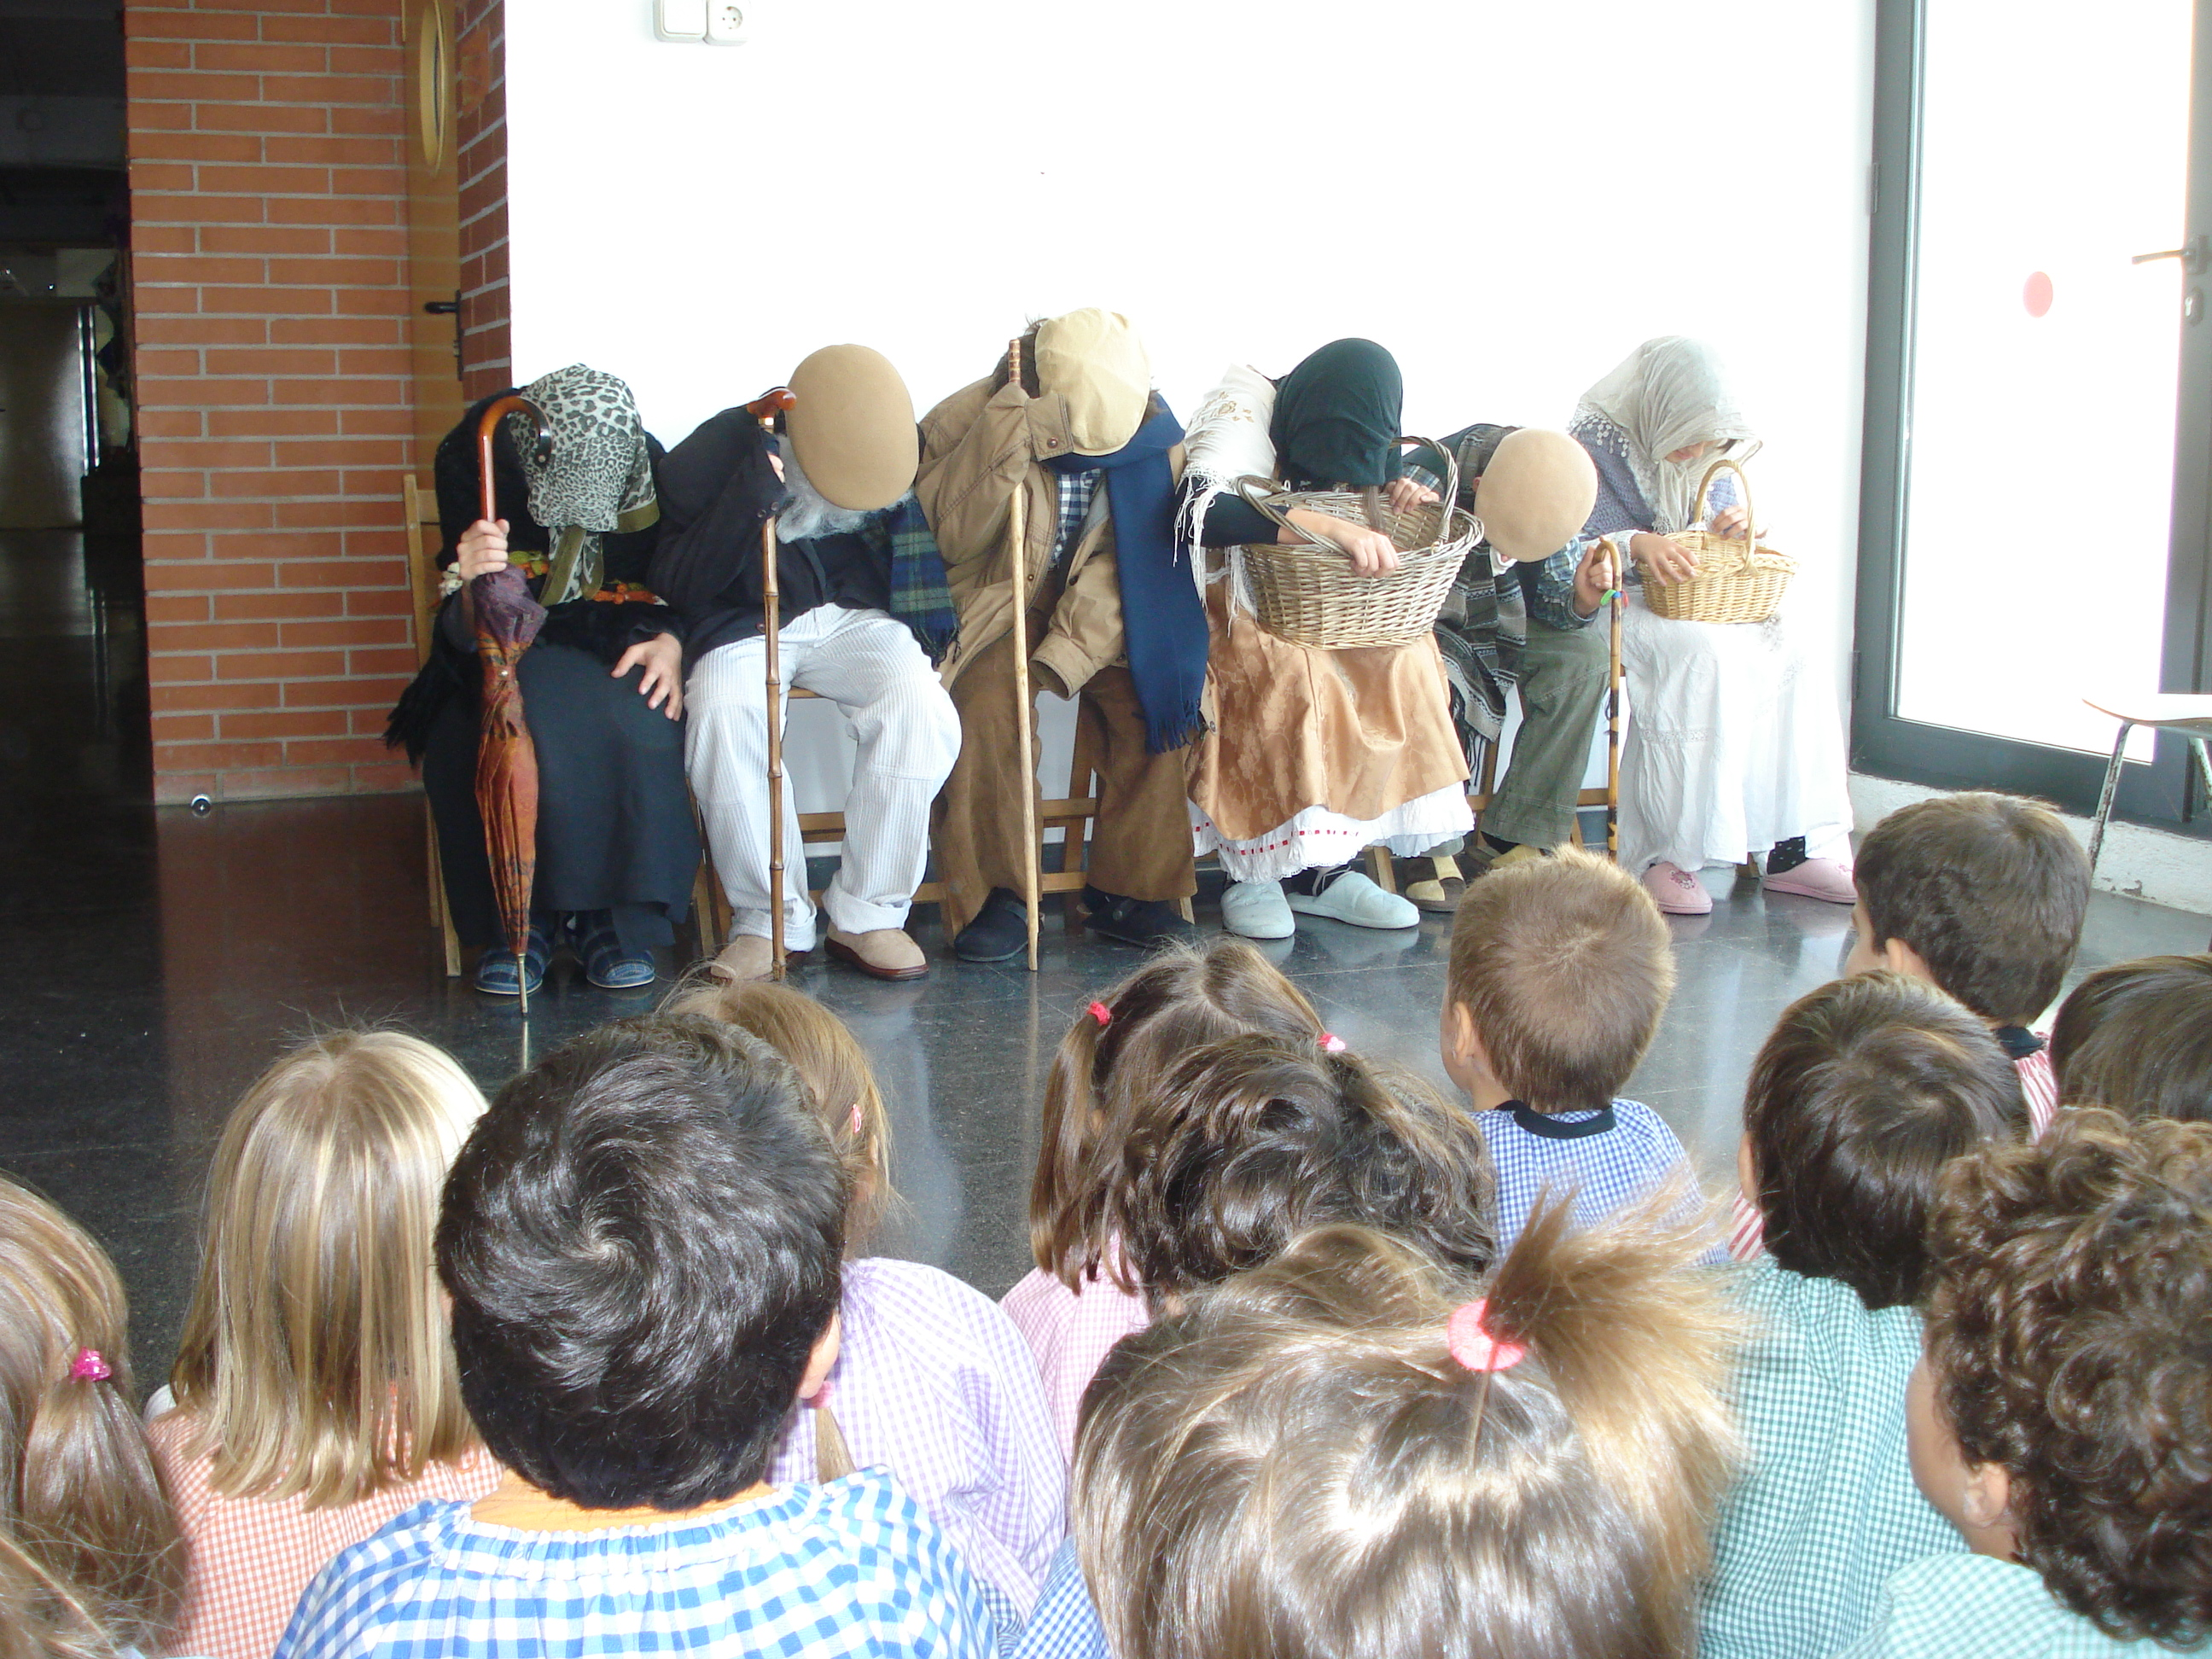
\includegraphics[width=8.5cm,keepaspectratio]{parvulari/img/castanyada_fiotos012.jpg}
El divendres  29 d’octubre,  sis nois i noies de 1r d’ESO,  l’Oriol, la Laia, l’Òscar, el Joel, el Dídac i l’Ariadna,  van anar a fer una representació als nens i nenes de parvulari i primària. Van fer de castanyers i castanyeres. Ho van fer molt bé, tenien moltes ganes de poder-la representar, els feia molta il.lusió.

Els nens i nenes petits es van quedar bocabadats, els va agradar molt, feien una cara de sorpresos, que em sembla que tots s’ho van creure!

El vestuari que portaven estava molt ben trobat; em penso que per a ells no va ser fàcil fer la representació, no només s’havien de disfressar, sinó que també van haver de fer una veu especial, moure els braços i les cames com els vells, i, sobretot, no tenir gens de vergonya! 

A tots els va agradar molt la història que van explicar de la castanya daurada, però també els va agradar moltíssim la cançó que van ballar al final.

Van ser unes castanyeres i castanyers molt valents, simpàtics i gens vergonyosos!!!

\noindent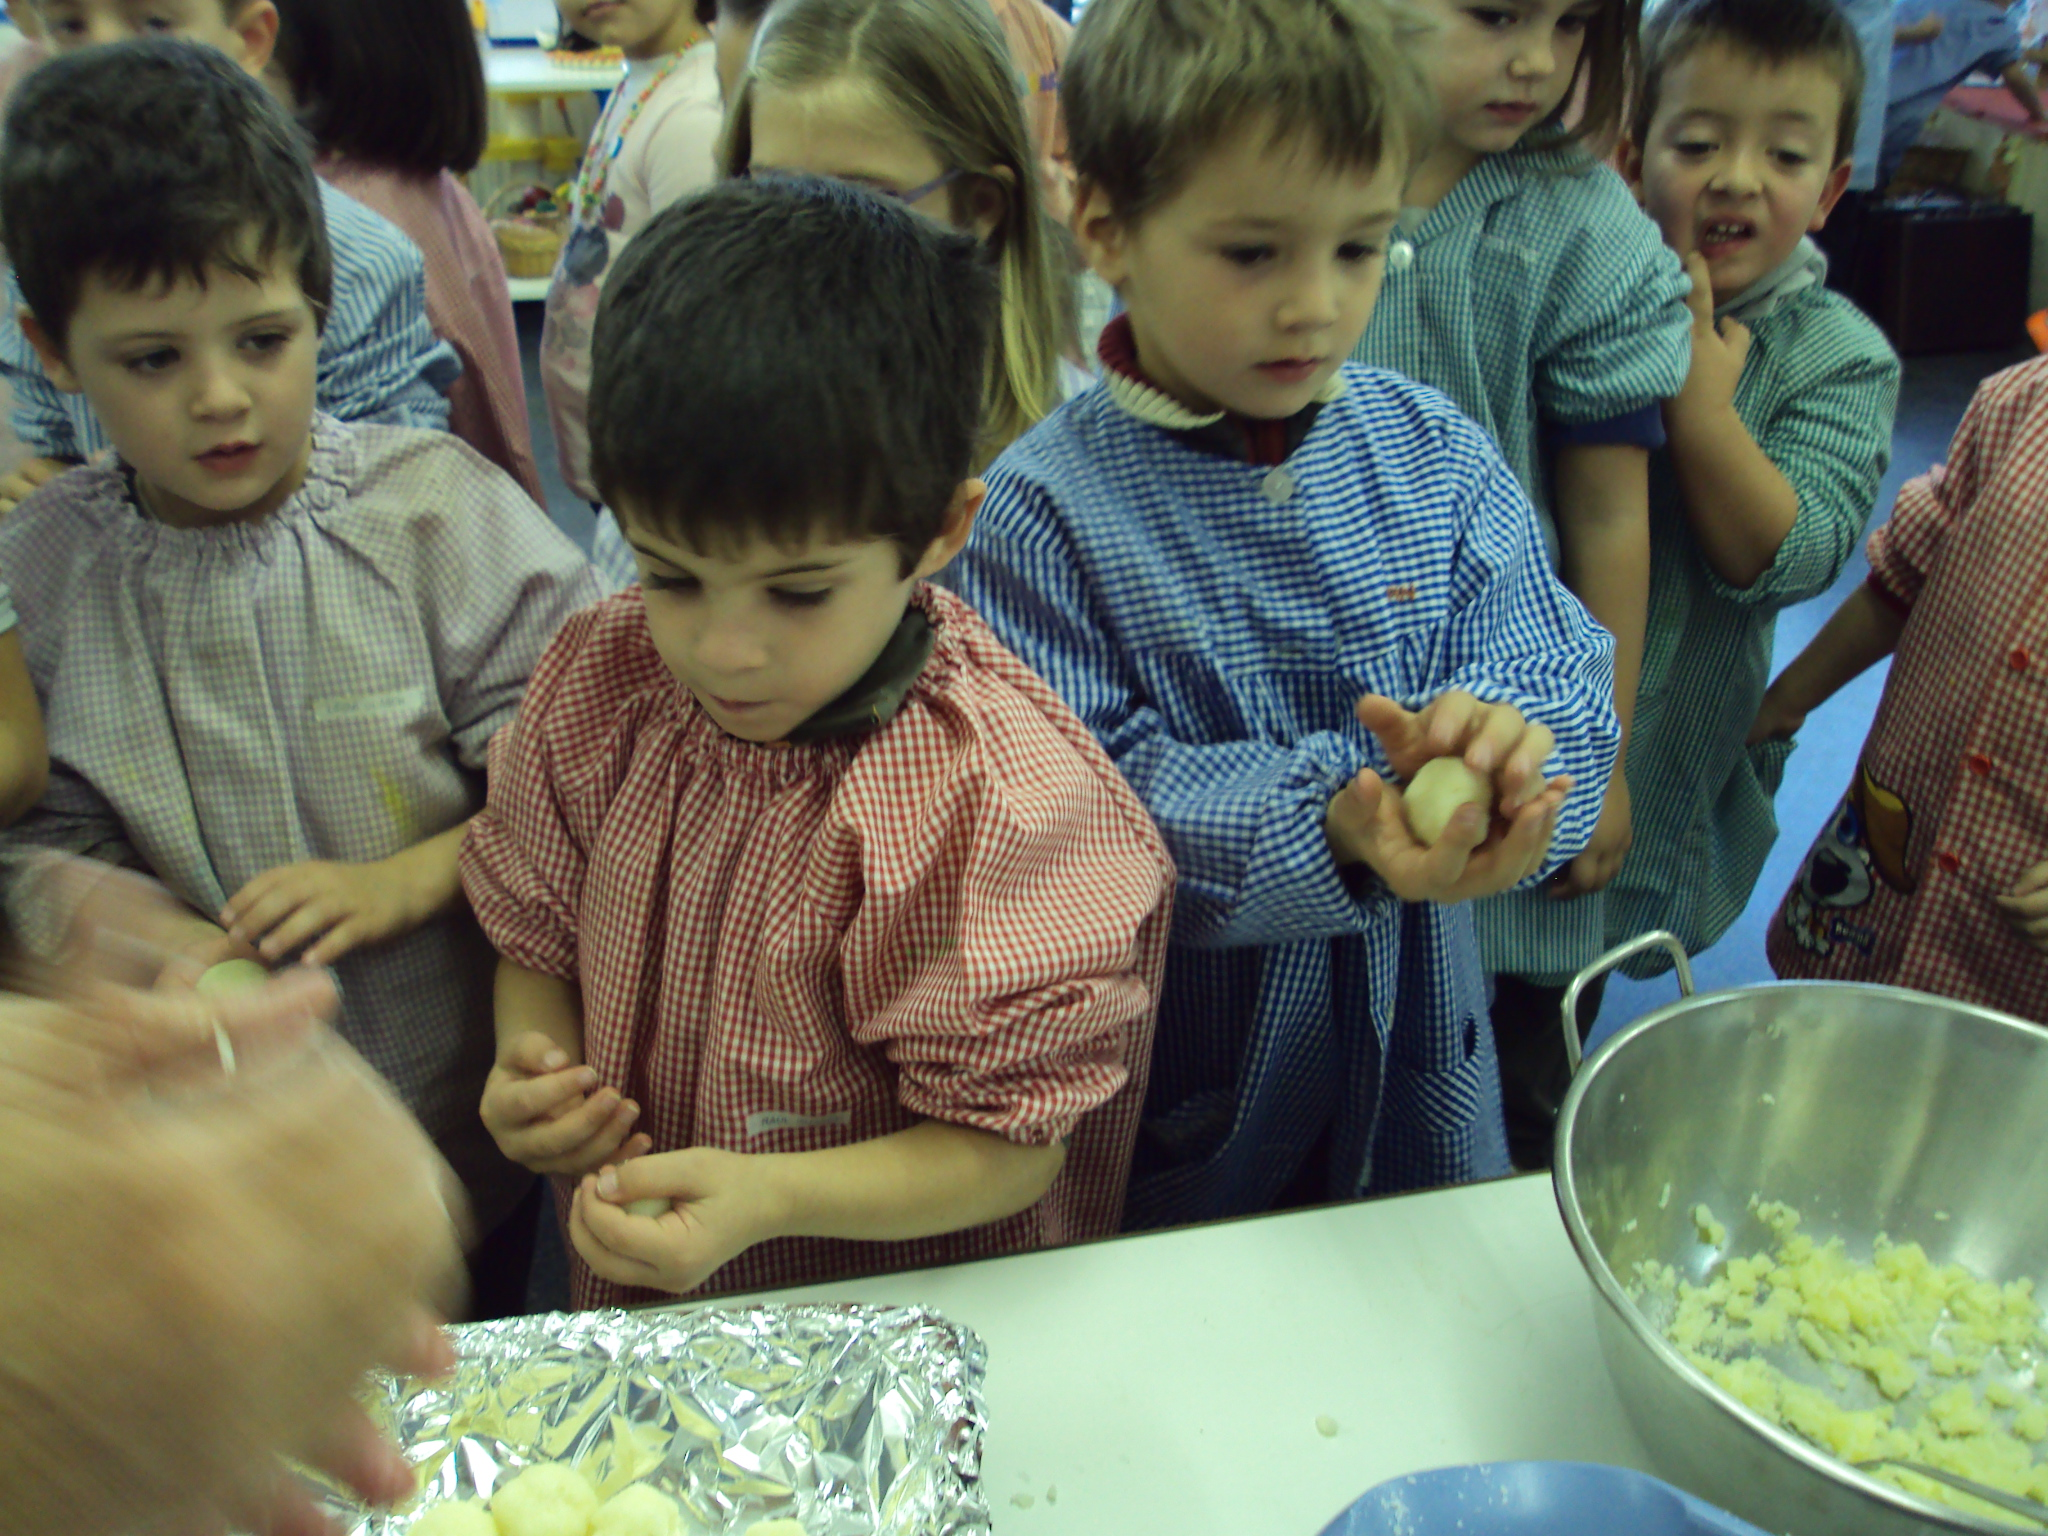
\includegraphics[width=8.5cm,keepaspectratio]{parvulari/img/castanyada_DSC00666.JPG}

\noindent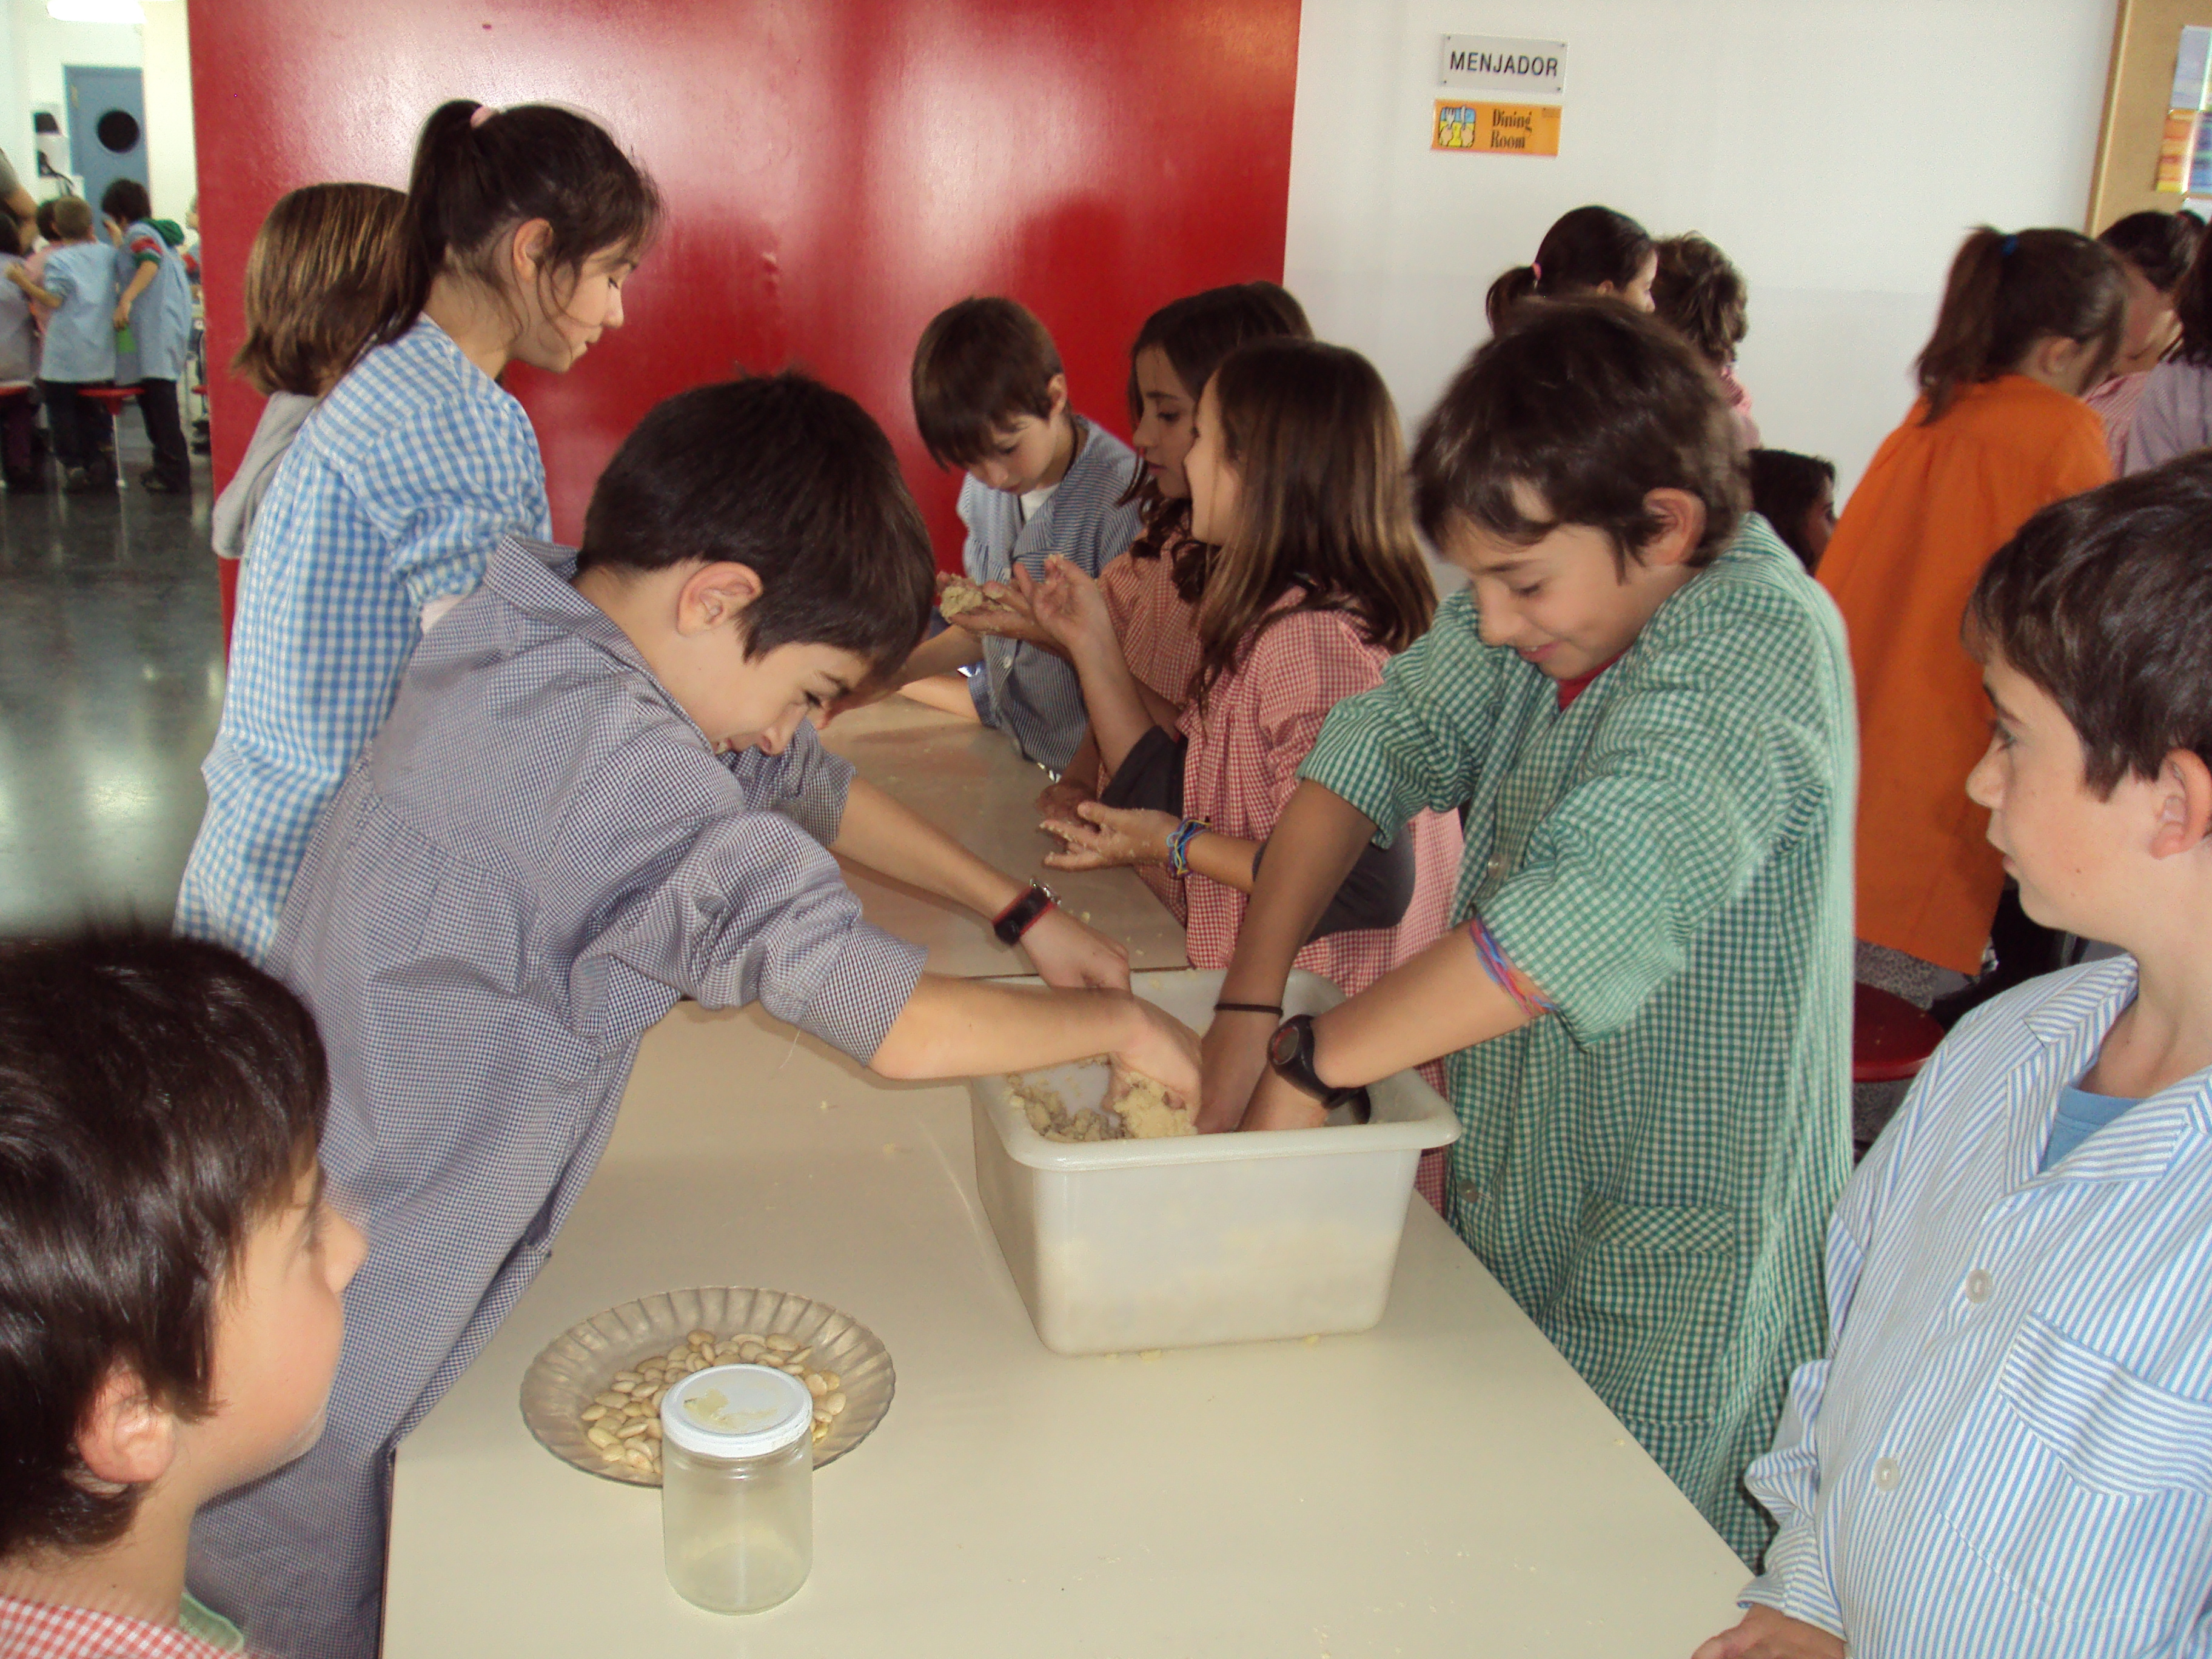
\includegraphics[width=8.5cm,keepaspectratio]{parvulari/img/castanyada_DSC01046.JPG}

\authorandplace{Mariona Medrano}{1r d’ESO}
						
\end{news}


%doc: Revista 3/Res Llibres/ressenyes llibres.docx
\begin{news}
{2} %columnes
{Ressenyes de Llibres}
{}
{Fem Escola}
{03} %pagesof



\subsection*{La Castanyera}

\noindent\fbox{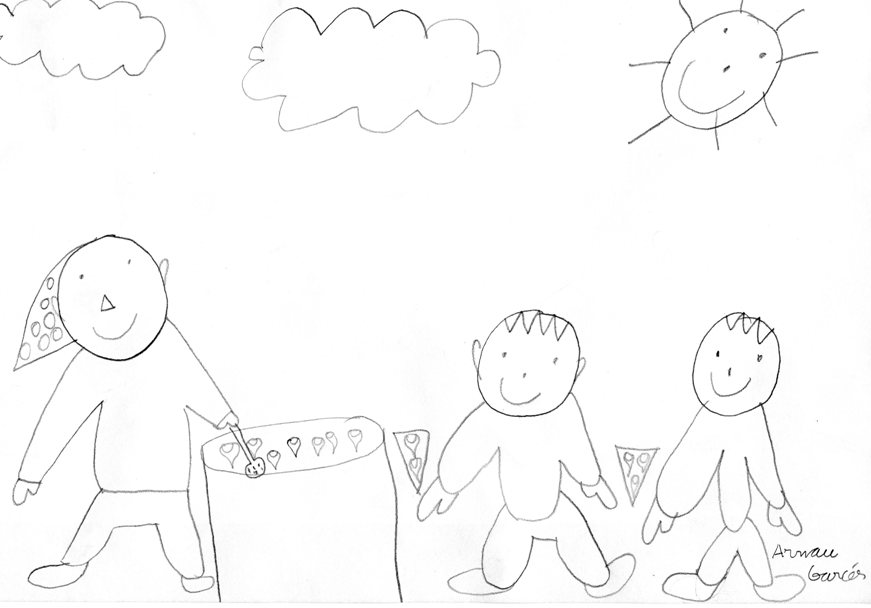
\includegraphics[width=7.5cm,keepaspectratio]{fem_escola/img/ressenya_img002.jpg}}

\emph{Autor: Anna Grau.  Editorial: Combel}

Una castanyera era molt amable, tant, que als nens que no portaven diners els donava castanyes i els deia que portessin els diners un altre dia. Però una altra castanyera, que era dolenta, com que no li compraven castanyes, va pensar robar les castanyes a l’altra. Llavors els nens li van donar castanyes a la castanyera amable, perquè en pogués continuar venent. Al final les dues es van fer amigues i van vendre juntes.

Aquest conte m’ha agradat perquè tracta de l’ amistat.

\authorandplace{Arnau Garcés}{1r de Primària}

\newpage

\subsection*{Els dos núvols amics}
\emph{Autor: Enric Larreula Editorial: Teide }

\noindent\fbox{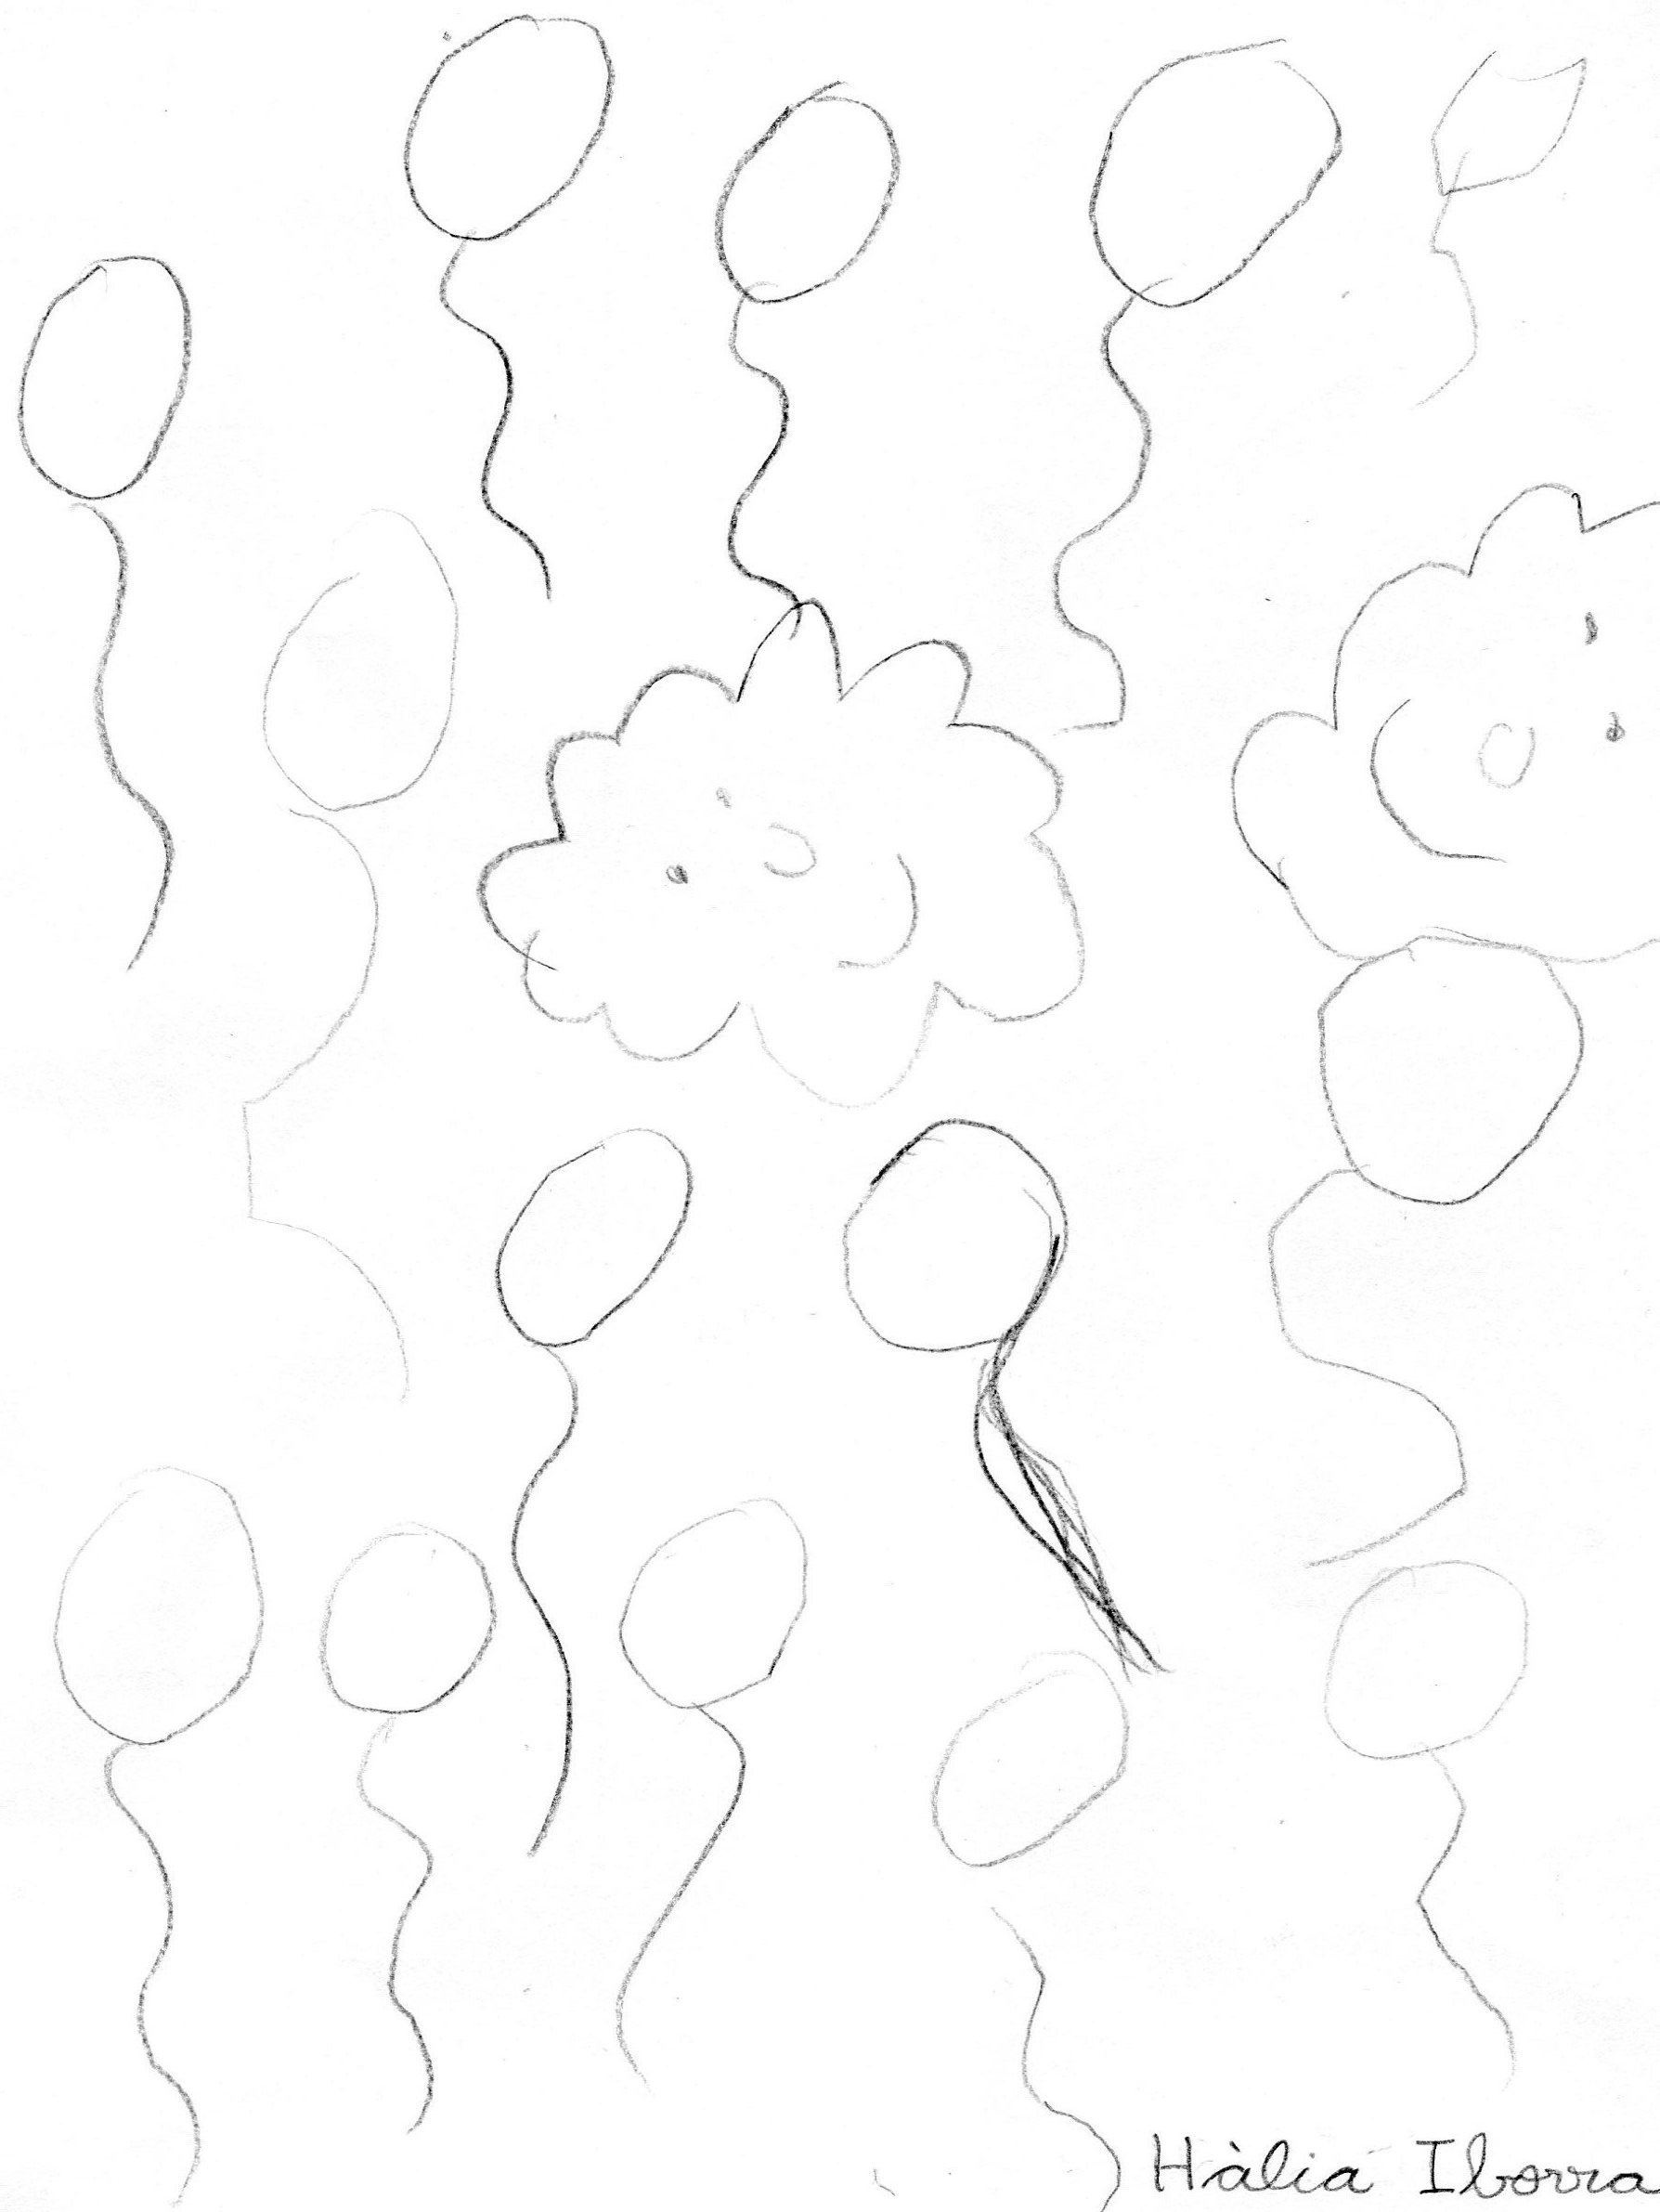
\includegraphics[width=5cm,keepaspectratio]{fem_escola/img/ressenya_img004.jpg}}

Els núvols són molt amics, viatjaven pel temps perquè els agradava estar molt junts. Un núvol estava amb els ocells i els altres estaven solets, els tiraven globus i un dia van caure a terra. Els agradava estar a les muntanyes, a vegades canviaven els colors: un era rosa i l’altre era lila. Un dia va fer molt vent i es van separar una mica, es va posar molt negre el cel i va ploure. Més tard va sortir el sol i els núvols van quedar enterrats.

He triat aquest llibre per l’amistat que demostren entre ells, pels jocs, pels viatges,...

\authorandplace{Hàlia Iborra}{1r de Primària}

\subsection*{La història de l’Ernest}
\emph{Autor: Mercè Company   Editorial: Cruïlla}


\noindent\fbox{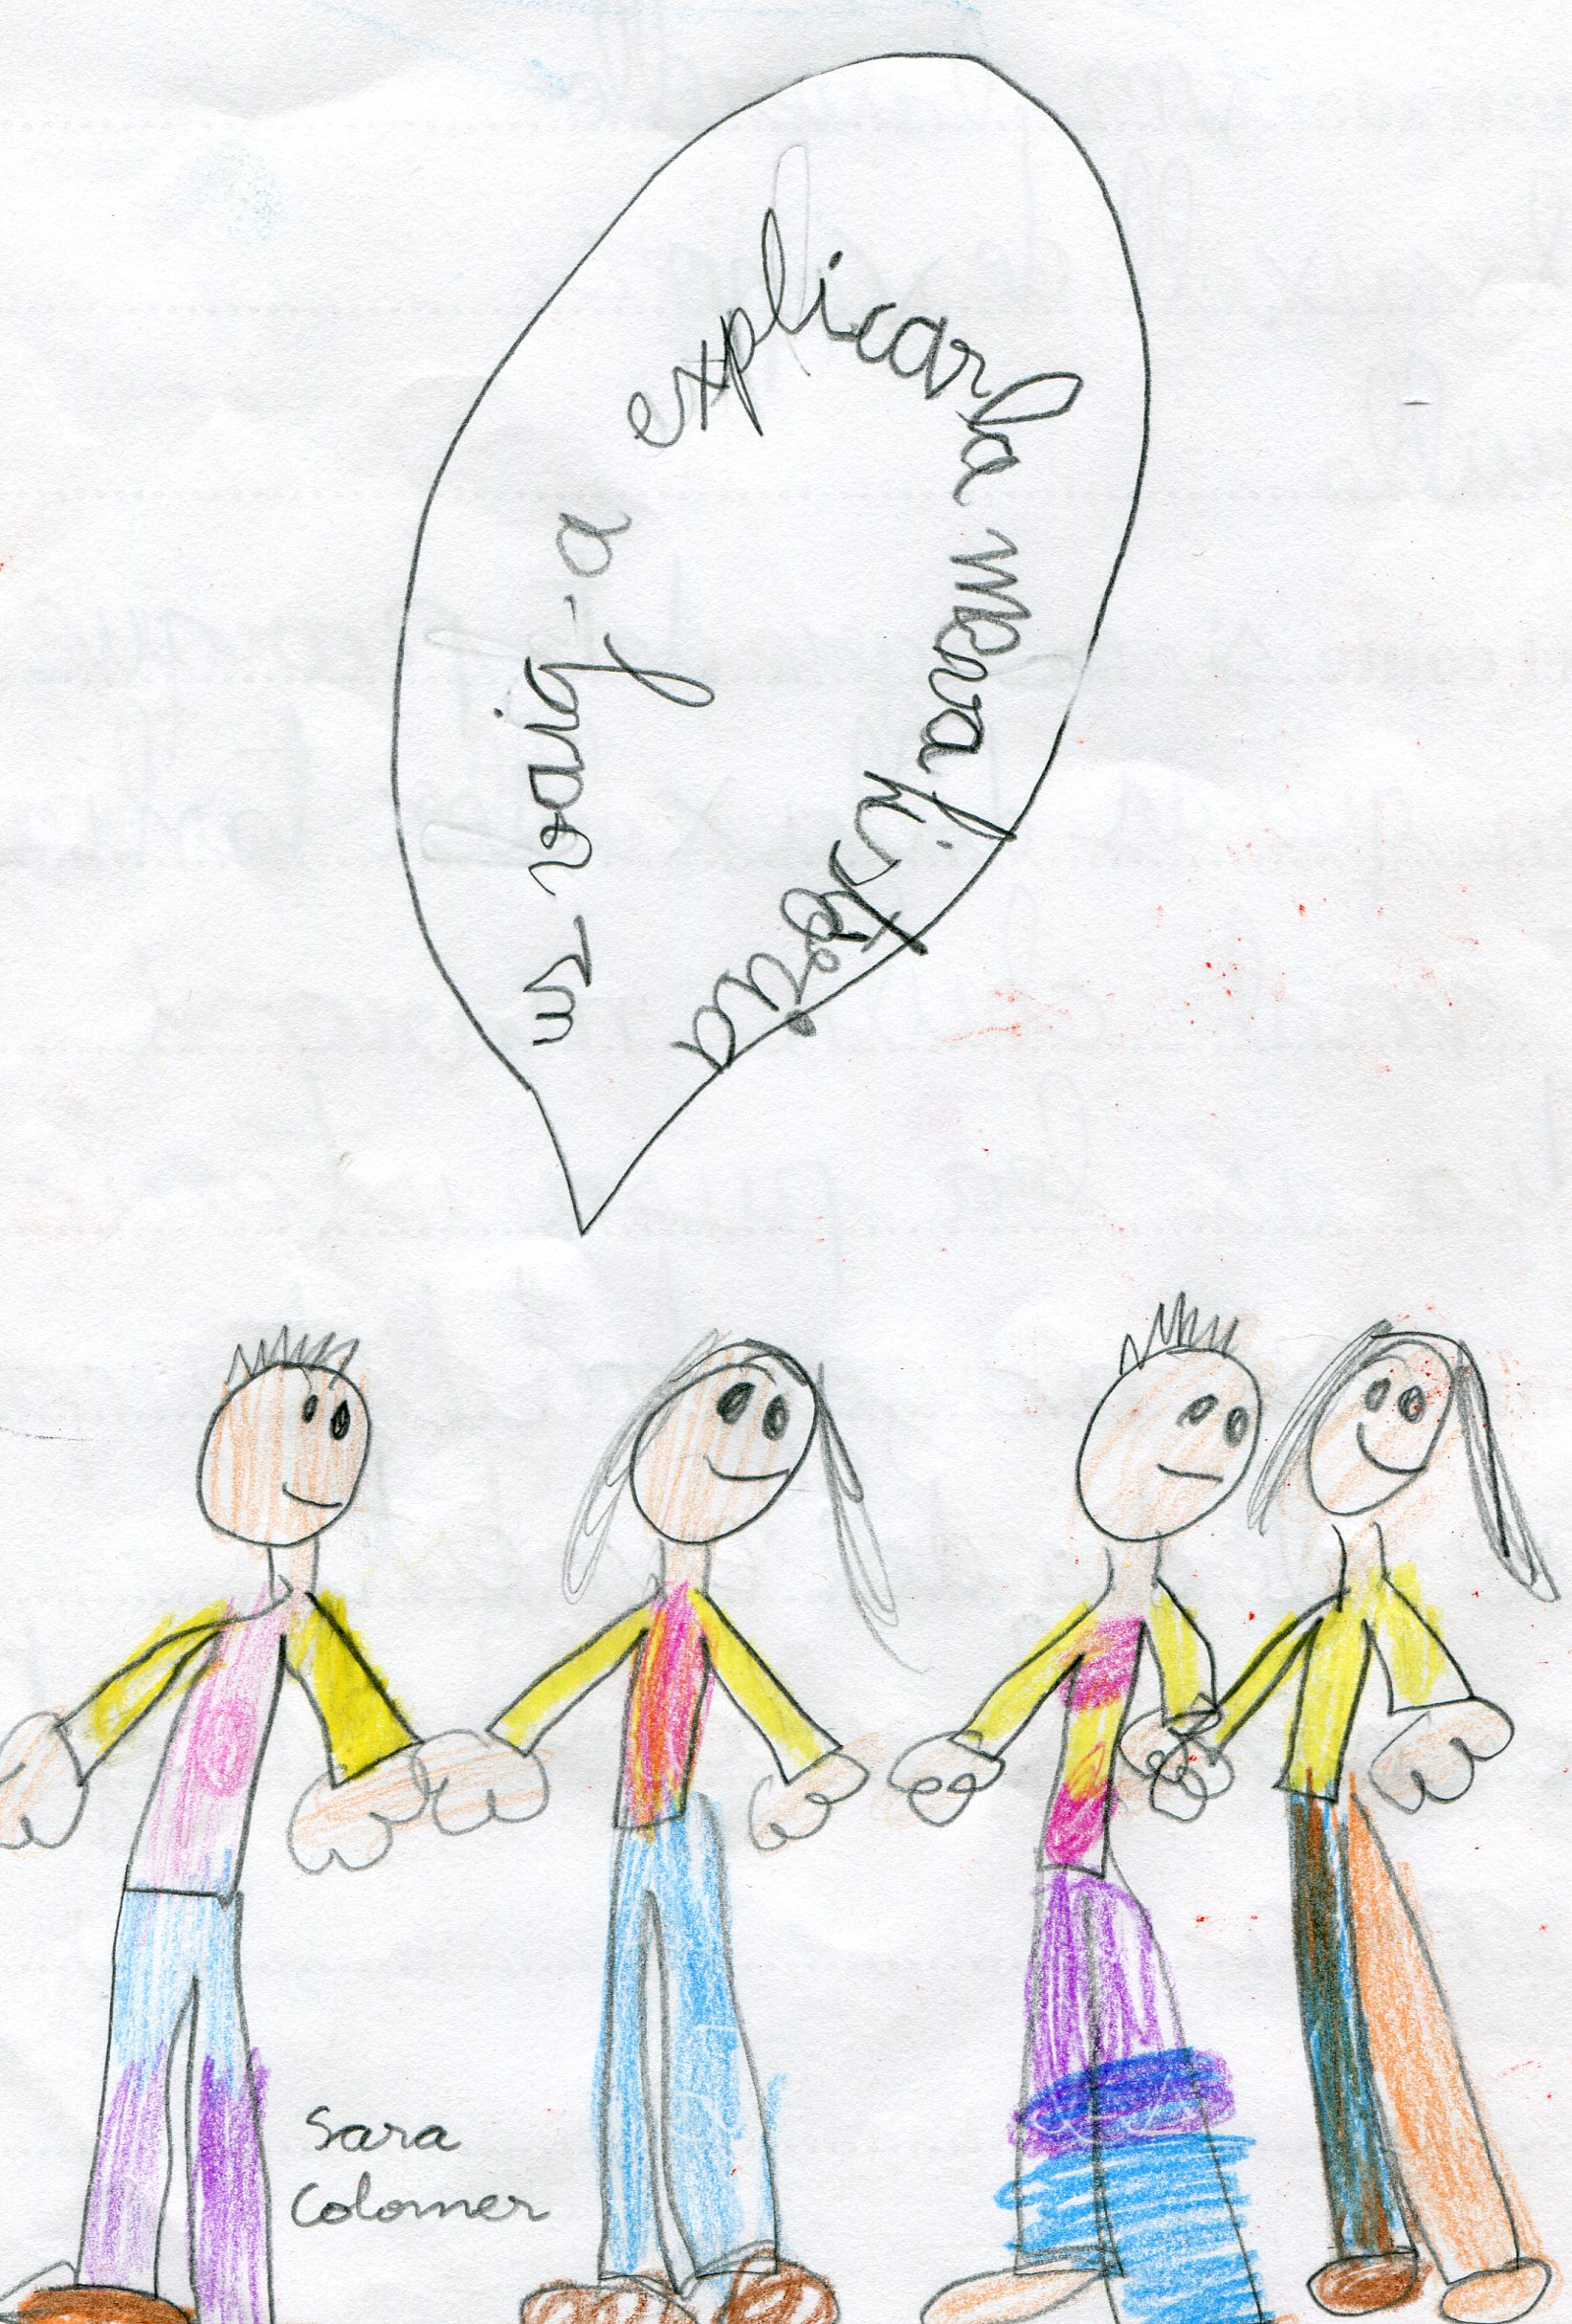
\includegraphics[width=5cm,keepaspectratio]{fem_escola/img/ressenya_img007.jpg}}

Un nen que es diu Xavier tenia un gat marró molt “xulo”, però un dia es va posar histèric.

M’ha agradat aquest conte perquè el dia de l’aniversari de l’Ernest, en Xavier li regala un gat. 

\authorandplace{Sara Colomer}{2n de Primària}


\subsection*{Feu-me cas!}
\emph{Autor: Anke de Vries     Editorial: Cruïlla}

En Kees no estimava el seu germà, en Ron, i la seva mare li va portar un regal que era una pilota i en Kees va estimar el seu germà.

M’ha agradat perquè han fet els dibuixos molt bé.

\authorandplace{Èric Ramos}{ 2n de Primària}

\subsection*{El vell mariner}
\emph{Autor: Geronimo Stilton  Editorial: Destino}

\noindent\fbox{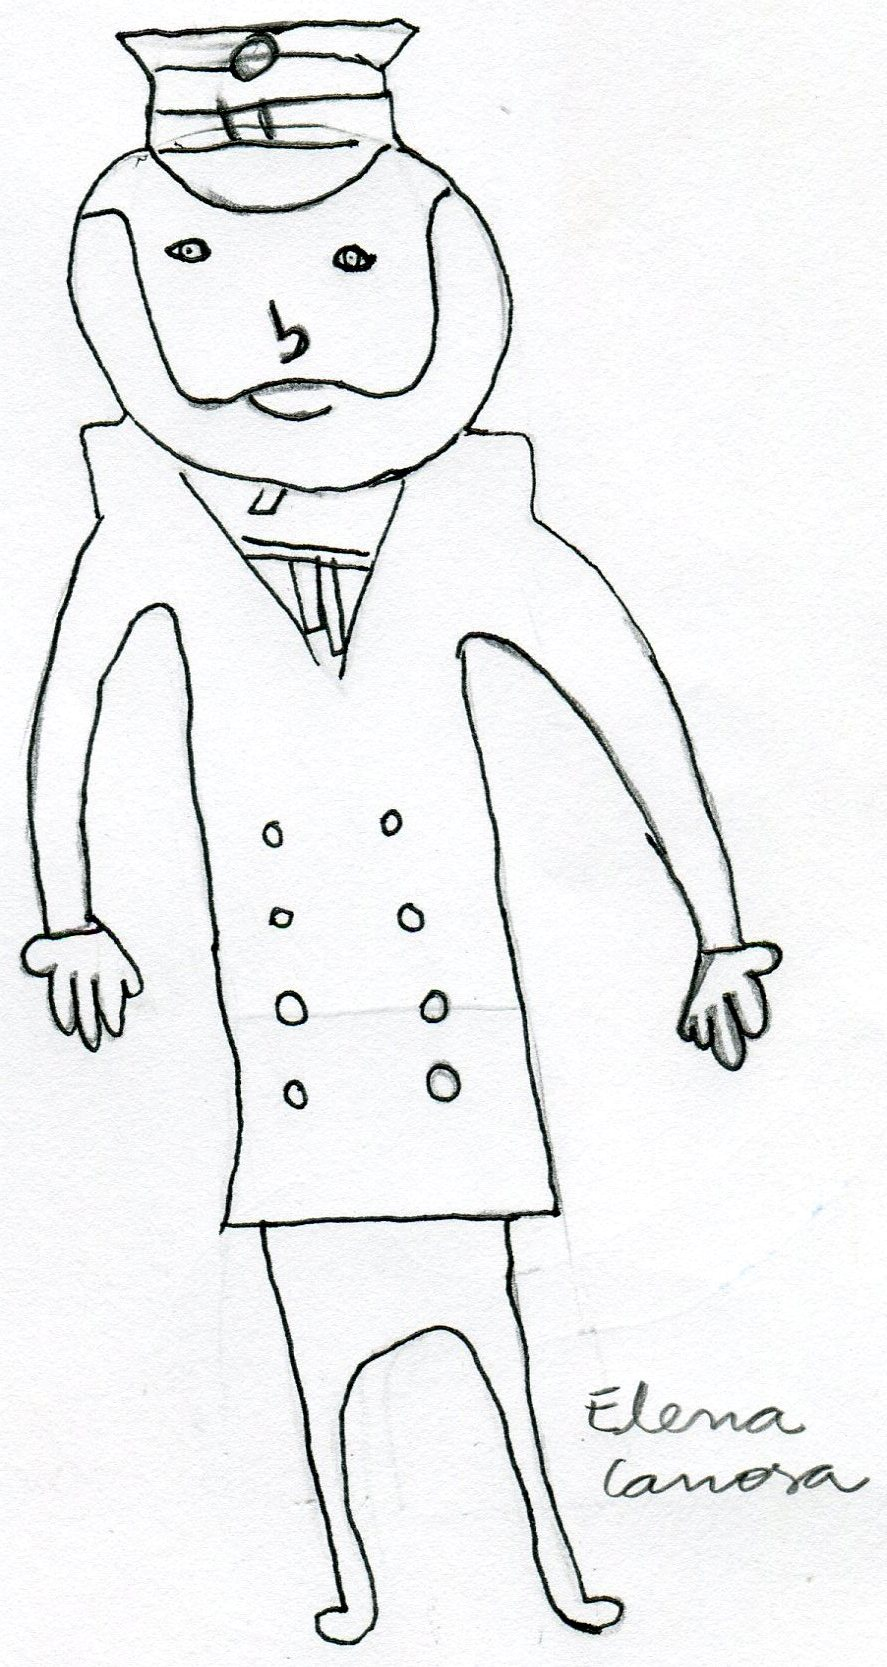
\includegraphics[width=5cm,keepaspectratio]{fem_escola/img/ressenya_img008.jpg}}

Aquest llibre tracta d’un mariner que un dia va a pescar i pesca una sirena.  Se l’emporta a casa seva i li recorda una senyora que anava amb cadira de rodes....

M’ha agradat molt perquè m’agraden els vaixells

\authorandplace{Elena Canosa i Damià Rubio}{3r de Primària}


\subsection*{Llegeix-me si us plau!}
\emph{Autor: Frank Sales.  Editorial: Cruïlla}

\noindent\fbox{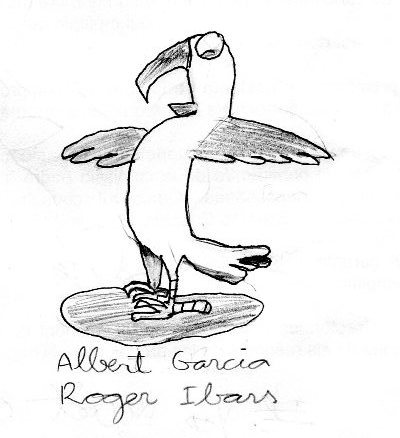
\includegraphics[width=5cm,keepaspectratio]{fem_escola/img/ressenya_img006.jpg}}

Aquesta història parla d’un llibre en un prestatge d’una biblioteca. Aquest llibre té màgia: les lletres parlen! Demanen a la gent que llegeixin perquè no se’ls emportin de la biblioteca. Un dia el llibre cau a sobre de la Laia i comença llegir el conte del lloro Pepet.

M’ha agradat perquè el lloro Pepet comptava d’una manera molt estranya.

\authorandplace{Albert Garcia i Roger Ibars}{ 3r de Primària}


\subsection*{Las aventuras de Ulises}
\emph{Autor: Geronimo Stilton    Editorial: Destino.}

Geronimo Stilton va a una illa, allà troba uns ratolins molt rics i els agrada fer aventures. Entre aquests hi ha el gran capità que no para de parlar d’ Ulisses, que si domina el mar, que si és molt poderós,... Aleshores, Geronimo Stilton va junt amb el capità en un vaixell. De sobte, l’Ulisses neda fins on és el vaixell i amb el seu poder els el trenca. Aquells van en busca de l’Ulisses,... 
	
Aquest llibre m’ha agradat molt per les aventures.

\authorandplace{Axel Santos}{4t de Primària}

\subsection*{Els casos de l’inspector Formiga}
\emph{Autor: Joan de Déu Prats    Editorial: Marge}

\noindent\fbox{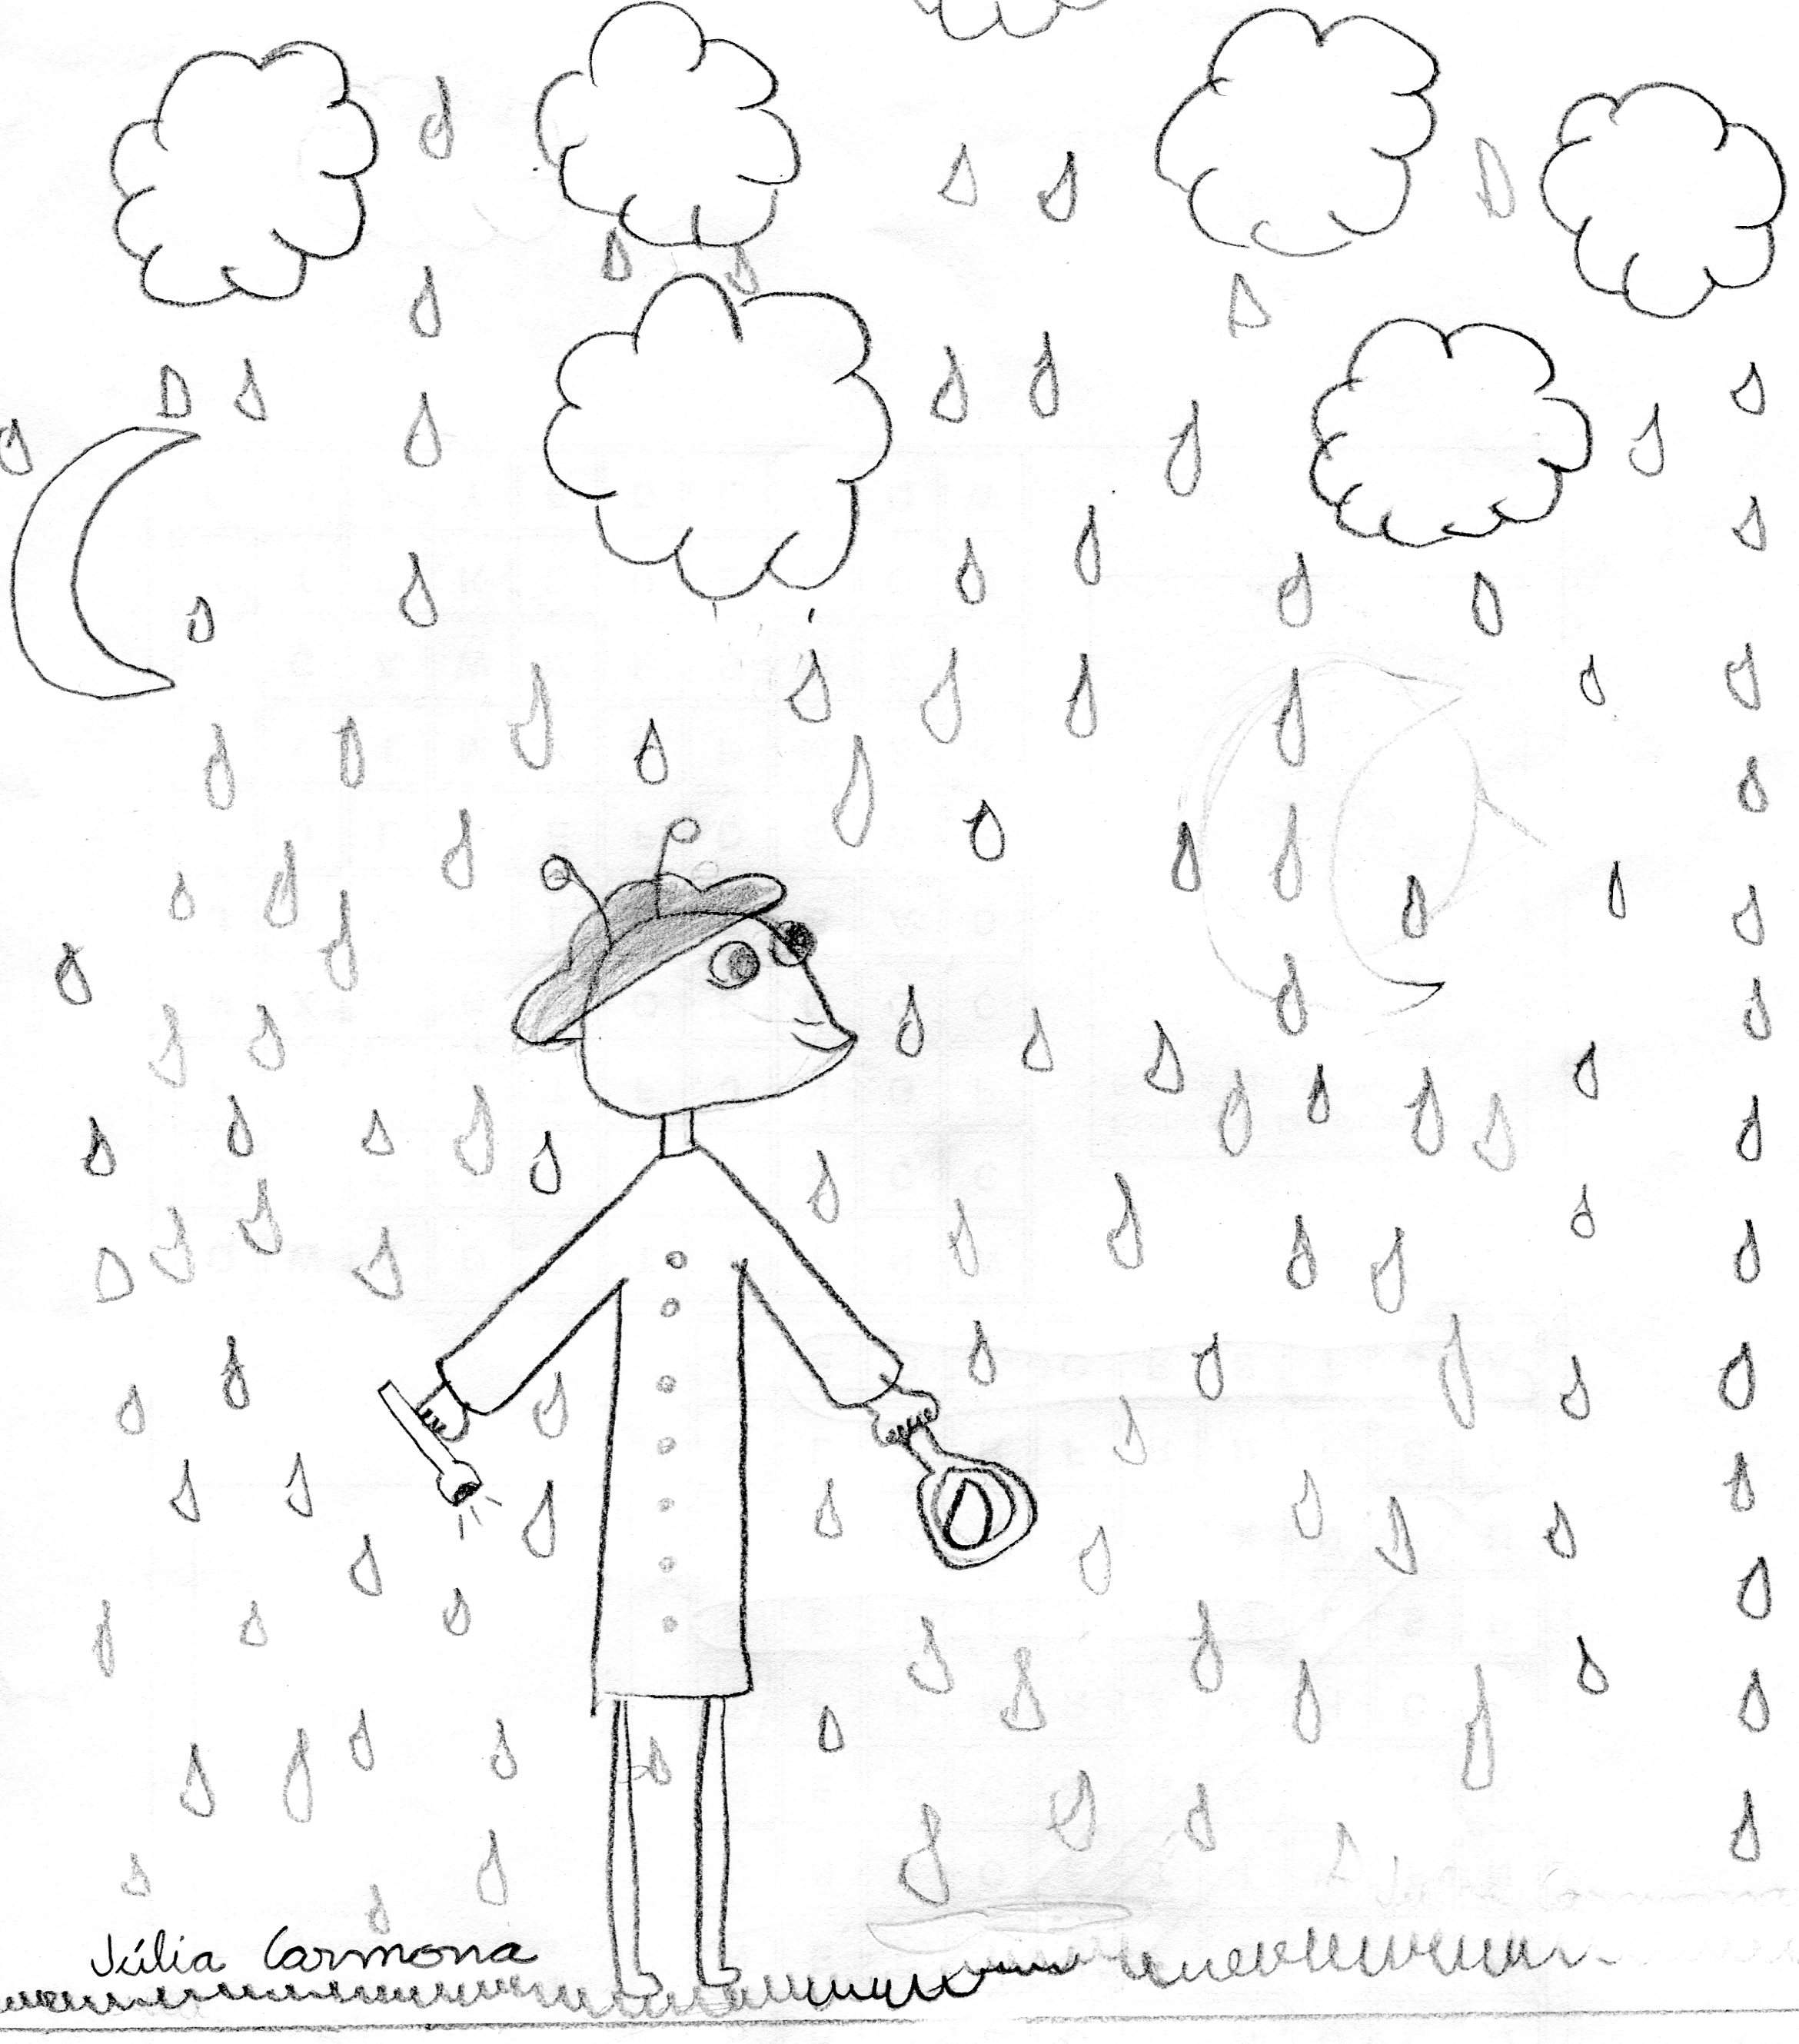
\includegraphics[width=5cm,keepaspectratio]{fem_escola/img/ressenya_img003.jpg}}

És una formiga inspectora que resol casos dels insectes que són assassinats i dels desapareguts. El cas és d’un escarabat que se’l troba mort al carrer i comença a investigar; troba petjades, un ganivet,...

A mi aquest llibre m’ha agradat perquè va d’espionatge i de misteri. El recomano als alumnes de Primària.

\authorandplace{Júlia Carmona}{ 4t de Primària}

\subsection*{Arcanus}
\emph{Autor: Care Santos   Editorial: Planeta}

La història d’aquest llibre ens parla de nens que tenen uns dons especials i que han de cooperar entre ells per salvar el món del malvat Maghul. Aquest llibre forma part d’una col·lecció de dotze títols. A cada un es presenta un dels nens i , a més a més, hi surten bèsties com per exemple un Fènix o un Hipògrif. 

A mi m’ha agradat molt. Us el recomano.

\authorandplace{Oriol Fossas}{ 5è de primària}

\subsection*{Escombres voladores}
\emph{Autor: Ann Jungman    Editorial: Vicens Vives}

Aquest llibre tracta de tres bruixes que a les nits de lluna plena fan encanteris dolents. Dues de les bruixes decideixen no tornar a fer mai més de bruixa. La bruixa que queda s’enfada amb les altres i les insulta. Al cap d’un temps una de les bruixes demana ajuda a les altres. L’ajuden encara que les hagués tractat de mala manera. Finalment la bruixa que no s’havia portat bé es casa gràcies a les seves companyes.

\authorandplace{Carla Salas}{5è de Primària}

\subsection*{T’escriuré}
\emph{Autor: Glòria Llobet.   Editorial: Baula}

L’Anna vivia a Gandia (València). Allà va tenir moltes amistats, especialment  un noi,en Guillem. Un dia els seus pares li comuniquen que se n’han d’anar a viure a Manlleu (Barcelona). Allà haurà de fer noves amistats i superar la seva tristesa.

Aquest llibre m’agrada perquè aquesta noia ha d’anar passant “obstacles” en la seva vida i no saps com reaccionarà. També perquè es una història d’amistat i de comèdia.  

\authorandplace{Marc Luna}{6è de Primària}

\subsection*{Mutació fatal}
\emph{Autor: R.L.Stine  Editorial: Edicions primera plana S.A.}


\noindent\fbox{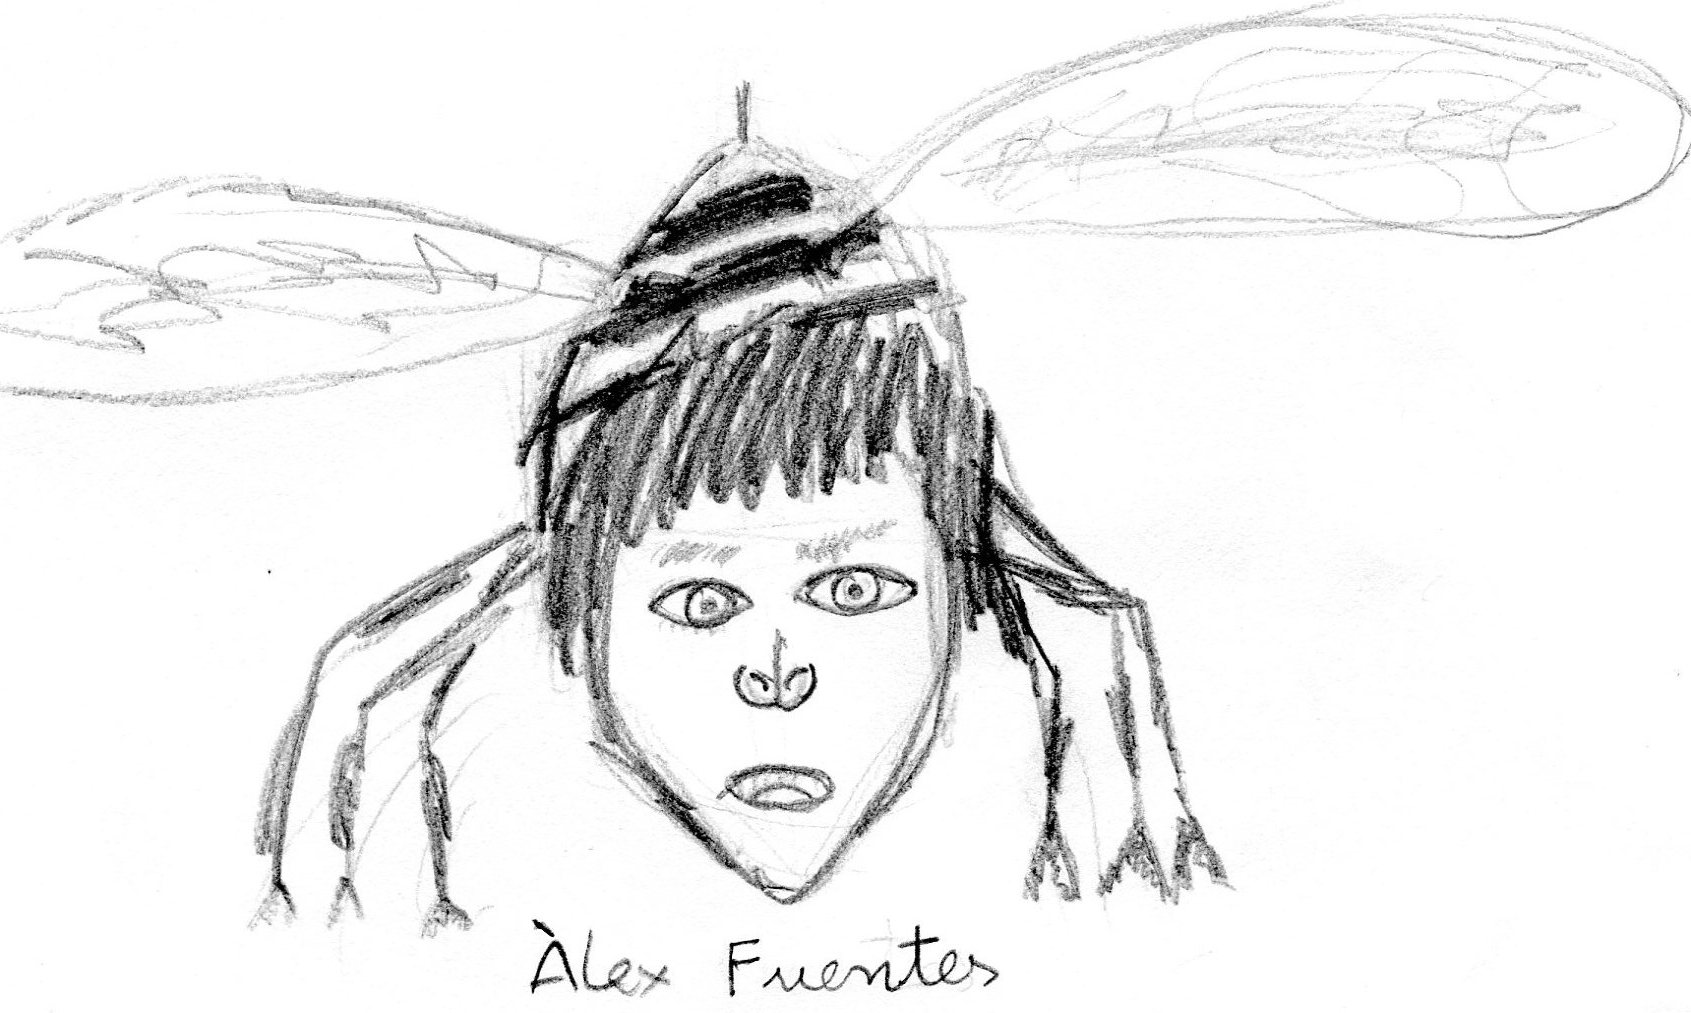
\includegraphics[width=5cm,keepaspectratio]{fem_escola/img/ressenya_img005.jpg}}

Gary Lutz és un nen que no suporta la seva vida, té por de les abelles i se seny empipat per tothom, fins i tot la seva germana es posa amb ell. El senyor Andretti, el seu veí, té un rusc d’abelles. Al nen li fan por les abelles i el senyor Andretti li fa bromes amb les abelles perquè les controla. Un dia ,el nen rep un paper d’una empresa que tenia una màquina que podia canviar les vides en un temps determinat. El nen no s’ho pensa dues vegades i va a l’edifici de l’empresa. A l’edifici, degut a una infiltració d’una abella, Gary Lutz es convertirà en l’insecte que menys li agrada.


\authorandplace{Àlex Fuentes}{6è de Primària}



\subsection*{Lior}
\emph{Autor; Pradas, Núria. Ed.}
 
Us recomano aquest llibre perquè és molt entretingut. Parla d’un món del futur on no hi ha sentiments ni llibertat, només val l’esport i la competició. En Lior descobrirà que hi ha altres habitants d’aquesta societat que pensen de forma diferent i lluitarà per aconseguir un món diferent.

\authorandplace{Joan Colldecarrera}{1r ESO}


\subsection*{Cartas de invierno}

\emph{Autor; 	Fernández Paz, Agustín. Ed.SM}

El pintor Adrián Novoa, aconsejado por su amigo Xavier, compra una casa en una aldea de Galicia. Es la casa de sus sueños. En ella quiere encontrar la paz necessaria para encontrar nueva inspiración en su pintura. Pero la casa esconde un profundo y oscuro misterio que atrapa a Novoa como un imán.

Recomiendo este libro porque te engancha desde el principio, es decir, no puedes parar de leer, porque cada vez que acabas un capítulo quieres leer el siguiente. És un libro de misterio y algo de terror.

\authorandplace{Sergi Cervera}{1r d’ESO}



\subsection*{Fi de curs a Bucarest}
\emph{Autor; Pinyol, Joan. Ed. Baula}

Radu Petrescu és un noi que ha de marxar de casa perquè el seu pare l’ha obligat a robar i el persegueix la policia.

Radu se’n va de Cosbuc, el seu poble, cap a Bucarest, la capital de Romania.

Durant el viatge cap a Bucarest coneix  uns nois ( Vasile, Moisei ,l'Ovidi i en Juliu) que pertanyen a una organització que no vol permetre que Romania entri a La Unió Europea. En Radu s’uneix a ells ja que no té diners.

Un grup  d‘estudiants catalans arriba a Bucarest de viatge de fi de curs de 4t   d’ESO, entre ells un noi anomenat Raül. 

El dia de l’arribada dels catalans el grup d’en Radu i d’en Raül es troben en  un parc  i es barallen. Durant aquest enfrontament els amics d’en Radu li roben la càmera a en Raül.

En Raül havia de recuperar la càmera fos com fos, ja que era del seu pare.  

En Radu li promet que  l’ajudarà a recuperar la càmera. Uns dies més tard en Radu desapareix.

En Raül i la Tatiana, una amiga romanesa, presenten una denúncia per la desaparició d’en Radu Petrescu. ...

 I la història continua..............

\authorandplace{Carla Jiménez}{2n ESO}

\subsection*{Sis històries al voltant d’en Màrius}
\emph{Autor: Sierra i Fabra, Jordi. Ed Planeta	}

Aquest llibre tracta de la vida d’un noi, en Màrius, que relata la seva vida des que neix fins als divuit anys; no obstant, ell no n’és el narrador sinó les diferents persones que ens l’expliquen, gent del seu entorn, família i amics.

Cada història és un any o dos de la seva vida, i cada persona explica el que va viure amb en Màrius

Si el llegiu veureu que en Màrius acaba tenint problemes amb les drogues i que no li serà gens fàcil sortir-se’n.

Aquest llibre l’he trobat entranyable i fascinant, és d’aquells que el llegiries més d’una vegada

\authorandplace{Maria Garcia}{ 3r ESO}



\subsection*{Pots comptar els estels?}
\emph{Autor: Lowry, Lois. Ed La Magrana}

Som a l’any 1943 i, per a l’Annemarie , viure a Copenhaguen és una barreja de rutina, d’escassetat de menjar i d’opressió per la presència constant de les tropes nazis.
La seva família ajuda els seus veïns a escapar de Dinamarca quan els nazis comencen a endur-se els jueus, i amaguen l’Ellen, la millor amiga de l’Annemarie, tot i córrer el risc de ser descoberts.

\authorandplace{Davínia W. Vilagrasa}{ 3r d’ESO}

\subsection*{Bitllet d’anada i tornada}

\emph{Autor: Lienas, Gemma. Ed. Estrella Polar}

Bitllet d’anada i tornada és el testimoni d’una noia que pateix anorèxia i és ingressada a l’hospital on coneix a altres noies que tenen el mateix problema. Però la Marta, la protagonista, no vol engreixar-se de cap de les maneres ja que té por de patir bulímia. Allà recorda com era la seva vida, abans d’ingressar a l’hospital, amb la família, amb el Rcky, la seva parella, i amb la seva millor amiga, la Clàudia.
Aquesta novel.la la trobo molt recomanable ja que és una història sobre la realitat de molts joves d’avui en dia, és un llibre que et mentalitza. Crec que l’autora sap com explicar i parlar d’aquest tema tan delicat, ens fa veure que l’anorèxia no és cap broma ni cap diversió. És una malaltia molt greu. 

\authorandplace{Raquel Madrenas}{4t ESO}


\subsection*{Memòries d’Idhum}

\emph{Autora: Gallego, Laura. Ed. Cruïlla}

És un llibre que combina molt bé la història d’amor amb la fantasia i un conjunt d’éssers fantàstics
La trama es du a terme a la terra i a Idhum, un món màgic on un tirà anomenat Ashran és al poder. En Jack, la Victòria i els seus amics, els anomenats “la resistència”,  lluitaran per aconseguir la llibertat de la seva terra i la seva i també pròpia.. Escenaris com boscos que creixen a grans velocitats, deserts mortífers, muntanyes canviants i paisatges gelats on hi viuen gegants..., tot plegat és una explosió de fantasia i màgia
\authorandplace{Esteve Pérez}{4t ESO}

\end{news}


\newpage
%doc: Revista 3/PresentacioRB/presentacio.docx
\begin{news}
{2} %columnes
{Presentació del llibre: El documental com a estratègia educativa}
%index: El documental com a estratègia educativa
{El Ramon Breu, professor  de l’escola i company nostre, el dia 20 d’octubre va presentar el seu darrer llibre : EL DOCUMENTAL COMO ESTRATEGIA EDUCATIVA, a la Biblioteca plaça d'Europa}
{Fem Escola}
{250} %pagesof

\noindent
\includegraphics[width=9cm,keepaspectratio]{fem_escola/img/llibre_PA200015b.jpg}

%Amadeu Torner, 57 de l’Hospitalet de Llobregat.

Participaren de la presentació  David Urrea, director de la Biblioteca Plaça d'Europa, Cinta Vidal, directora d'Edicions de l'Editorial Graó i Alba Ambròs, professora de la Facultat d'Educació de la Universitat de Barcelona.

Va ser un acte entranyable i íntim;  en Ramon va estar molt ben acompanyat per la família, els companys, els  amics i per professionals diversos. 
A més, la biblioteca és un lloc molt significatiu i proper per en Ramon ja que està ubicada en  l’entorn on ell ha passat la infància i bona part de la seva vida.

Com a professionals de l’ensenyament valorem aquest llibre com una bona eina didàctica per a l’educació en valors i per a l’estudi i anàlisi del documental a les aules. Estem molt orgullosos de la il·lusió, dedicació i esperit de renovació que el nostre company és capaç d’aportar a l’ensenyament tot elaborant diferents materials didàctics i de reflexió que permeten millorar la qualitat pedagògica de les escoles. 

\authorandplace{Per molts anys, Ramón !}{}

\end{news}


%doc: Revista 3/Banc dels aliments - Arnau Bilbao (3r d'ESO).docx

\begin{news}
{2} %columnes
{Xerrada sobre el Banc dels Aliments}
{El divendres 12 de novembre,  un dels 92 voluntaris del banc dels aliments va venir a l’escola Solc per fer-nos una xerrada als nois i noies de 3r d’ESO sobre el Banc dels Aliments}
{ESO}
{404} %pagesof


Va ser una xerrada molt instructiva i alhora molt divertida ja que el senyor que va venir ens va fer la xerrada d’una manera diferent a altres xerrades que havia escoltat jo anteriorment. Ens va explicar moltes coses: què era el banc dels aliments, de què s’encarregava, què o qui el formaven...

Segons ens va explicar el voluntari, el banc dels aliments és una entitat que s’encarrega de recollir aliments per tota Catalunya, en instituts i escoles que col·laboren en la recollida d’aliments que es produeix un cop cada any durant una setmana. També recullen excedents de marques de menjar (Tarradellas, Ferrero Rocher, etc...). Tot aquest menjar s’aconsegueix gratis. Un cop tenen el menjar el guarden uns dies fins que gent pobra d’aquí, a Catalunya, en necessita per alimentar-se,  ja que no tenen prou diners per aconseguir-ne. El menjar es reparteix amb 4 furgonetes que tenen entre tots els voluntaris. A vegades al Banc dels Aliments els falta algun tipus determinat de menjar, llavors fan una mena de subhasta per comprovar quina marca d’aquell aliment els el donen més barat i llavors el compren. En el Banc dels Aliments no s’accepten ni begudes amb alcohol ni queviures quasi caducats;  tot i així aquests aliments sí que els accepten perquè no els hagin de portar a l’abocador.

Tot això ens  ho va explicar, també,  amb un “powerpoint”. En el “powerpoint” s’hi explicava què era el banc dels aliments (bé, ens explicava el mateix que el voluntari). Ens vam divertir molt en aquesta xerrada perquè el voluntari era molt divertit i quan algú feia alguna pregunta interessant li donava un caramel! A part d’això també va ser una xerrada molt instructiva.

Ens ho vam passar d’allò més bé fent feina normal i corrent.

També ens va dir que, si volíem, podíem anar al Banc dels Aliments a col·laborar. Un company de la nostra classe ho va fer fa pocs dies, i tant ell com jo us animem a presentar-vos, si voleu, com a voluntaris del Banc dels Aliments, una cosa que s’agrairia molt ja que allà tenen molta feina per fer i poca gent per fer-la. Podeu trobar més informació a www.bancdelsaliments.org.

\authorandplace{Arnau Bilbao}{3r d’ESO}

\end{news}



\newsection{Parvulari}

%doc: Parvulari/que_es_el_primer.doc
\begin{news}
{2} %columnes
{Què és el primer que treballem quan arribem a l’escola ?}
{\noindent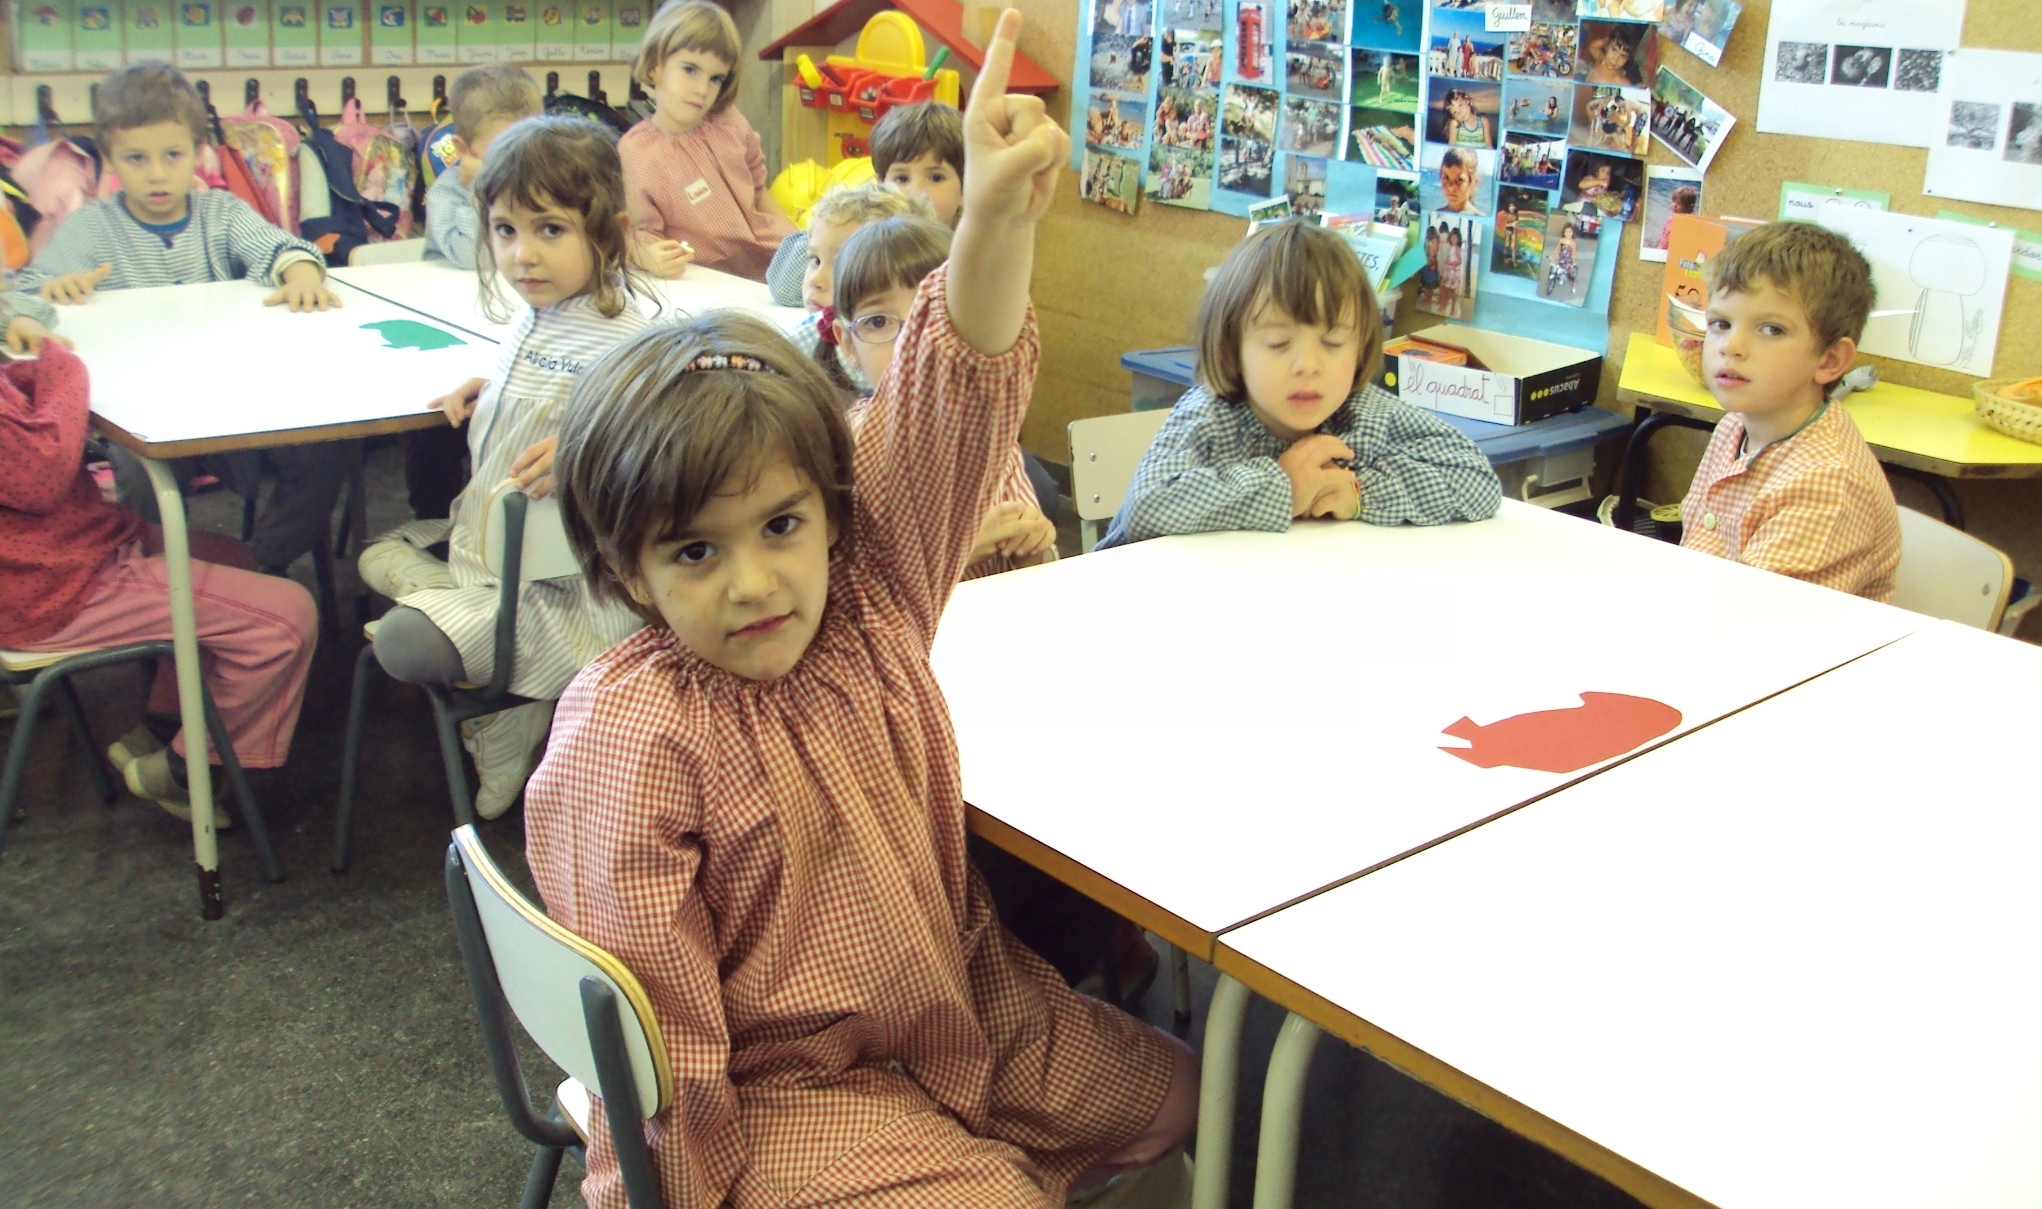
\includegraphics[width=18cm,keepaspectratio]{parvulari/img/foto3b.jpg}}
{Parvulari}
{21} %pagesof

Entenem com a hàbits aquelles situacions que es repeteixen de forma sistemàtica i ens ajuden a agafar seguretat i a poder preveure els fets.

També ens ajuden a estructurar-nos, a orientar-nos i a evolucionar millor.
Els bons hàbits també possibiliten una relació de convivència positiva amb tots i amb tot.

Quan més estructurats estiguem, més preparats estarem per la nostra autonomia personal. 

Els hàbits s’han de treballar a casa i a l’escola. A mida que anem assolint els diferents hàbits ens sentirem més segurs, tranquils i amb ganes d’aprendre.
Aprendre a observar els petits progressos que fa cadascú, dia a dia,  i saber valorar-los és per a la persona  una motivació important i necessària per continuar avançant.

Aquests  són alguns dels hàbits que aprenem a la classe de cargols, a la classe de pingüins i a la dels elefants.

Els cargols expliquen: hàbits d’autonomia
La Metis ens ensenya a rentar-nos les mans, abans ho fèiem  malament i no ens quedaven netes , ara ja ho fem bé perquè som grans .


\noindent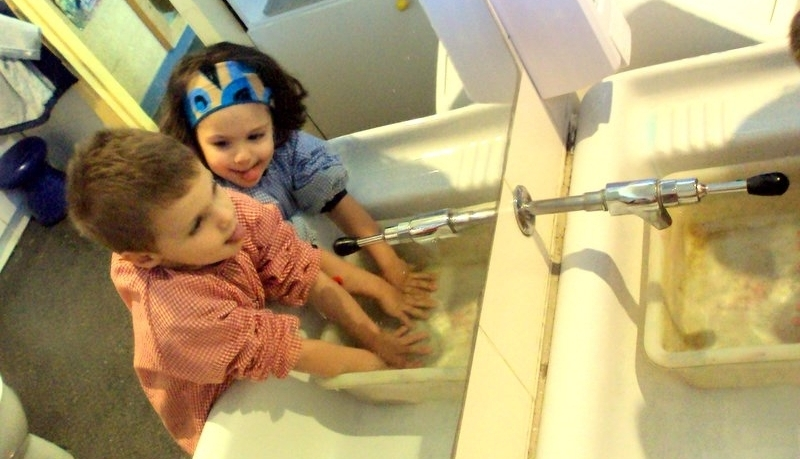
\includegraphics[width=9cm,keepaspectratio]{parvulari/img/foto1b.jpg}

També hem après a treure’ns la jaqueta i posar-nos la bata nosaltres solets i, quan no podem, ens ajuda la Metis i el Martí


\noindent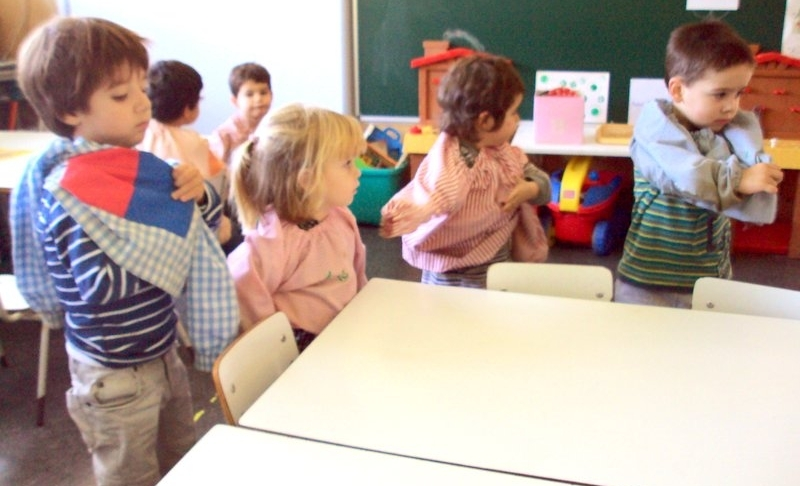
\includegraphics[width=9cm,keepaspectratio]{parvulari/img/foto2b.jpg}



Els pingüins expliquen: hàbits socials

A la classe dels pingüins,  la Rosa ens ensenya que quan volem dir una cosa  hem d’aixecar la mà i,  si hi ha moltes mans alçades, ens hem de saber esperar i no parlar tots alhora.



%\noindent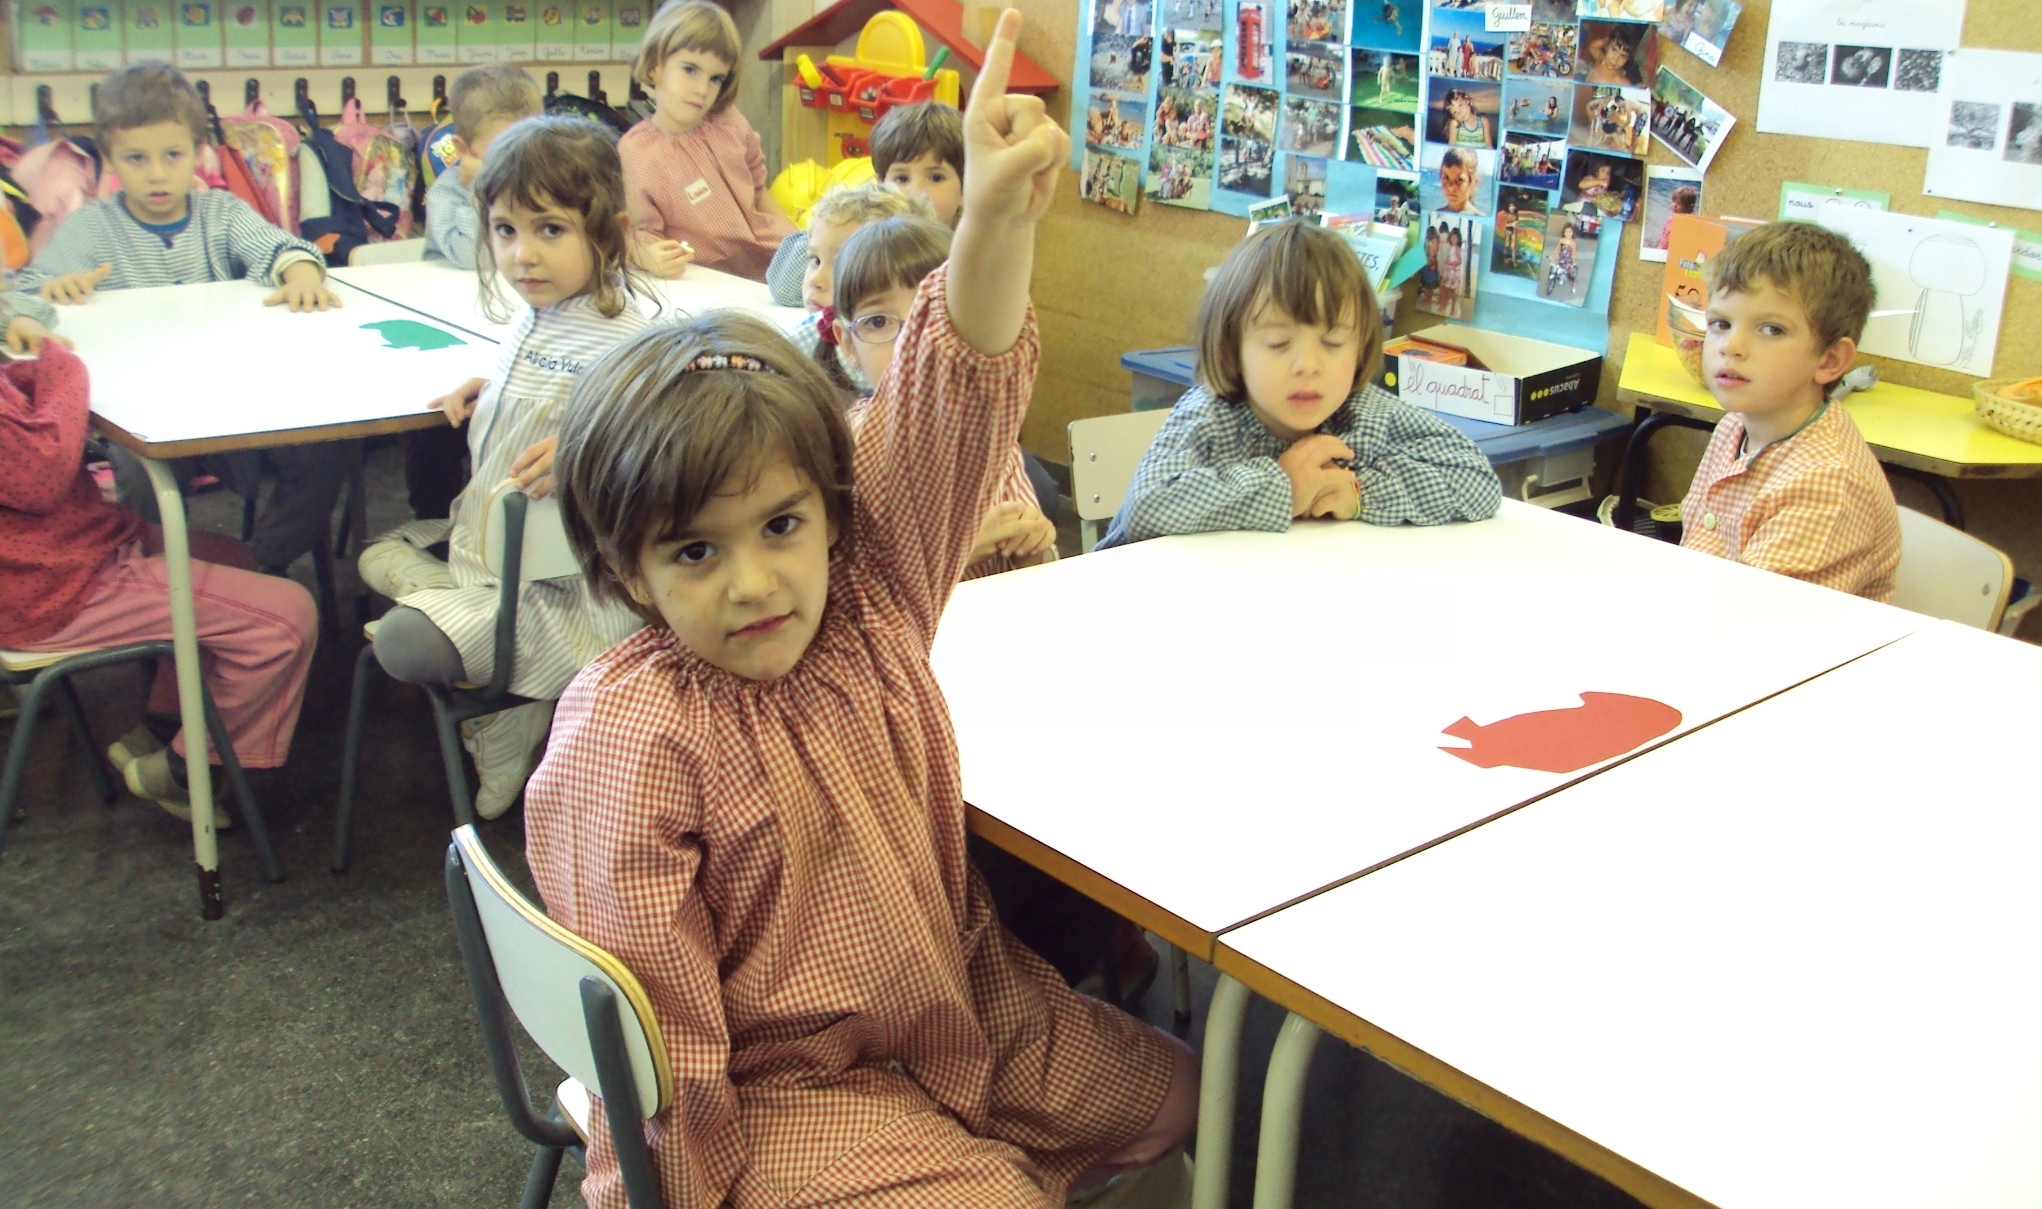
\includegraphics[width=9cm,keepaspectratio]{parvulari/img/foto3b.jpg}

Ara hem après a compartir les joguines,  a endreçar-les i a recollir les coses a poc a poc i respectant el material



\noindent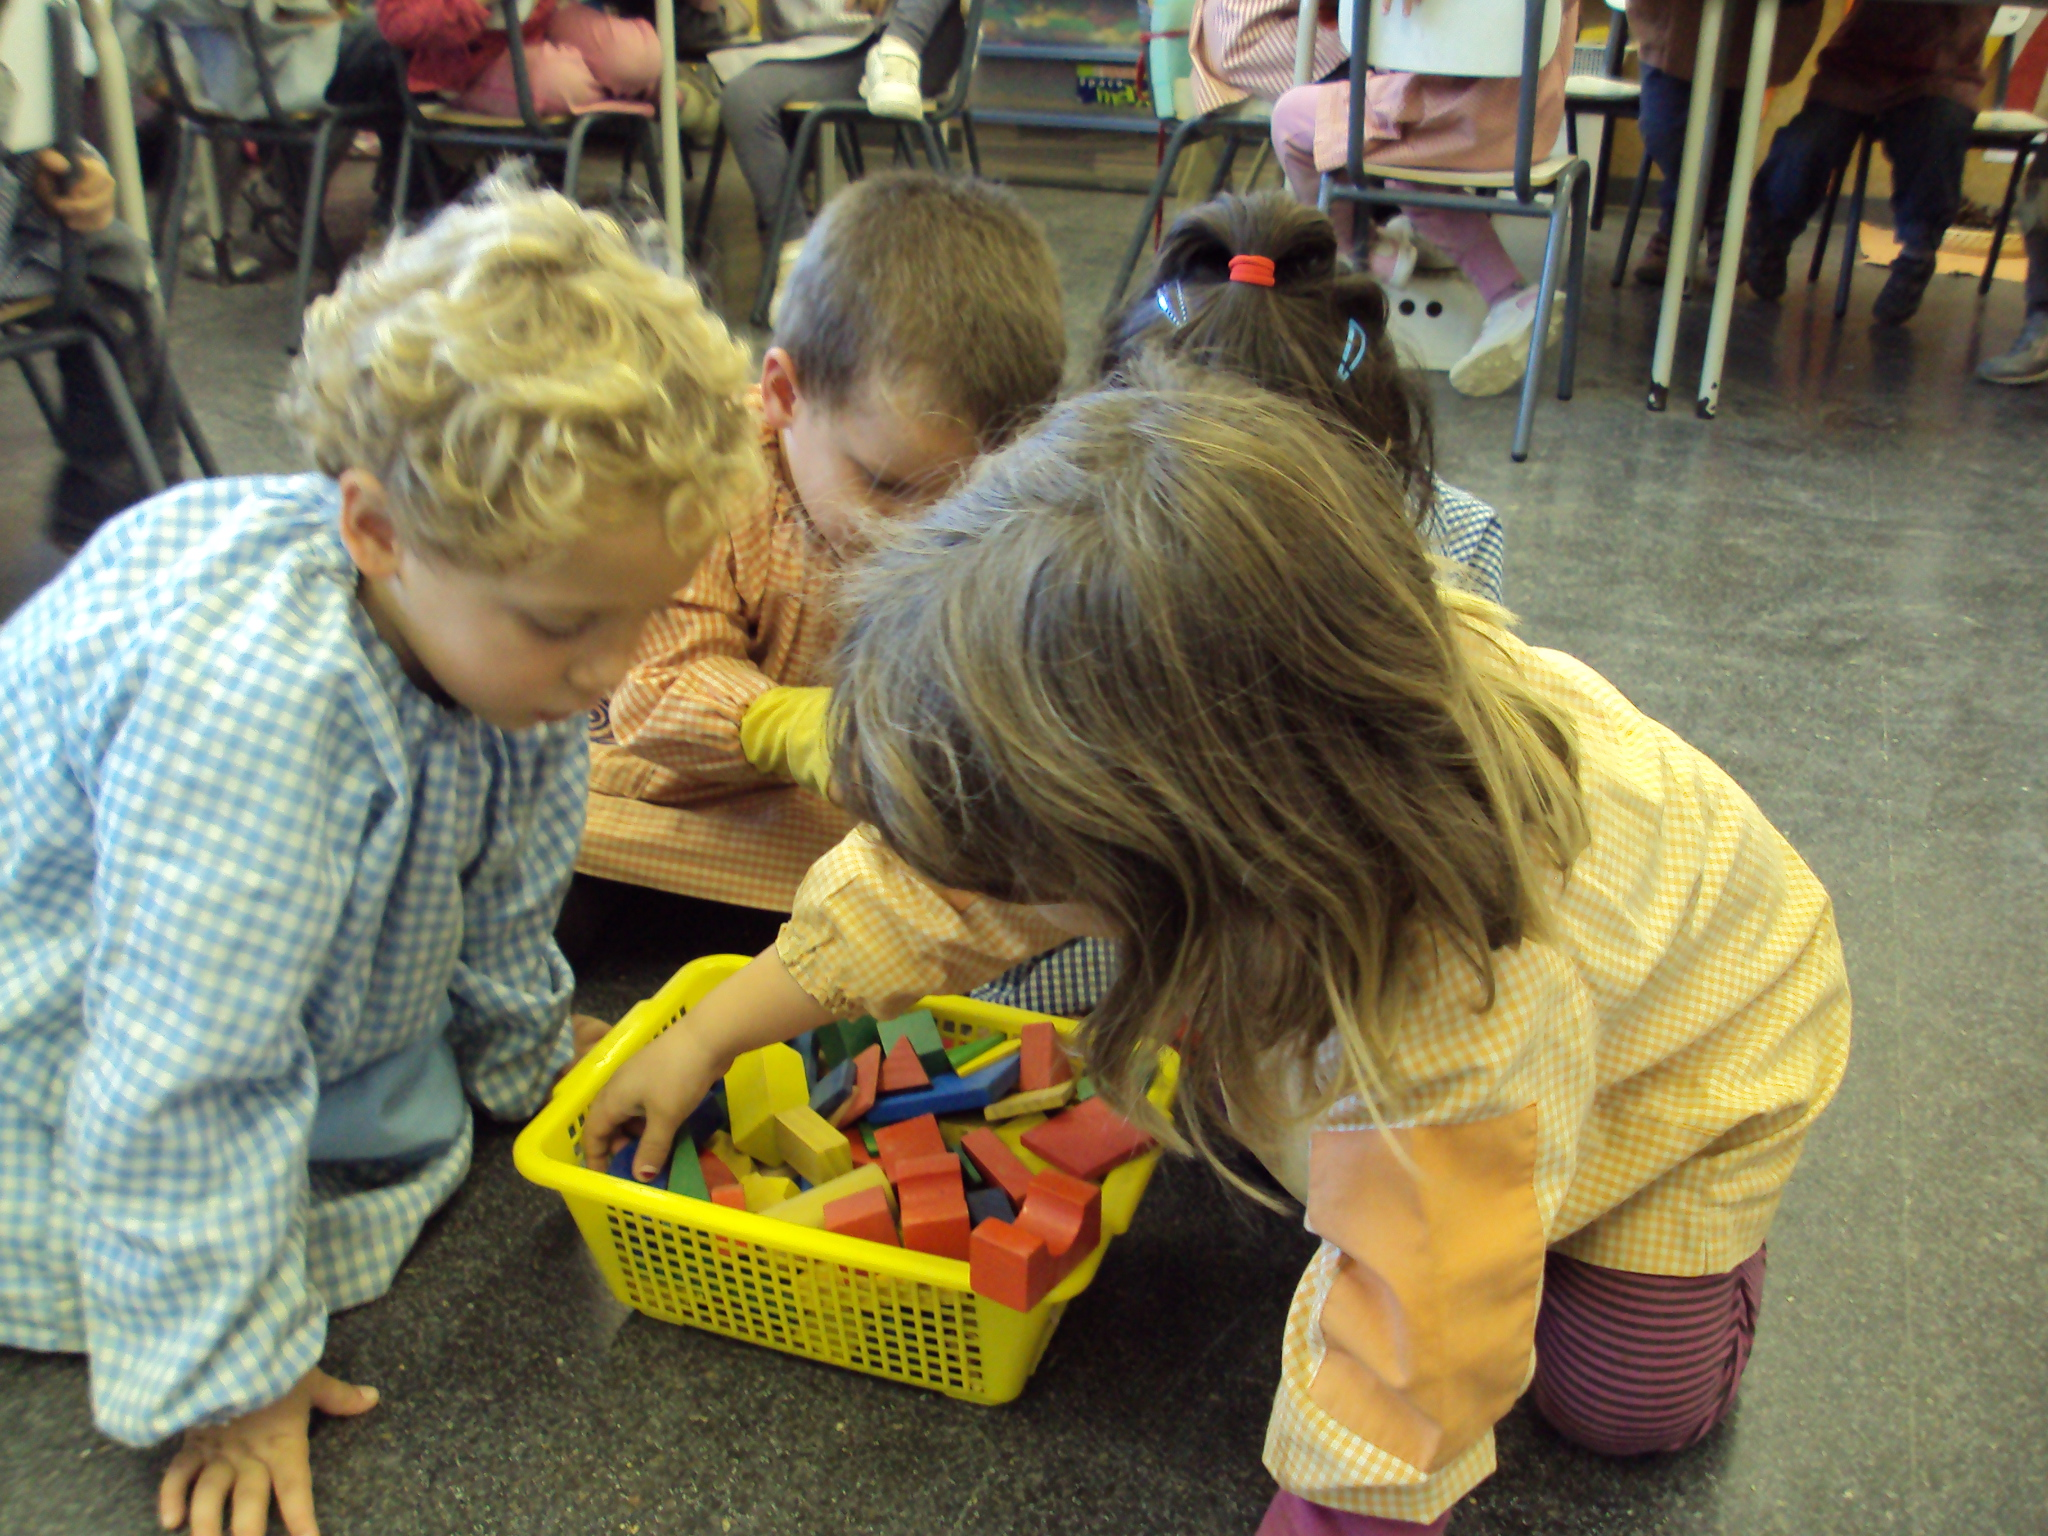
\includegraphics[width=9cm,keepaspectratio]{parvulari/img/foto4.jpg}

Els elefants expliquen: hàbits de treball

Nosaltres aprenem a escriure i a fer frases i la Toni ens posa deures per aprendre molt

\noindent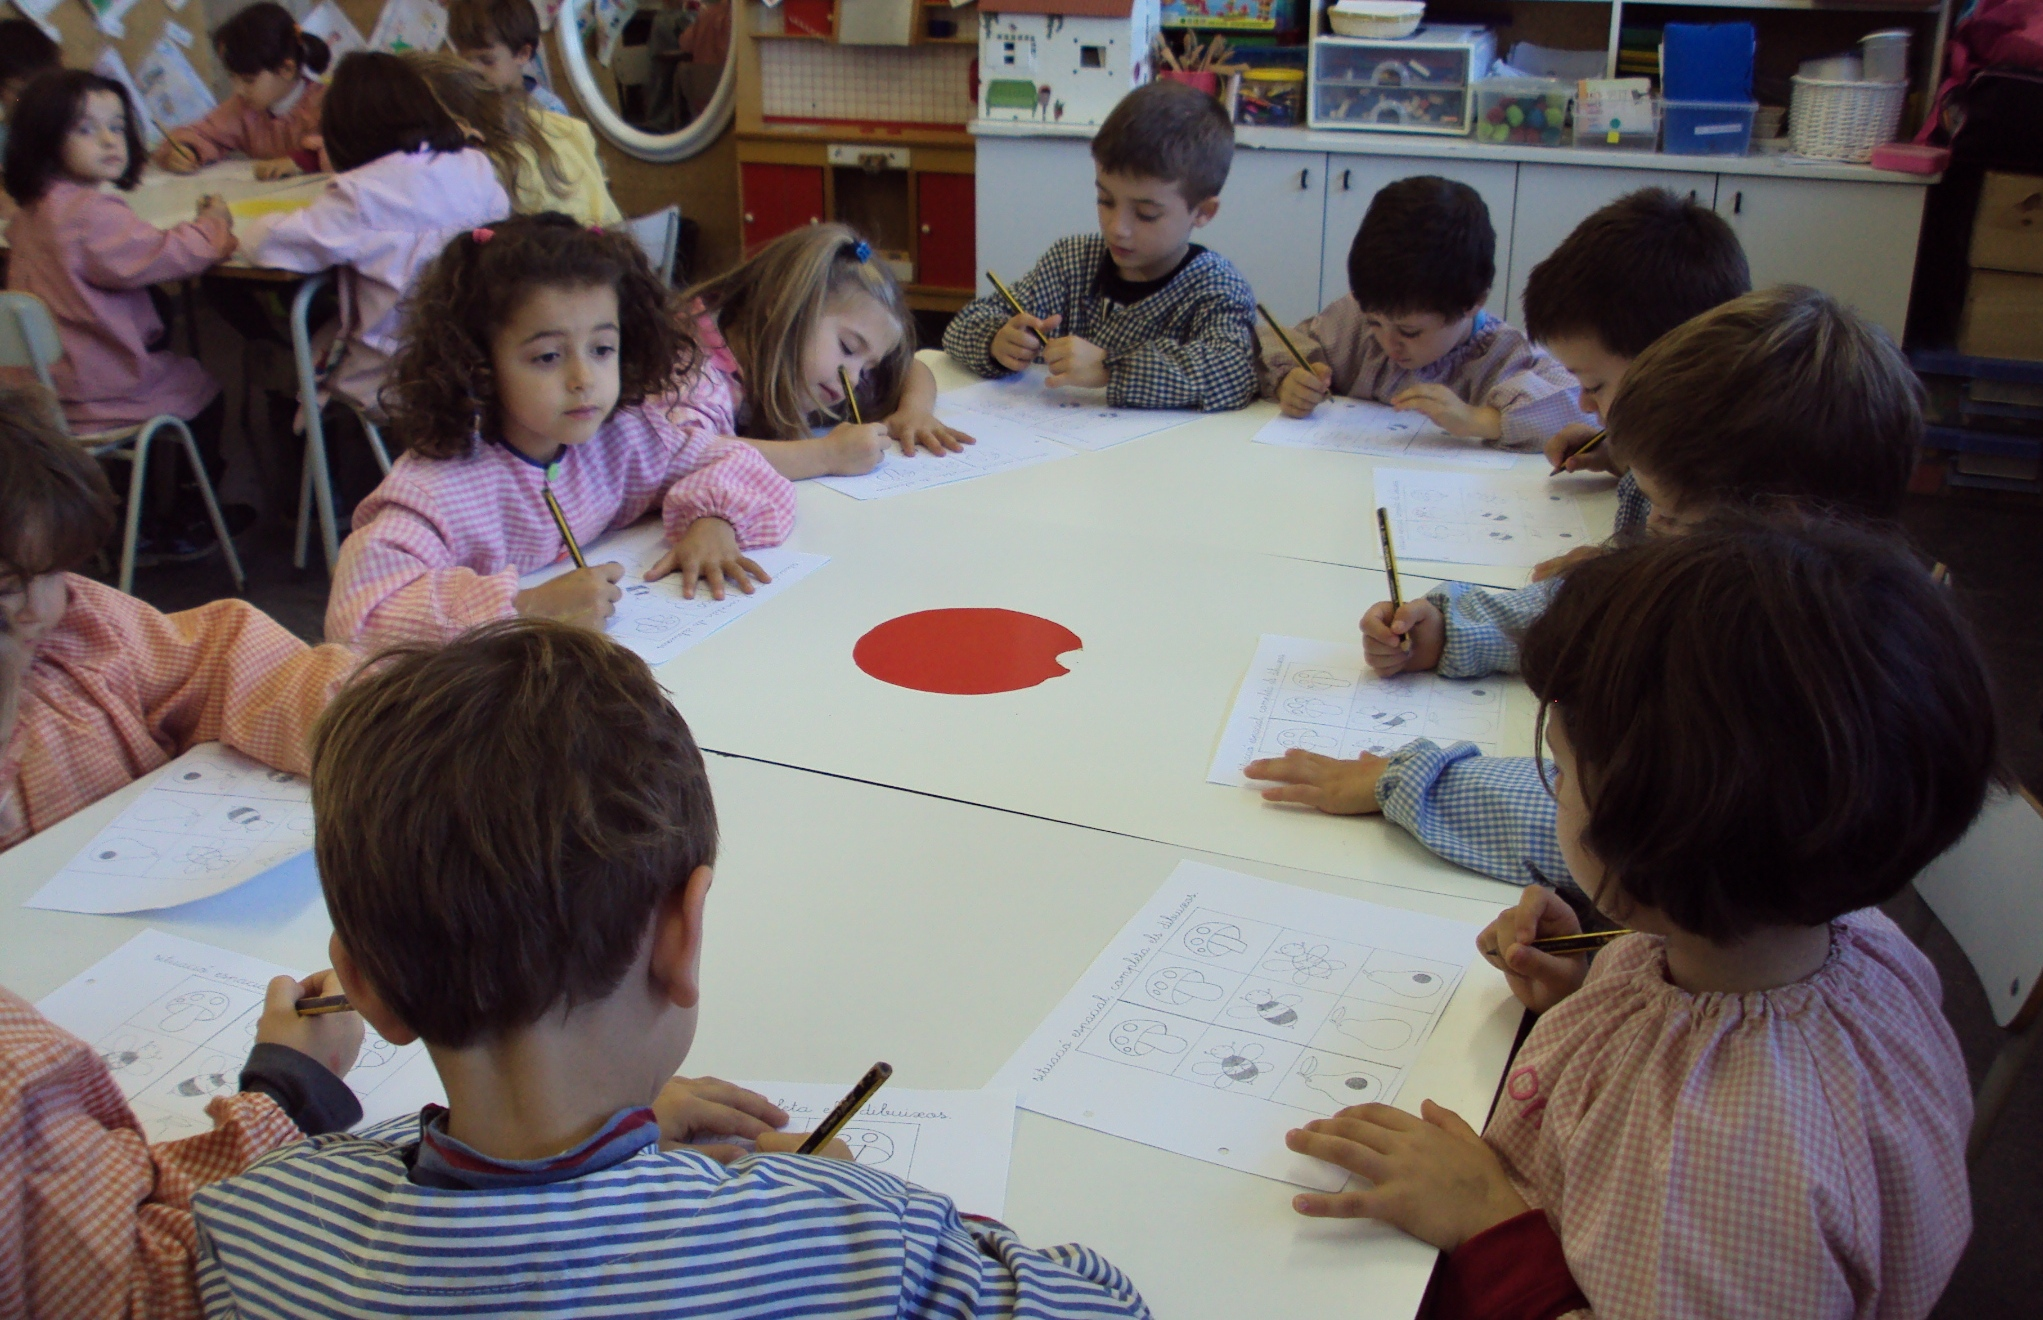
\includegraphics[width=9cm,keepaspectratio]{parvulari/img/foto5b.jpg}

Quan ens enfadem ara ja no ens barallem, parlem entre nosaltres perquè ja som molt grans

Fem quadern de matemàtiques, anem a l’aula d’informàtica i treballem amb la P.D.I.


\noindent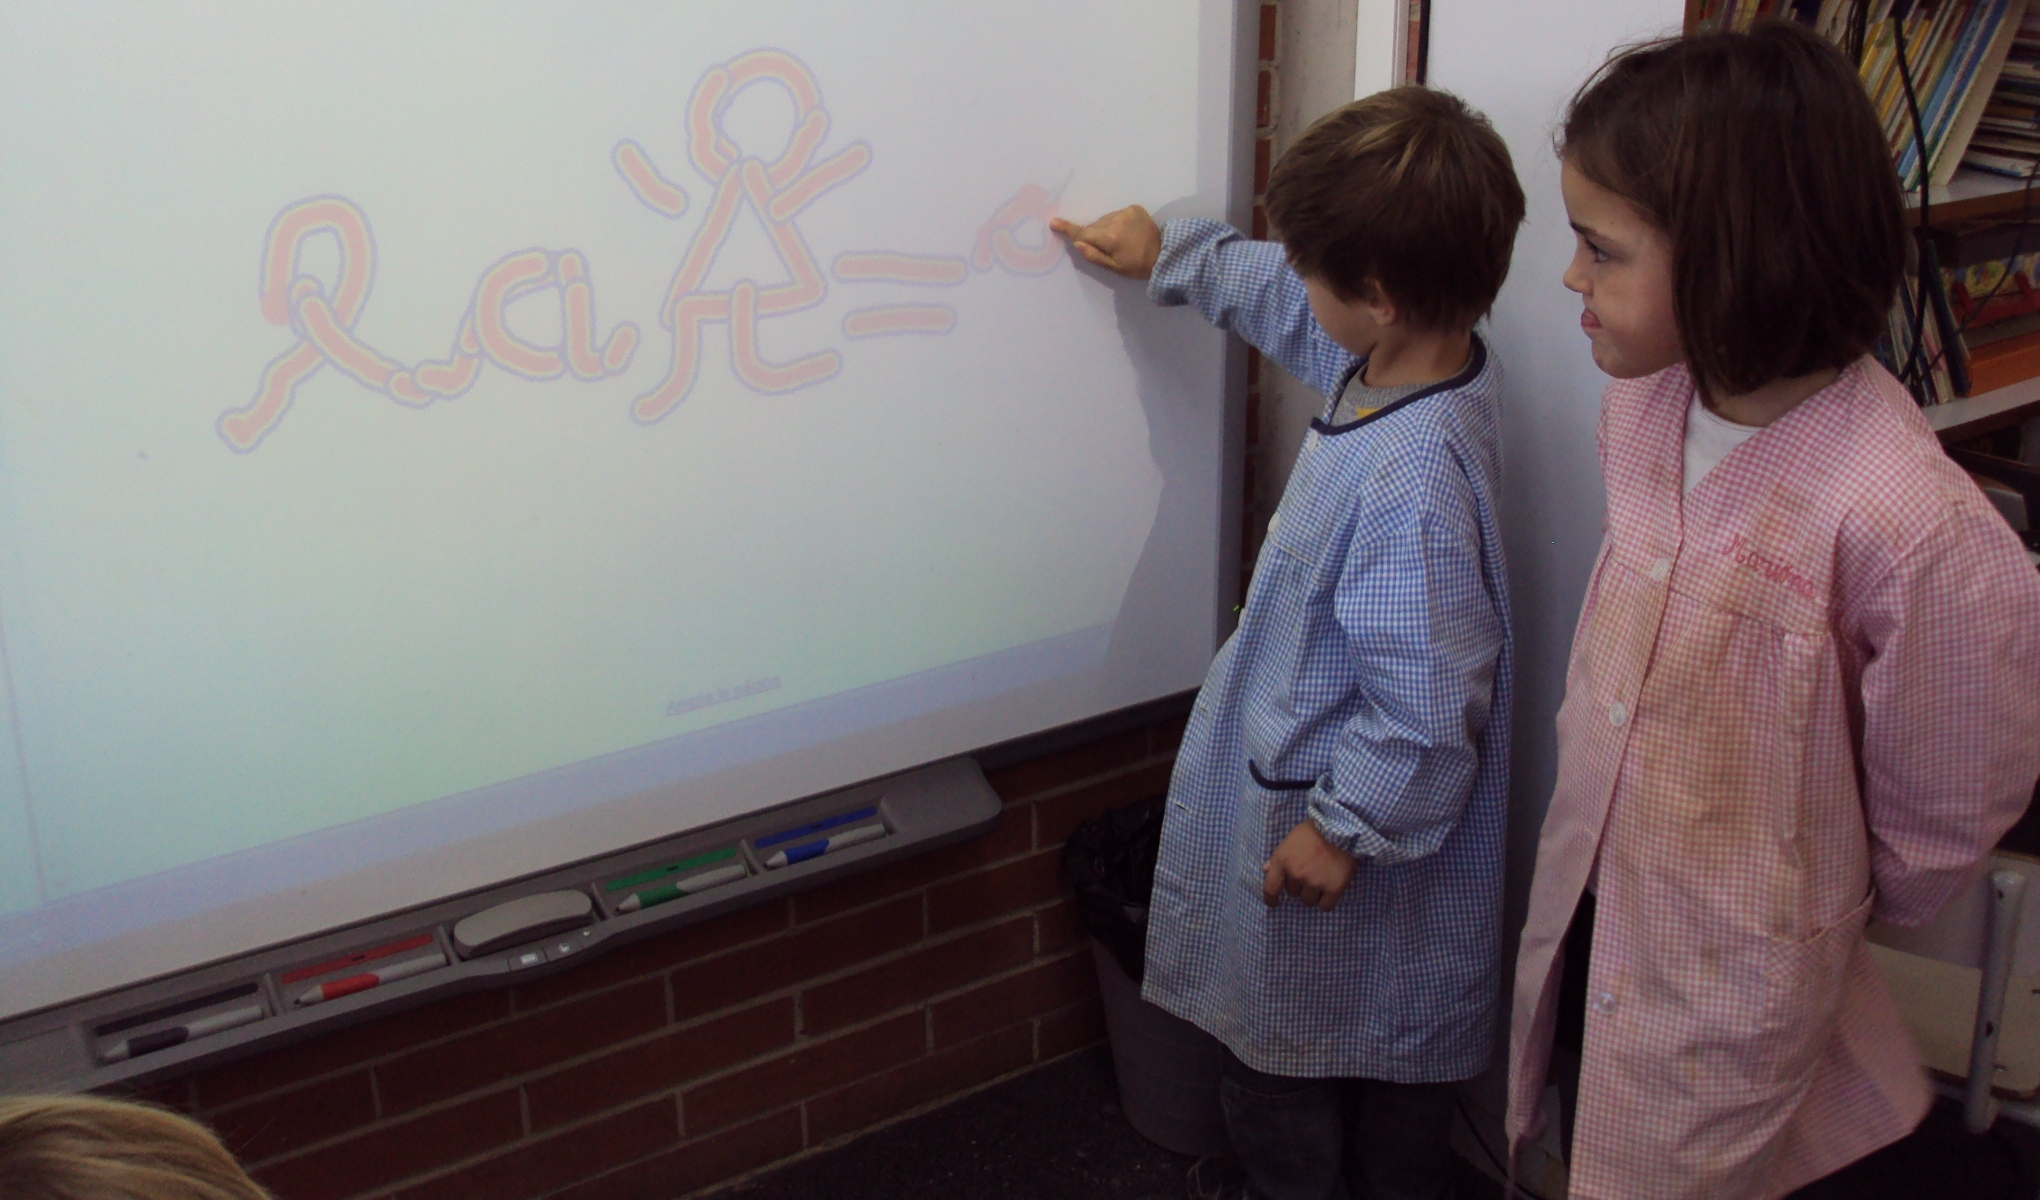
\includegraphics[width=9cm,keepaspectratio]{parvulari/img/foto6b.jpg}


Ara ja som grans i abans de contestar,  primer hem de pensar.


Tots aquests hàbits són  necessaris per a l’adquisició dels nous aprenentatges que assolirem al llarg de tota la nostra escolaritat.


\authorandplace{Les mestres de Parvulari}{Escola Solc}

\end{news}

\noindent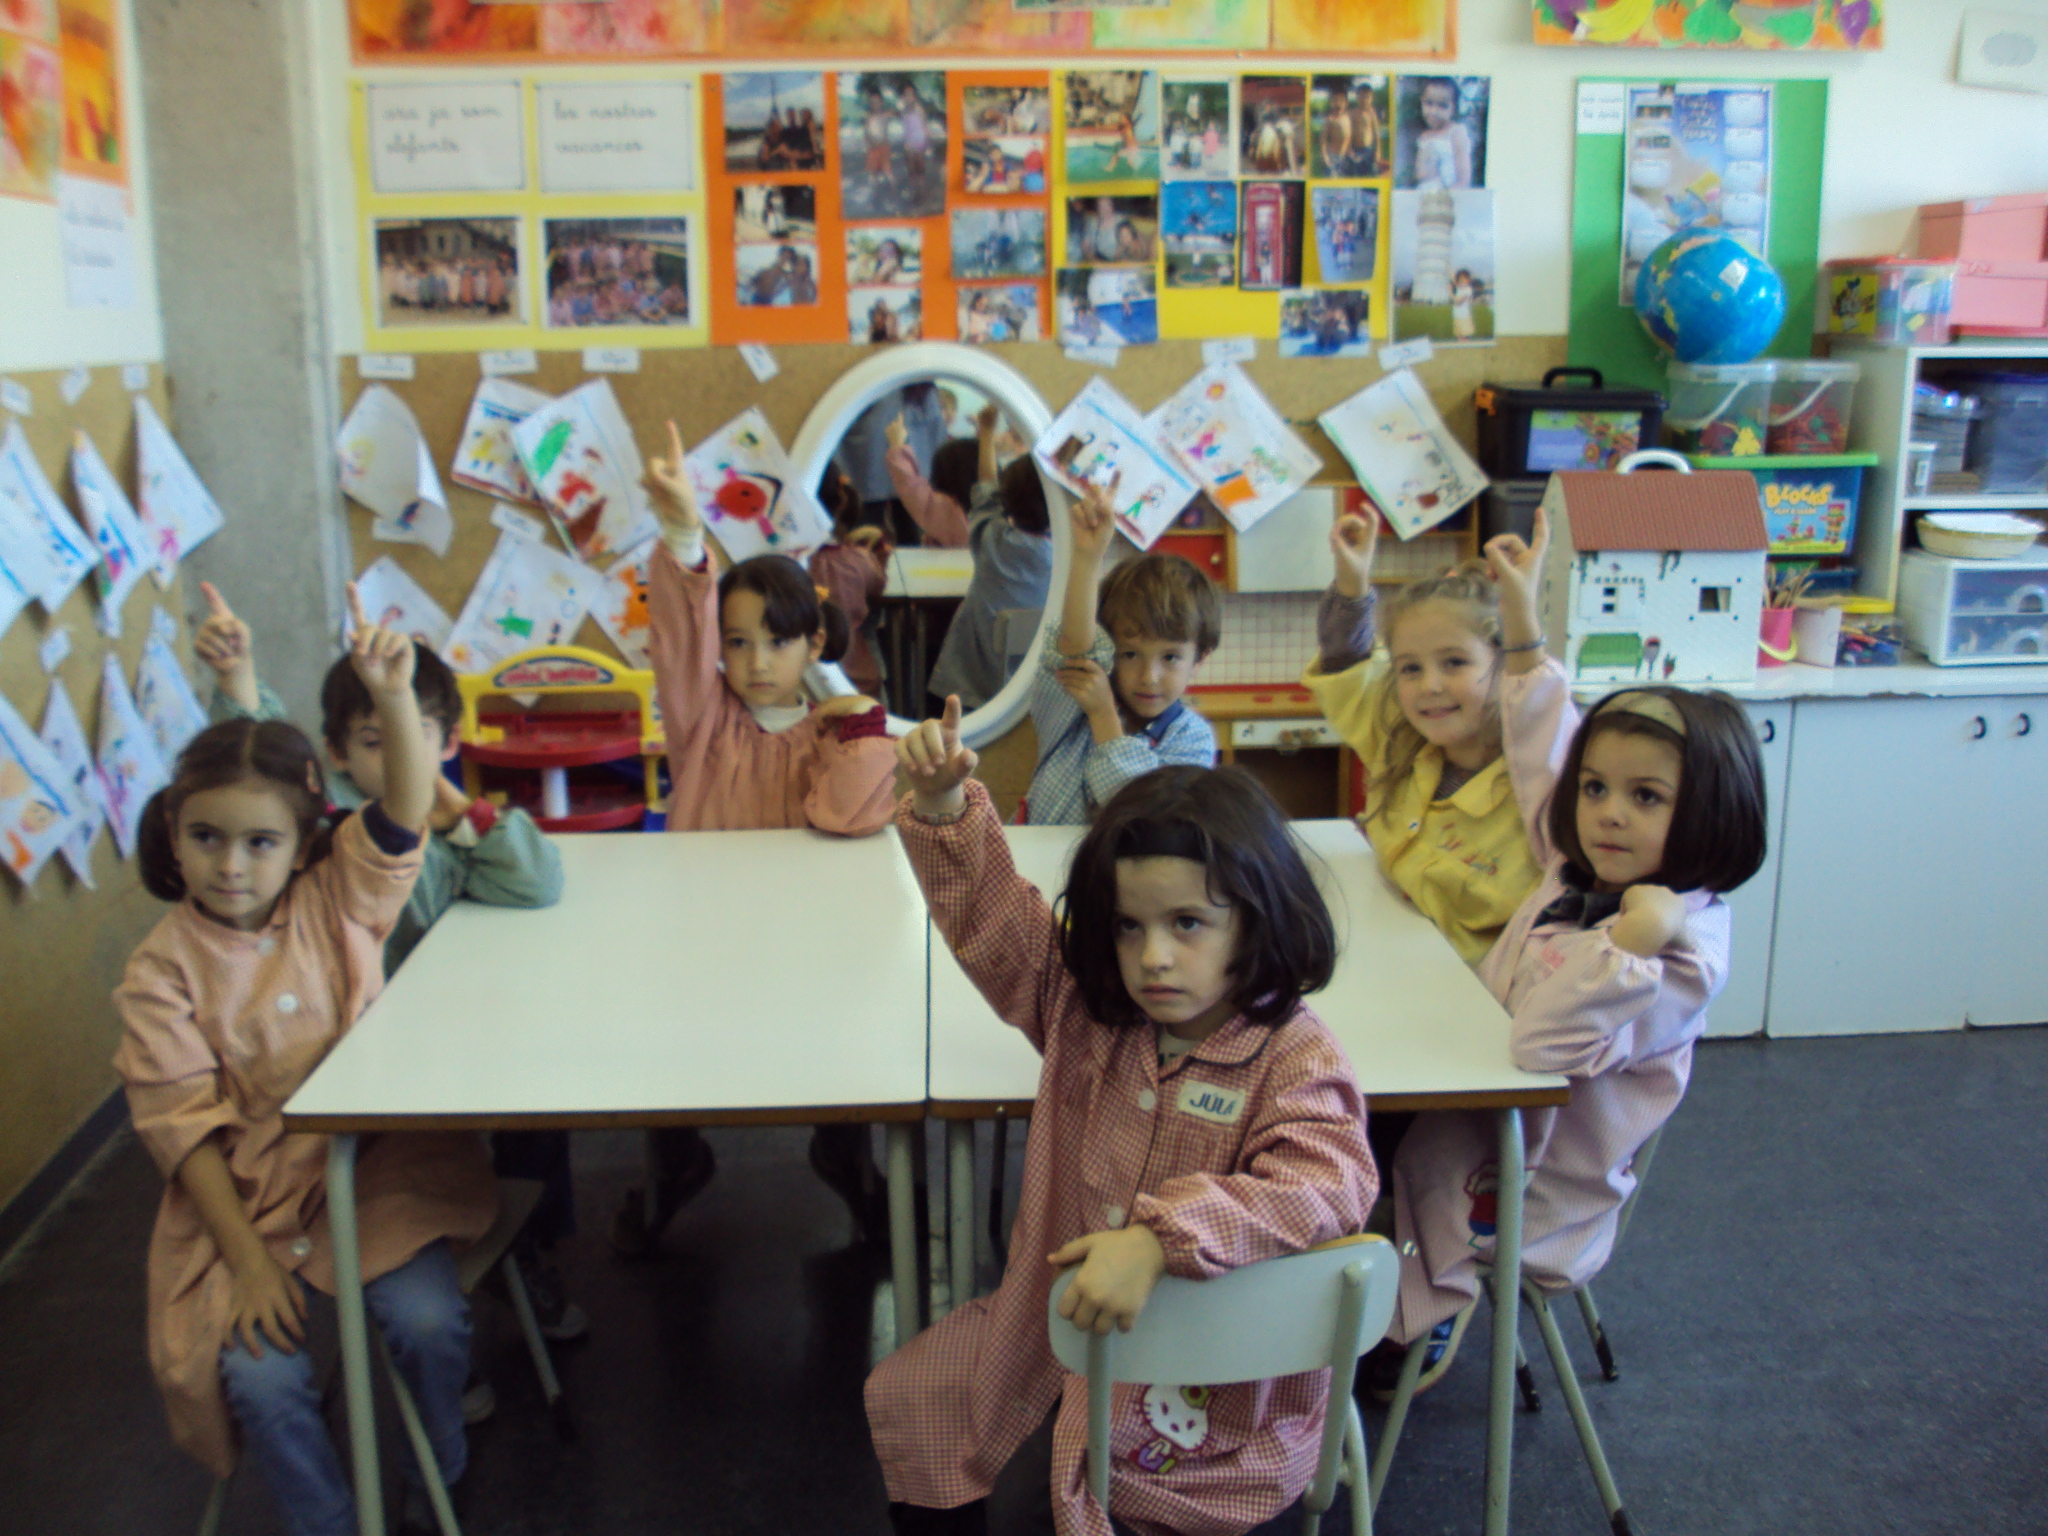
\includegraphics[width=12.5cm,keepaspectratio]{parvulari/img/foto7.jpg}




\newsection{Primària}
\definecolor{color}{rgb}{0.1 , 0.1 , 0.1}

\begin{news}
{2} %columnes
{El món de la Cèl·lula}
{El Dimecres 17 de març, els nens i nenes de 5è de primària de l’Escola Solc vam anar al CosmoCaixa a fer un taller de ciència que es diu “El món de la cèl·lula”}
{Primaria}
{5} %pagesof



Quan vam arribar al Museu vam conèixer a l’Eli i a la Irene, que van ser les monitores que ens van ajudar a fer les activitats. Hi havia dos tallers: un consistia en preparar mostres per observar pel microscopi i l’altre era mirar mostres ja preparades (orella de gos, testicle de rata,...). A la primera activitat, amb un tomàquet i una ceba havíem de fer les preparacions.
Després, un cop havíem fet tots dos tallers, vam estar una hora voltant pel CosmoCaixa. Jo vaig anar al Bosc Inundat, vaig tocar un bloc de gel gegant que hi havia, ...
M’ho vaig passar molt bé perquè el Museu de la Ciència és molt interessant.


\authorandplace{Albert Morales}
							{5è de Primària}

\noindent\includegraphics[width=9cm,keepaspectratio]{primaria/img/celula_DSC00655.JPG}

\end{news}

\newssep
\definecolor{color}{rgb}{0.1 , 0.1 , 0.1}

\begin{news}
{2} %columnes
{Elaboració dels titelles}
{Aquest curs, els nens de 5è de Primària estem preparant unes obres de titelles per representar-les al parvulari}
{Primaria}
{028} %pagesof




Primer havíem de portar un globus i un cilindre de cartró. Al voltant del globus enganxàvem paper amb cola. La cola feia que el cilindre s’ajuntés amb el globus. Quan es va eixugar el paper vam tornar a posar més capes de paper amb cola perquè ens quedés l’estructura més forta. Uns dies després, quan ja s’havia assecat, vam pintar el titella amb pintura blanca perquè no es veiés el diari. 

\columntitle{lines}
{Els titelles els fem nosaltres i les obres també les triem nosaltres}

Un altre dia el vam pintar amb els colors del personatge; per exemple, el meu  era un ós i el vaig pintar de color marró. Uns dies més tard, vam portar fil, agulla i tela per fer el vestit al titella. Tallàvem la tela en forma de vestit i després la cosíem. Fet això, el Ferran enganxava el vestit al cap amb belcro. Ja quedava fet el titella. També vam fer el guió de l’obra i un còmic per fer les fotografies. Aquestes ens serviran per fer un ``còmic digital" amb l’ordinador. Cap al juny representarem l’obra a parvulari i a la festa de final de curs podrem veure els ``còmics digitals".


M’agrada molt fer plàstica  sobretot, en aquesta ocasió, perquè hem treballat fent titelles i fent el ``còmic digital".

\authorandplace{Mar Garcia}
{5è de Primària}

\noindent\includegraphics[width=9cm,keepaspectratio]{primaria/img/titlles_513.jpg}

\end{news}
\definecolor{color}{rgb}{0.1 , 0.1 , 0.1}

\begin{news}
{2} %columnes
{Colònies de 1r i 2n de Primària}
%index: Colònies de Primària
{\noindent\includegraphics[width=18cm,keepaspectratio]{primaria/img/colonies_246.jpg}}
{Primaria}
{29} %pagesof

Dimarts 6 d’abril vam anar de colònies a una casa que es deia Can Putxet. Vam anar amb autocar  i era una mica lluny.

Quan vam arribar,  ens vam posar molt contents. Tenia un camp de futbol i una pista de tennis que semblava un camp de bàsquet. Vam estar jugant una estona, després vam dinar entrepans; un era de formatge i l’altre de pernil i, de postres, poma. Vam continuar jugant i va començar a ploure,. 

Vam entrar a la casa de dos en dos. A mi em va tocar amb el Joan, va voler dormir a dalt i jo vaig dormir a baix, tenia al Casi al davant i al costat l’Elena.

%\columntitle{lines}
%{També vam fer una excursió de tres quilòmetres i ens vam cansar molt}

Després vam fer unes activitats. La que més ens va agradar  va ser un joc d’equip. Els equips els vam fer segons els colors d’uns pitets  que ens van donar. Jo anava amb l’Alejandra, l’Elena, el Guillem T., el Gullem R., el Pol de primer, l’Aida i l’Oscar. Érem el color groc. Havíem de trobar 10 targetes d’animals. Només en vam trobar 8, perquè una se’ns va perdre i d’una altra ja  no en quedaven. Teníem un mapa per trobar els topants on buscar les targetes.

Per sopar hi  va haver sopa, truita de patates amb croquetes miniatura i per  postres iogurt. També vam fer una excursió de tres quilòmetres i ens vam cansar molt.

L’última nit vam fer un joc de nit, havíem de trobat tres claus: una al bosc, que era molt fàcil i la va trobar el Pol. L’ altra al camp, que va ser molt difícil i la va trobar l’Àlex. L’altra al riu, la va trobar l’Éric.

M’ho vaig passar molt Bé.

\authorandplace{Martina Tarrés Castellanos}{Primària}

\end{news}

\definecolor{color}{rgb}{0.1 , 0.1 , 0.1}

\begin{news}
{2} %columnes
{}
{}
{Primaria}
{029} %pagesof

%\vspace*{1cm}

El dimarts vam anar de colònies amb motxilles o maletes, les vam deixar al camp de futbol i vam començar a jugar. Després vam anar a la casa de can Putxet a veure-la per dintre. Vam començar per les habitacions, després pels lavabos. 

Vam tornar a les habitacions a fer el llit. Quan vam acabar, vam deixar la roba al calaix. Després vam jugar al camp de futbol un altre cop. Vam jugar a pilota. Després vam anar a passejar al camp, vam veure una riera.

Després vam tornar, quan vam arribar vam  anar a sopar. Després vam anar al llit a llegir i tot seguit a dormir. Quan ens vam llevar vam esmorzar i després vam fer una excursión que vam caminar tres quilòmetres. 

Vam berenar i, després, vam tornar a la casa de colònies, quan vam tornar vam sopar i després vam anar al llit, l’endemà marxàvem. Vam esmorzar, després arribava una altra escola, Vam jugar a una carrera de globus i també vam fer bombolles. 
Vam anar a dinar. I, després, vam marxar. 

\authorandplace{Màrio Ródenas Sistané}{Primària}


\end{news}
\definecolor{color}{rgb}{0.1 , 0.1 , 0.1}

\begin{news}
{3} %columnes
{Les Menines}
{}
{Primaria}
{30} %pagesof

\noindent\includegraphics[width=6cm,keepaspectratio]{primaria/img/picasso_ariadna.jpg}


Velázquez va ser un gran pintor del segle XVII, tot i que avui en dia les seves obres d’art són molt conegudes. Ell
 va ser l’autor de “Les Menines” que està exposat al museu del Prado, a Madrid. Si observem bé el quadre podem veure-hi el seu autor; al fons hi ha un mirall on s’hi pot veure Felip IV i Mariana d’Àustria, al seu costat José Nieto, prop de Velázquez hi ha una menina, al mig hi ha la infanta Margarida, al seu costat hi té una altra menina, també hi ha una nana, un nan, un senyor i una monja. 


Pablo  Picasso, també un gran pintor del segle XX, va imitar  “Les Menines” a la seva
manera, és a dir,  amb formes geomètriques, amb punts, amb carbonet, va afegir elements, personatges, etc. Va fer unes 58 versions sobre aquest quadre. 


A la nostra escola, els alumnes de 5è i de 6è vàrem fer un treball sobre “Les Menines” abans de la visita al museu Picasso.
Vàrem observar l’original i algunes de les moltes versions de Picasso. Després de parlar-ne, vam dibuixar l’obra a la nostra manera. Per exemple, amb pals, estil modern, còmic, puntillisme,...  En fi, tothom  va fer el seu estil i van quedar  tots molt bonics.

\noindent\includegraphics[width=6cm,keepaspectratio]{primaria/img/picasso_conrad.jpg}

\authorandplace{Guillem Morales}{6è de Primària}

\end{news}

\newssep
\definecolor{color}{rgb}{0.1 , 0.1 , 0.1}

\begin{news}
{2} %columnes
{Visita al museu Picasso}
{}
{Primaria}
{030} %pagesof


El dimarts 23 de març vam anar al Museu Picasso, que es troba al Barri Gòtic de Barcelona, al carrer Montcada, que és un carreró estret, antic i sense cotxes. Allà vam aprendre moltes coses d’aquest pintor malagueny.  

Quan hi vam entrar jo em vaig sentir com un veritable artista. Ens van explicar la vida de Pablo Picasso, la del seu pare (José Ruiz) i la de la seva mare (Maria Picasso). Ens van dir que Picasso va començar a dibuixar amb carbonet, que va presentar el quadre de “La dona malalta” a la universitat de Belles Arts de Madrid, que el seu pare era  professor en una universitat que es deia “Llotja”. També ens van ensenyar quatre estils de la seva pintura: carbonet, l’època blava, figures geomètriques i el puntillisme. 

Vam veure el quadre “La dona malalta” que, segons ens van explicar,  representava una dona molt malalta al llit amb un metge prenent-li el pols i una monja oferint-li un got d’aigua, aquesta portava un nadó a les mans. En realitat, el metge era el pare del Picasso, la dona malalta, una pidolaire, el nadó, el fill de la pidolaire i, la monja, era un amic de Picasso.

A més a més de veure els quadres més importants d’aquest pintor, em va agradar poder llegir la seva vida, que estava escrita a diverses parts del museu. 

\authorandplace{Óscar Redondo Mora}
				{6è de Primària}

\noindent\includegraphics[width=8cm,keepaspectratio]{primaria/img/picasso_julia.jpg}

\noindent\includegraphics[width=8cm,keepaspectratio]{primaria/img/picasso_raquel.jpg}

\end{news}
\definecolor{color}{rgb}{0.1 , 0.1 , 0.1}

\begin{news}
{2} %columnes
{La Bombeta}
{}
{Primaria}
{029} %pagesof

\noindent\includegraphics[width=9cm,keepaspectratio]{primaria/img/bombeta.png}

L’invent de la bombeta s’atribueix a Thomas Alva Edison que va presentar la patent  el 21 d’octubre de 1878. Està formada per un filament de wolframi molt primet situat a l’interior d’una “ampolla” de vidre que s’ha omplert posteriorment d’un gas inert o bé se li ha fet el buit. A la part de sota de la bombeta hi ha una part metàl·lica on s’hi troben totes les connexions elèctriques. Aquesta part metàl·lica, normalment té una una rosca que permet caragolar la bombeta al portalàmpades. La bombeta elèctrica també s’anomena làmpada incandescent.  De tota l’energia que consumeix la bombeta, només el 10\% es converteix en llum; la resta, es transforma en escalfor, llum ultraviolada i llum infraroja. 
La bombeta és un dels objectes més utilitzats des de la seva invenció, ja que tots en tenim, com a mínim, una a casa.

\authorandplace{Conrad Galli}{6è de Primària}

\end{news}

\newssep
\definecolor{color}{rgb}{0.1 , 0.1 , 0.1}

\begin{news}
{2} %columnes
{L'ós}
{}
{Primaria}
{029} %pagesof

\noindent\includegraphics[width=9cm,keepaspectratio]{primaria/img/os.png}

Els óssos són omnívors, ara bé, l'ós polar, a causa de la manca d'altres fonts d'aliment, té una dieta quasi exclusiva de carn. Amb els seus pesats cossos i les seves poderoses mandíbules, els óssos es compten entre els majors carnívors que viuen a la Terra. Un mascle d'ós polar pot pesar més de 600 kg i pot aconseguir 1,60 m. d'altura quan es posa de quatre potes. Es desplacen amb uns moviments pesats tot  recolzant tota la planta dels peus. Posseeixen orelles curtes i cua rudimentària. Tenen una dieta variada i, tot i la seva temible dentadura, molts d'ells mengen fruits, arrels i insectes, a més de carn. 
Contràriament al que pot semblar a primera vista, ha estat molt debatut si els pandes són o no óssos, encara que els últims exàmens genètics suggereixen que els grans pandes sí que ho són.


L'ós era un animal sagrat al nord d'Europa, on era el rei del bosc. Se'l representa en els mites i llegendes com l'animal més semblant a l’home; fins i tot, arribava a tenir relacions amb dones humanes (fet pel qual l'església cristiana el va degradar com a associat al dimoni a partir de l'any mil). El nom propi Úrsula deriva directament de l'ós. Representa els països de Finlàndia i Rússia i és un emblema de la comunitat de Madrid.

\authorandplace{Arnau Ruiz}{6è de Primària}




\end{news}
\definecolor{color}{rgb}{0.1 , 0.1 , 0.1}

\begin{news}
{4} %columnes
{L’Ot i els alumnes de 3r de Primària}
% index: L'Ot i 3r de Primària
{}
{Primaria}
{15} %pagesof


\noindent\includegraphics[width=4.5cm,keepaspectratio]{primaria/img/ot_imagen.jpg}

\bf L’Ot va a Egipte

\rm
Un dia l’Ot va anar amb l’escombra màgica de passeig i va arribar a Egipte, i mentre volava es va trobar a tres àrabs. Es veia que aquells senyors volien anar a  algun lloc. Finalment l’Ot va dir unes paraules màgiques: PLOP!! I, de sobte, l’escombra es va convertir en una catifa voladora. Així van poder pujar els tres àrabs que van quedar contents i resant cap al poble.

                                      Eloi Ibáñez           


\noindent\includegraphics[width=4.5cm,keepaspectratio]{primaria/img/ot_imagen_001.jpg}

\bf L’Ot i la senyora globus

\rm
Hi havia una vegada un bruixot que es deia Ot i també una princesa anomenada Berta. Un dia la Berta era en el seu castell i va aparèixer l’Ot i li va dir: 
-   Hola princeseta, estàs bé? 
Sí, va dir la Berta; i tu què fas per aquí?
Volia saludar-te i  veure com estaves.
Doncs estic molt bé.
Aleshores, l’Ot va agafar la Berta per les cames i la va inflar com un globus i va fer PLOP! Llavors va posar-li una corda i va agafar-la tot caminant... I així és la història de l’Ot i la Berta.
     
                                                           Adriana Bosch


\noindent\includegraphics[width=4.5cm,keepaspectratio]{primaria/img/ot_img025.jpg}

\bf L’Ot i les amigues de la Berta

\rm
Un dia l’Ot s’estava banyant i quan va acabar de banyar-se va agafar la tovallola i es va eixugar. Va obrir la porta i va trobar les amigues de la Berta. Aleshores, perquè no el veiessin, va fer ús de la seva màgia i va caminar pel sostre. Va anar a l’altra porta i les amigues de la Berta no el van veure.

                                                                Irene Cuadra

\noindent\includegraphics[width=4.5cm,keepaspectratio]{primaria/img/ot_img022.jpg}

\bf La gran barba

\rm

Una vegada hi havia un bruixot que es deia Ot i anava cap a la perruqueria. Llavors va dir: - no tinc cabells perquè me’ls tallin, doncs m’hauré de tallar el bigoti i això no m’agradaria, seria imperdonable. Aleshores, com que era un bruixot, va fer-se aparèixer una gran barba a la barbeta. Va entrar i no va sortir fins al dia següent, però no li van tallar la barba sinó el bigoti. Va sortir enfadat; en canvi,  de content , gens ni mica.

                                                             Ferran Corral 


\end{news}
\definecolor{color}{rgb}{0.1 , 0.1 , 0.1}

\begin{shortnews}
{3} %columnes
{Ressenyes de llibres}
{}
{Primaria}

\shortnewsitem{La marmota inventora}
{
Autor: Enric Larreula / Rita Culla.   Editorial: La Galera 

Hi havia una vegada una marmota molt llesta que un dia va fer un invent, una bufanda. La va tallar a trossets i la va regalar a totes les marmotes. La bufanda la va fer servir per dormir. La marmota vivia en unes muntanyes molt altes anomenades els Alps.

A mi m’ha agradat molt perquè tracta d’invents i de marmotes.
									
Biel Castro, 1r de Primària
}

\shortnewsitem{La campaneta de plata}
{
Autor: Conte popular.   Editorial: Susaeta

En una torre hi vivia la mare dels vents, que tenia tres fills: el vent del Nord, la Brisa i el vent de Llevant. Quan es van fer grans van viatjar per diferents mons, i van deixar una campaneta de plata a la mare per si els volia cridar.  Com que la mare es sentia sola, va tocar la campaneta per reunir els tres germans, però de tant vent, el poble es pensava que a la torre hi vivia una bruixa.

M’ha agradat aquest llibre perquè la mare reuneix els seus fills tocant la campaneta.
									
Aida Perez, 1r de Primària
}

\shortnewsitem{Pinotxo}
{
Autor: Carlo Collodi      
\noindent\includegraphics[width=4.5cm,keepaspectratio]{primaria/img/llibres_pinocho.jpg}

Un dia un fuster anomenat Gepetto va construir un titella, que va anomenar  “Pinotxo”. Va desitjar que  ell tingués vida. A la nit va venir una fada i va fer que el titella cobrés vida. Pinotxo es va sorprendre molt perquè podia parlar, caminar, menjar, anar a l’escola, etc. Pepito Grillo era la consciència de la marioneta, que el va ajudar a ser conscient del que feia. 

Em va agradar molt perquè la fada va fer màgia i a mi això m’agrada molt. Aquest llibre el recomano perquè és molt divertit, emocionant i hi passen moltes aventures.

Pol Hernández,  2n de Primària
}

\shortnewsitem{El mag Merlí}
{
Autor: Llegenda Popular.    Editorial: Susaeta  

Un nen anomenat Grill vivia en un castell a Alemanya. Un dia en Grill amb un amic que es diu Key van anar a caçar, però com que en Grill era novell  en la caça, va caure des d’un arbre a sobre d’en Key fent que llancés una fletxa al cel; en veure el que havia fet, en Grill li va dir que aniria a cercar la fletxa. En Grill anava cercant la fletxa quan, de sobte, va veure la fletxa en una branca, l’anava a agafar,  va relliscar i va caure en una cabana on hi vivia en Mag Merlí.  Li va dir que havia de  tornar al castell...    

A mi el que més m’ha agradat és quan llençava la fletxa. I,quan estan caçant, hi ha un dibuix que em va agradar molt.

Damià Rubió ,  2n de Primària
}

\shortnewsitem{La Xola i els lleons}
{
Autor: M. Dolors Alibés.   Editorial: Cruïlla

És una gossa que es diu Xola i que es pensa que es un lleó, llavors l’imita. El seu amo,  en Marc, té un amic que investiga la selva, llavors l’amic porta un llibre de lleons a casa la Xola i se’l deixa. La gosseta, com que està tan interessada en els lleons, l’agafa i el llegeix i descobreix que els lleons no són tan fantàstics com ella creia i ja no vol ser un lleó. I ara és una gosseta petonera com abans era.

M’ha agradat molt perquè és molt misteriós i no saps què passarà. També perquè mai  pots decidir ser un lleó si no saps res sobre ells.

Andrea Amador Alcaina,  2n de Primària
}

\shortnewsitem{Geronimo Stilton. Les entranyes de les rates pudents}
{
Autor: Geronimo Stilton.   Editorial: Destino

Aquest llibre parla que Ratalona comença a fer molta pudor. Una nit, de sobte,  de les clavegueres surten globus pudents. En Gerónimo baixa a les clavegueres per esbrinar què feia tanta pudor. Caminant per les clavegueres, arriba a Ratcity, la ciutat de les rates. Hi ha una rata que es diu Clavegueram que és una mica dolenta, i quan arriba a Ratcity s’enamora del Xafarot, l’amic d’en Geronimo i es vol casar amb ell. En Xafarot i en Geronimo agafen una moto d’aigua i s’escapen.

Ens ha agradat molt perquè aquest llibre és de misteri. També ens agraden molt les aventures d’en Gerónimo Stilton.

Eloi Banyes, Ferran Corral i Roger Guarro, 3r de Primària
}


\shortnewsitem{La Tanga i el gran lleopard}
{
Autor: Roberto Malo i Fco Javier Mateos.  Editorial: Comanegra

La Tanga és una noia que viu en un poblat al cor de la selva. En el poblat hi ha un mag que es diu el Gran Bruixot i que té poders màgics. Un bon dia, un lleopard ferotge i cruel va menjant-se tots els animals del poblat. A partir d’aquell succés van començar a patir fam, i el Gran Bruixot va intentar aturar e lleopard, però no va funcionar. A la nit es va posar una màscara per transmetre un missatge als ciutadans. I va dir a tot el poblat que el dia següent tothom que volgués enfrontar-se al lleopard es presentés, però no va aparèixer ningú, excepte la Tanga. Llavors el Gran Bruixot li va donar un ganivet de fusta de banús... 

Ens ha agradat molt perquè aquest llibre és una aventura molt divertida i perquè ens agrada molt la màgia i el Gran Bruixot en fa molta.

 Pablo de Quadras i Eduard Tenas,  3r de Primària
}


\shortnewsitem{El zoo d’en Pitus}
{
Autor: 	Sebastià Sorribas.  Editorial: La Galera

\noindent\includegraphics[width=4cm,keepaspectratio]{primaria/img/llibres_pitus.jpg}

El Pitus té una malaltia. Només el pot curar un metge molt famós de Suècia. Els seus amics, el Tanet, el Manelitus, en Cigró, en Juli, en Fleming i la Mariona van tenir una gran pensada: com que a en Pitus li agradaven molt els animals, van decidir fer un zoo per a ell.

M’ha agradat molt l’argument d’aquest  llibre.

Roser Pérez, 4t de Primària
}

\shortnewsitem{Tina superbruixa. L’aniversari d’en Pitus}
{
Autor: Knister   Editorial: Bruixola

\noindent\includegraphics[width=4cm,keepaspectratio]{primaria/img/llibres_fada.jpg}

Aquesta és una de les emocionants històries de la Tina. És l’aniversari d’en Pitus i està molt emocionat i vol fer una súper festa, però el seu pare està de viatge i la seva mare en un curs. Ve la seva tieta, que és una mica bleda  amb els nens. A la Tina i al Pitus els tracta com a nadons. Quan arriben els convidats, la tieta Elisa es queixa i es queixa fins que la Tina fa un dels seus encanteris i... Plaf! La tieta s’adorm.

M’ha agradat perquè és molt divertit, és una mica curt, però val la pena. És entretingut i el recomano a tothom.

Ariadna Vera, 4t de Primària
}

\shortnewsitem{Els rebels de la cabana}
{
Autor: David Nel·lo.   Editorial: Cruïlla

Va d’un grup de nens que tenen feta una cabana a dalt d’un arbre i l’alcalde vol construir un aparcament al Prat, tallaran l’arbre on hi ha la cabana. La Margot, que és la que mana, vol negociar amb ell perquè no tallin l’arbre, però l’alcalde diu que no. Aleshores, els nens van dir que si no negociaven, no baixarien de la cabana. 

És molt divertit perquè els nens són molt atrevits ja que es queden una nit de pluja a la cabana. Jo el recomano perquè és molt emocionant.

Aina Boronat, 5è de Primària
}

\shortnewsitem{La tribu de Camelot}
{
Autora: Gemma Lienes.    Editoria: Empúries

El Papagueno, el canari de la veïna de la Carlota ha desaparegut i la tribu passa moltes aventures amb un llibre de màgia que els ajuda a retornar en Papagueno a la veïna de la Carlota.  

Aquest  llibre m’ha agradat molt perquè hi ha moltes aventures i és molt intrigant per saber qui ha raptat Papagueno. M’entretenia a trobar els dracs que hi havia amagats a moltes pàgines, també eren molt divertides les olors i les tintes.  
Paula Claver, 5è de Primària
}

\shortnewsitem{Pocahontas}
{
Autor: Walt Disney.   Editorial: Beascoa

La història comença quan va arribar una expedició de navegants a la terra dels indis.
L’objectiu era trobar or i enriquir-se. Casualment, en John coneix la Pocahontas i se n’enamora. Al pare de la Pocahontas  això no li agrada ja que volia que es casés amb en Kocum. En una baralla per la Pocahontas, mor en Kocum i fan presoner en John. Els amics d’en John corren a salvar-lo amb les escopetes...

És una història d’amor i d’aventures i a mi m’ha agradat molt!

Eva Llovera, 5è de Primària.
}


\shortnewsitem{La meravellosa medicina d’en Jordi}
{
Autor: Roald Dahl.   Editorial: Empúries

En Jordi és un noi que  sempre ha d’estar cuidant la seva àvia i preparant-li els medicaments. Un dia, per experimentar,  li va preparar  una meravellosa medicina, quan l’àvia se la va prendre, es va fer molt alta i sobresortia pel terrat de la casa. Al seu pare li va agradar aquest experiment per donar-lo als animals, així serien més grans i tindrien més carn i els aprofitaria més. Va donar el medicament als animals i tots es van tornar  més grans. Al cap d’un temps, en va fer un altre i el va donar a l’àvia, llavors l’àvia es va tornar molt ...  

Aquest llibre és, al principi, una mica avorrit, fins que  comencen els experiments, però a mi el que més m’ha agradat són les coses que li passen a l’àvia.

Judit Molina, 6è de Primària
}

\shortnewsitem{Ales de foc}
{
Autor:Christopher Pike. Editorial: Edicions  agrupo  Z .

Ariel és un àngel que té una “protegida”que es diu Marla. Ariel acaba traïda per Marla, i és tancada a Gorilan, una presó “màgica”. Allà hi ha un rei que és un gripau molt intel·ligent. A Gorlian coneix un noi anomenat Brad, que acaba mort per l’exèrcit del rei gripau. Aleshores acaba sent rescatada per uns amics i viuen diferents aventures.

A mi aquest llibre m’ha agradat molt perquè és d’aventures i d’éssers màgics.

Dídac Benages , 6è de Primària
}

\shortnewsitem{Malsons}
{
Autor: Anne Fine. Editorial: Bromera.

Una nena anomenada Imogen canvia d’ escola, es fa  molt amiga de la Melanie. A les altres escoles que ha estat no tenia gaires amigues. La Melanie descobreix que Imogen té un secret, ple de màgia, de por, de fetilleria i ple d’encanteris. Aquest secret que li succeeix a Imogen serà bastant difícil de descobrir, només la Melanie ho podrà fer!

Aquest llibre, a mi m’ha agradat molt ja que és de misteri, d’aventures i a vegades semblen fets reals!!

Mariona Medrano, 6è de Primària
}

\end{shortnews}
\definecolor{color}{rgb}{0.1 , 0.1 , 0.1}

\begin{news}
{2} %columnes
{“Dins i fora”. Viure l’espai amb Beuys i Isozaki}
%index: L’espai amb Beuys i Isozaki
{}
{Primaria}
{22} %pagesof

%# 1.jpg  2.jpg  img003.jpg  img004.jpg
\noindent\includegraphics[width=8cm,keepaspectratio]{primaria/img/1.jpg}

\noindent\includegraphics[width=8cm,keepaspectratio]{primaria/img/img004.jpg}



El passat 5 de maig, els nens i nenes de primer de primària vàrem anar al Caixa Fòrum a veure dues obres, que es diuen instal.lacions, anomenades “Espai de dolor” i “El jardí secret”.

“Espai de dolor” és una instal.lació d’en Joseph Beuys. És un espai rectangular que té les parets i el sostre completament folrats de plom. Només es veu una bombeta pelada i dues anelles de plata que pengen al seu costat. En realitat és un espai hermètic en tots els sentits. Un cop dins la cambra, un es queda completament aïllat del món.
“El jardí secret” és una altra instal.lació; d’Arata Isozaki. És també un espai rectangular gairebé tancat, amb una obertura per entrar-hi, i sense sostre, que s’inscriu en un altre rectangle més gran que conforma tot el pati. No s’hi pot entrar però, si poguéssim, no tindríem la sensació d’estar tancats.
L’activitat dirigida que vam realitzar ens va permetre viure i tenir sensacions amb aquests dos espais. Heus aquí  l’opinió:


Vam anar al Caixa Fòrum i vam veure L’espai de dolor. Vam tocar les parets i estaven fredes i després vam anar al “Jardí secret” i vam fer soroll i ens arrossegàvem per les parets. M’ho vaig passar molt bé.

Jordi Montero


\noindent\includegraphics[width=8cm,keepaspectratio]{primaria/img/2.jpg}

\noindent\includegraphics[width=8cm,keepaspectratio]{primaria/img/img003.jpg}

El dia cinc de maig vam anar al Caixa Fòrum, vam veure dues instal.lacions; una es deia El jardí secret i l’altra Espai de dolor. També vam fer dos grups, un era el grup fosc i l’altra era el clar i, a mi, em va tocar el fosc, perquè tocava el que tocava i a dins de L’espai de dolor sentíem una veu i m’ho vaig passar molt bé.


Quima Lleonart

Vam anar a veure dues instal.lacions i una es deia L’espai de dolor i vam tocar les parets i les parets estaven fredes i eren de metall. Vam veure també el Jardí secret, i hi havia aigua i estava fet de pedres i ressonava tot quan fèiem un crit. Si hi havia silenci només sentíem el soroll de l’aigua.

Héctor Cuadra

Hem anat al Caixa Fòroum i vam mirar L’espai de dolor i el Jardí secret. A L’espai de dolor hi vam poder entrar i vam veure que al sostre hi havia dues anelles de plata, una més gran que l’altra. Representaven dos caps pensant. El cap d’una persona gran i el d’un nen. Dins l’espai ens vam arrossegar pel terra i vam tocar la paret i era fresca i tot estava molt fosc. Al Jardí secret podíem escoltar el silenci.

Eric Ramos




\end{news}
\definecolor{color}{rgb}{0.1 , 0.1 , 0.1}

\begin{news}
{2} %columnes
{Conferència de la Josefina Piquet a l'Escola}
{\noindent\includegraphics[width=18cm,keepaspectratio]{primaria/img/dones_36_p4230014.jpg}}
{Primaria}
{019} %pagesof




La passada diada de Sant Jordi, la senyora Josefina Piquet, coordinadora de l'associació “Dones del 36” va visitar l'escola per compartir les seves vivències amb els nois i noies de 4t.

La sessió fou molt emotiva i profitosa, tant des del punt de vista de l'educació en valors com de l'educació en ciències socials.

La nostra escola sempre ha tingut com a una de les seves prioritats transmetre  la memòria històrica del nostre país. En aquest sentit, la valoració de les repercussions de la nostra guerra fa possible analitzar la seva influència, tant en les generacions que la van viure directament, com en la societat actual. D'altra banda, treballar sobre el fenomen de la guerra contribueix a avançar en el debat sobre la resolució pacífica dels conflictes.

Amb xerrades com la de la Josefina Piquet (per cert, quan ve a l'Escola Solc diu que “es troba com a casa”) intentem recuperar la història recent de les dones mitjançant la seva pròpia veu, la seva memòria individual i col·lectiva; destacar la importància i la complexitat de la història transmesa oralment, de la seva metodologia i dels seus resultats i analitzar la diversitat de protagonistes i d'escenaris en la història de la vida quotidiana, especialment en moments excepcionals com és en temps de guerra, exili i postguerra. 

\end{news}

\newssep
\definecolor{color}{rgb}{0.1 , 0.1 , 0.1}

\begin{news}
{2} %columnes
{Fem un herbari!}
{}
{Primaria}
{029} %pagesof

%\noindent\includegraphics[width=9cm,keepaspectratio]{primaria/img/os.png}

Ja fa uns dies que vam anar al Jardí Botànic. Vam fotografiar els arbres que hi havia per poder fer després un PowerPoint a l’escola. Vam veure molts arbres i tots eren molt bonics. 
La Maria ens va dir que anéssim buscant fulles, durant uns quants dies, ja que faríem un herbari. També ens va dir que portéssim les fotos de la càmera per fer el PowerPoint. 

Per a l’herbari, la Maria ens va donar una bossa per posar-hi les fulles que primer havíem assecat posant-les entre fulls de diari, ben premsades. Llavors, en una cartolina on hi havia la descripció de l’arbre, hi enganxàvem les fulles i nosaltres havíem de fer un títol bonic amb el nom de l’arbre.

Jo he après moltes coses dels arbres. Ja sé com se’n diuen uns quants que no coneixia i com són les fulles i el tronc. M’ha agradat molt fer aquest herbari i, a més a més, m’ho he passat molt bé i ha estat molt divertit.

\authorandplace{}{4t de Primària}

\end{news}
\definecolor{color}{rgb}{0.1 , 0.1 , 0.1}

\begin{news}
{2} %columnes
{Sortida a Santa Fe del Montseny}
{\noindent\includegraphics[width=18cm,keepaspectratio]{primaria/img/montseny_DSC00744.JPG}}
{Primaria}
{19} %pagesof

{\noindent\includegraphics[width=9cm,keepaspectratio]{primaria/img/montseny_DSC00774.JPG}}

El dimecres 19 de maig,  la classe de 5è de Primària va anar al Montseny.

Quan vàrem arribar, vam fer un passeig per la muntanya mentre observàvem el paisatge. Però especialment vam observar un bosc de castanyers i un altre de faigs. A l’interior d’aquests boscos agafàvem un full, el col·locàvem sobre l’escorça d’un arbre i amb el llapis guixàvem i quedava calcada l’escorça. Això, també ho fèiem amb una fulla de l’arbre. Un cop fet, el dibuixàvem. Vàrem fer mitja volta al Pantà Santa Fe, és molt bonic i gran. Hi ha una gran resclosa per a retenir l’aigua. A la tornada ja podíem treure les càmeres per  fer fotografies. En acabar aquest itinerari, ens vam situar a ”Can Casades” , que és un lloc on hi ha una mena de masia. Allà, vàrem veure un audiovisual on sortia com canviava el Montseny en les diferents estacions de l’any. Un cop vist, vam dinar, vam jugar, i vam tornar al col·legi.  

\authorandplace{Marc Luna}
{5è de Primària}

\end{news}


\selectlanguage{english}
\newsection{Anglès}
%doc: Esteve/Photo Esteve.doc
\begin{news}
{2} %columnes
{Describe a Photo}
{\noindent
\includegraphics[width=18cm,keepaspectratio]{angles/img/foto_esteve.jpg}}
{Anglès}
{0501} %pagesof


This picture was taken two months ago, in a square in Florence

I was travelling with my parents and my sister around Italy. First we went to Venice and then to Florence, Siena and Pisa. In the picture my sister and me were talking about the Renaissance statues of the square called “Loggia de la Signoria”, a square with 25 statues on the street. We had been to that square more times because it was a moment of relax. But the best moment was one night when we were there before the dinner. Instead of a clown there was a musician with his guitar. He was playing songs that we all have in our memories, ans this was a really moving moment.

My parents love this photo because it's really natural ans spontaneous and it represents the friendship. My mum now has a two copies of the picture in the wall of her office. I am not always with my sister like in the picture. Not everything is always happy between us. Maybe this will be the Christmas postcard 2010.


\authorandplace{Esteve Pérez}{4th ESO}

\end{news}



\begin{news}
{2} %columnes
{My Life}
{}
{Anglès}
{0505} %pagesof

%doc: Revista 3/writting unit 2 ariadna.doc

\subsection*{Ariadna Peiró}

I was born in Barcelona on the 22nd of February 1995. When I was young, we lived in a different house and when my sister was born in 1999 we moved to a bigger house, but we continued living in the same neighborhood.

My earliest memory is very clear. All the summers we used to go to my village in my grandparent’s house, and now I have a lot of friends that I met when I was little. Sometimes we remember the things that we did and we laugh a lot! I also remember my first day in Solc school, I remember that I was one of the few children that didn’t cry, because when I was younger I liked so much going to school but now is different because I go to school to study and do a lot of homework and in the past I used to go to school to play with my friends!

I’ve been in the same school and I’m in ESO. My friends have been the same but of course I’ve met new friends! I’ve changed since I was young. I think that I’m shyer with new people but the thing that hasn’t changed is my personality: I’m very cheerful!

When I finish secondary school, I’ll probably study higher secondary school on history and then I’ll probably go to university and I’ll study teaching or journalism. I’d like to study in Germany and meet new people, but I think that I will never forget the people that have been my friends in this school, because they’ve proved me that they’ve become my family!


\authorandplace{Ariadna Peiró}{4th ESO}



% doc: Revista 3/Writing Unit judit.doc
\subsection*{Judit Díaz}

I was born in Barcelona, in the afternoon of November 28th, 1995. When I was 2 we moved to our current flat. Before that, we lived in another flat, which was a little bit smaller than this one, but this wasn’t the reason why we moved, it was basically because the new flat had a bigger terrace. I don’t remember anything about our old flat, but I don’t care because I have a lot of memories of this one. For example, when I was younger we celebrated my birthday parties in the terrace, my friends came and my mother prepared a kind of gymkhana with a lot of funny games. I’ll always remember it, at least I hope so.  

My earliest memory is when my sister was born. I was about two and a half years old. I remember that I was in a hospital room with my grandmother, my mother was lying in bed and there was a baby crib next to my mum’s bed. I think there were more people in the room but this part is fuzzy. I love that my earliest memory is that, because I will never forget the first time that I saw my sister.

I also remember the primary school; I had a lot of teachers, one different teacher every year. The truth is that I remember everything of that period of time. I’ve been at Solc School, my school, since I was three. It’s a primary and secondary school, so this is my last year here in this school, and I’m sad because I’ve been seeing the same people every day and I will miss them. 

I’ve changed since I was young, but not a lot. And now my hair has a different colour!

When I finish secondary school I’ll go to the bachelor's degree and after that I’ll probably go to the university.

Before I’m old I really want to travel around the world and visit a lot of places, I’ve never travelled abroad, except from France, and it’s something that I wanted to do long time ago.


\authorandplace{Judit Díaz}{4th ESO}



\end{news}


\begin{news}
{1} % columnes
{A famous person}
{}
{Anglès}
{52} %pagesof

%doc: 2a tramesa revista/escrits_angles_PRIMARIA/English.doc
\subsection*{Rafael Nadal is a tennis player}

He is from Manacor, a village in Mallorca, but he is always travelling around the world. In his free time he helps poor people. He also participates in some videos on TV.

He usually wears a tracksuit but in the matches he wears a sports t-shirt and sports trousers. One of his hobbies is tennis. His favourite food is macaroni. His parents are separated and he is sad.           


\authorandplace{Marc Gómez}{6è PRI}



\subsection*{Shakira is a singer and dancer}

She was born in Colombia. Her favourite food is arabic food, seafood and chocolate; her favourite colour is black. As a hobby she likes making pottery. She can play the guitar and the harmonica. She usually dresses casually.


\authorandplace{Anna Bàsquet}{6è PRI}



\end{news}


%doc: 2a tramesa revista/escrits_angles_PRIMARIA/maria i jordi.doc
\begin{news}
{2} % columnes
{Spike’s web page}
{}
{Anglès}
{053} %pagesof

\subsection*{My school}

In our classroom we’ve got chairs,tables ,a board and a PDI .
In our gym we’ve got balls, hoops and a basketball net. We can run  jump, play basketball and play football.
In our computer room we’ve got computers a board and PDI. We can learn how to do some things with computers.

\authorandplace{Maria Morella}{4t Primària}



\subsection*{My school}

My school is not very big but I like it.

In my classroom we have many things: the teacher’s desk, a blakboard, a bookcase, desks and chairs .We also have a computer room, a music room and a gym.
The garden is very beautiful, there are a lot of trees and plants. And we can play football and basketball. 

\authorandplace{Jordi Farré}{4t Primària}



\end{news}


%doc: portrait/self-portrait.doc
\begin{news}
{2} %columnes
{My Self-portrait}
{}
{Anglès}
{0503} %pagesof

	I'm usually shy but also chatty. I'm a sensitive and honest person. I don't like being angry and worried, but sometimes I feel like this. I like being natural like I am and I don't like the people who are hypocrite. I like going shopping and  dancing.

	Dancing is my true hobby, because when I dance my life is different, and I feel well and free. My friends are important in my life, because they help me in difficult moments, and are always there when I need them. But, my family is also important for me because they always want the best for me.

	I'm interested in travelling and knowing different countries and places, because I want to know things of other people and other cultures. I'm also interested in music and singers. The cinema is also interesting for me.
What I'm really afraid of is love, because when I fall in love, I hardly talk to him, and it's a very embarrassing situation, because I'm very shy. But nevertheless I like love.

\authorandplace{Maria Garcia}{3rdrd ESO}

\end{news}




\selectlanguage{catalan}
\newsection{ESO}
%doc: Revista 3/Banc dels aliments - Arnau Bilbao (3r d'ESO).docx

\begin{news}
{2} %columnes
{Xerrada sobre el Banc dels Aliments}
{El divendres 12 de novembre,  un dels 92 voluntaris del banc dels aliments va venir a l’escola Solc per fer-nos una xerrada als nois i noies de 3r d’ESO sobre el Banc dels Aliments}
{ESO}
{404} %pagesof


Va ser una xerrada molt instructiva i alhora molt divertida ja que el senyor que va venir ens va fer la xerrada d’una manera diferent a altres xerrades que havia escoltat jo anteriorment. Ens va explicar moltes coses: què era el banc dels aliments, de què s’encarregava, què o qui el formaven...

Segons ens va explicar el voluntari, el banc dels aliments és una entitat que s’encarrega de recollir aliments per tota Catalunya, en instituts i escoles que col·laboren en la recollida d’aliments que es produeix un cop cada any durant una setmana. També recullen excedents de marques de menjar (Tarradellas, Ferrero Rocher, etc...). Tot aquest menjar s’aconsegueix gratis. Un cop tenen el menjar el guarden uns dies fins que gent pobra d’aquí, a Catalunya, en necessita per alimentar-se,  ja que no tenen prou diners per aconseguir-ne. El menjar es reparteix amb 4 furgonetes que tenen entre tots els voluntaris. A vegades al Banc dels Aliments els falta algun tipus determinat de menjar, llavors fan una mena de subhasta per comprovar quina marca d’aquell aliment els el donen més barat i llavors el compren. En el Banc dels Aliments no s’accepten ni begudes amb alcohol ni queviures quasi caducats;  tot i així aquests aliments sí que els accepten perquè no els hagin de portar a l’abocador.

Tot això ens  ho va explicar, també,  amb un “powerpoint”. En el “powerpoint” s’hi explicava què era el banc dels aliments (bé, ens explicava el mateix que el voluntari). Ens vam divertir molt en aquesta xerrada perquè el voluntari era molt divertit i quan algú feia alguna pregunta interessant li donava un caramel! A part d’això també va ser una xerrada molt instructiva.

Ens ho vam passar d’allò més bé fent feina normal i corrent.

També ens va dir que, si volíem, podíem anar al Banc dels Aliments a col·laborar. Un company de la nostra classe ho va fer fa pocs dies, i tant ell com jo us animem a presentar-vos, si voleu, com a voluntaris del Banc dels Aliments, una cosa que s’agrairia molt ja que allà tenen molta feina per fer i poca gent per fer-la. Podeu trobar més informació a www.bancdelsaliments.org.

\authorandplace{Arnau Bilbao}{3r d’ESO}

\end{news}


%doc: Revista 3/Expressio.doc
\begin{news}
{2} %columnes
{Si no fos qui sóc qui o què m'agradaria ser...}
{Expressió escrita}
{ESO}
{0513} %pagesof

\section*{Si no fos qui sóc m'agradaria ser... el Tortell Poltrona}

Des que jo era petita m'ha encantat el Tortell Poltrona, sempre l'he admirat. Els meus pares ens portaven, a vegades, al meu germà i a mi,  al circ per poder veure el nostre pallasso preferit.

Quan era petita, només l'admirava perquè m'encantaven les seves pallassades i les tonteries que feia.

Però ara, que ja sóc més gran, també l'admiro com a persona. M'encanta que pertanyi a la fundació i ONG de “ Pallassos sense Fronteres”.

Sempre me'n recordaré d'una vegada que els meus pares em van portar al CIRC CRIC. Aquell dia per  mi va ser perfecte; més o menys jo tenia 8 anys i aquella tarda vaig veure un espectacle de Tortell Poltrona que em va agradar molt. El gag consistia en què un pallasso havia de treure els pantalons al Tortell Poltrona. Quan va aconseguir baixar-los-hi, el Tortell portava uns calçotets grandíssims i amb cors de color lila. 

Vaig riure molt. 

\authorandplace{Júlia Guarro}{  4t ESO}

\section*{Tan de bo pogués ser un núvol!!}

Jo recordo que fa uns dos anys vaig tenir una conversa d’aquest estil amb el meu cosí gran. Ell em deia convençut que voldria ser una persona xinesa; era estrany d’entendre’l, però tenia els seus motius i se’l veia molt segur d’aquella idea, i després d’un moment de pausa vaig respondre-li que jo voldria ser o m’hagués agradat ser un núvol. El meu cosí em va mirar amb una cara més estranya que la meva quan moments abans ell m’havia dit que voldria ser xinès; em va preguntar el perquè de la meva resposta i només se’m va acudir una paraula: tranquil.litat. Poder anar tranquil.lament per sobre de tothom mentre dónes la volta al món, hauria de ser espectacular, a part que no hi hauria crisis, ni baralles ni res del que vivim al nostre dia a dia. Aquesta idea la continuo pensant  actualment i diria que ja l’he explicada diverses vegades després de la xerrada que vaig tenir amb el meu cosí.


\authorandplace{Marc Morales}{4t ESO}

\end{news}



%doc: Revista 3/projecte lector.doc
\begin{news}
{2} %columnes
{Projecte Apadrinament Lector}
{}
{ESO}
{516} %pagesof

\subsection*{
Roger Aylagas Torres. 2n ESO}

 Els nens de segon d'ESO, un cop per setmana, ens trobem amb el nostre fillol/a que és un nen/a de segon de primària. La nostra tasca és ensenyar-los a llegir. Durant l'estona que estem llegint amb ells anem anotant  si millora, si ha de millorar; la seva evolució. Sovint, nosaltres, els de secundària, els llegim un fragment del llibre perquè vegin com han d'entonar, com s'han de respectar els punts, les comes, etc. 

A final de curs totes les observacions que hem escrit aniran a l'àlbum dels nens.

\columntitle{lines}
{ Aquest projecte és una nova experiència per a mi. M'agrada moltíssim el fet d'ajudar a millorar un nen més petit}


\section*{}

\subsection*{
Àlex Gascó Orgilles. 2n ESO}

 És una idea molt bona ja que els alumnes de segon de primària encara no dominen la lectura. Crec que els pot anar molt bé ja que estan llegint amb gent que fa uns anys fèiem els mateixos errors i hem après a rectificar-los.

\columntitle{lines}
{És una iniciativa que s'hauria de continuar durant molt de temps}


\subsection*
{Paco Martín Cárcoba. 2n ESO }

 Jo crec que és una idea molt bona perquè ells aprenen a llegir bé i nosaltres sabem com ho fèiem a la seva edat. A més, nosaltres aprenem a ensenyar i ells a rectificar els errors que feien abans que nosaltres el corregíssim.

\columntitle{lines}
{Quan estic amb l'Eric (el meu fillol- lector) em sento com un professor que ensenya a llegir al seu alumne. És un nen molt simpàtic. I a la millor algun dia serà un bon escriptor}

\end{news}


%doc: aulamobil/Aulamobil.doc
\begin{news}
{2} %columnes
{L'aulamòbil de les professions a l'escola!}
%index: L'aulamòbil de les professions
{El passat mes 21 d’octubre es va instal·lar a la nostra escola l’aula mòbil per a les professions destinada a l’alumnat de 4t d’ESO}
{ESO}
{511} %pagesof

\noindent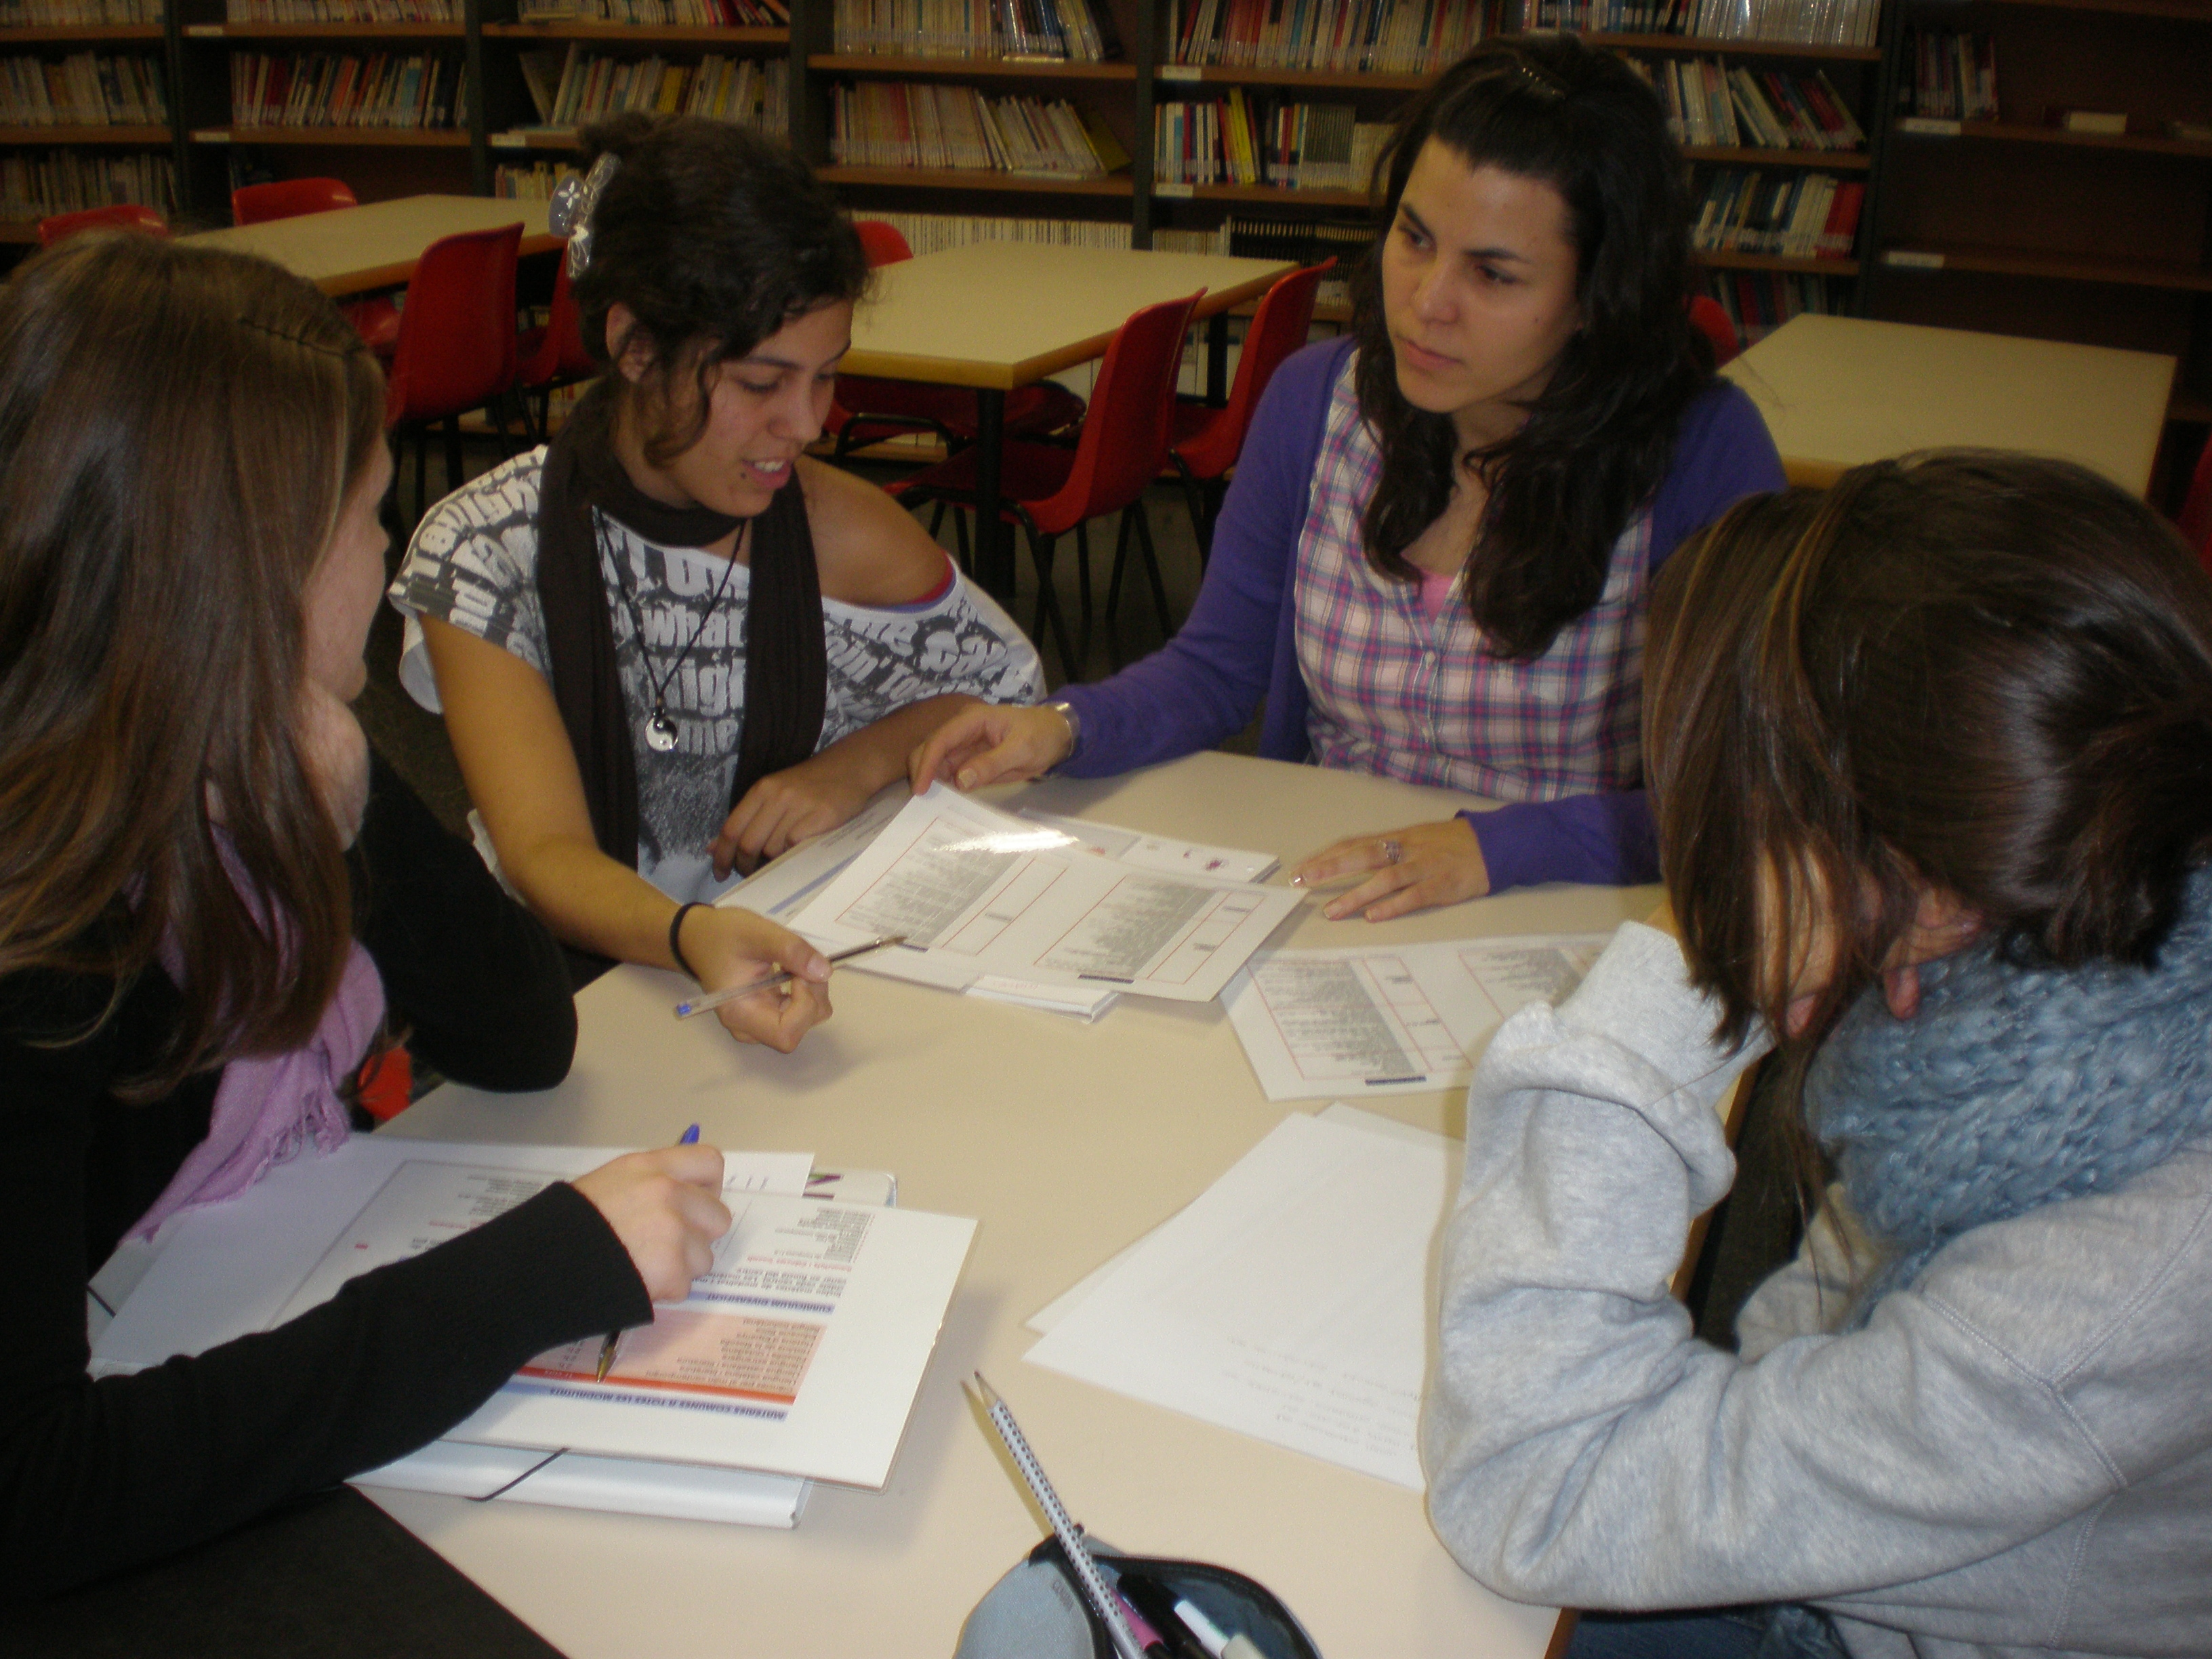
\includegraphics[width=9cm,keepaspectratio]{eso/img/Aulamobil3.JPG}

El passat mes 21 d’octubre es va instal·lar a la nostra escola l’aula mòbil per a les professions destinada a l’alumnat de 4t d’ESO.

Els nois i noies hi van trobar un enorme cabdal d’informació sobre els estudis que tenen al seu abast quan acabin l’ESO i les professions existents que s’hi relacionen.

Es van tractar temes com ara:

\begin{itemize}

	\item La formació professional. Els cicles formatius de grau mitjà: totes les especialitats, requisits d’accés, sortides professionals dels estudis, els centres de formació on s’imparteixen i l’accés posterior als de grau superior.

	\item El Batxillerat: les diferents modalitats i la correspondència amb la Universitat i amb la formació professional de grau superior.

	\item La Universitat. Les proves d’accés, les notes de tall, les noves carreres universitàries de l’espai europeu, les universitats i els centres adscrits, les passarel·les entre carreres, els plans d’estudi, etc.

	\item Els ensenyaments artístics i especialitzats. Els cicles formatius de grau mitjà d’arts plàstiques i disseny, el teatre, la dansa i la música

	\item Les sortides professionals corresponents a cada estudi i els perfils recomanats en cada ensenyament. 

\end{itemize}

\end{news}


\begin{news}
{2} %columnes
{Sortida al CaixaForum}
{Miquel Barceló – La Solitude Organisative}
{ESO}
{12} %pagesof


\noindent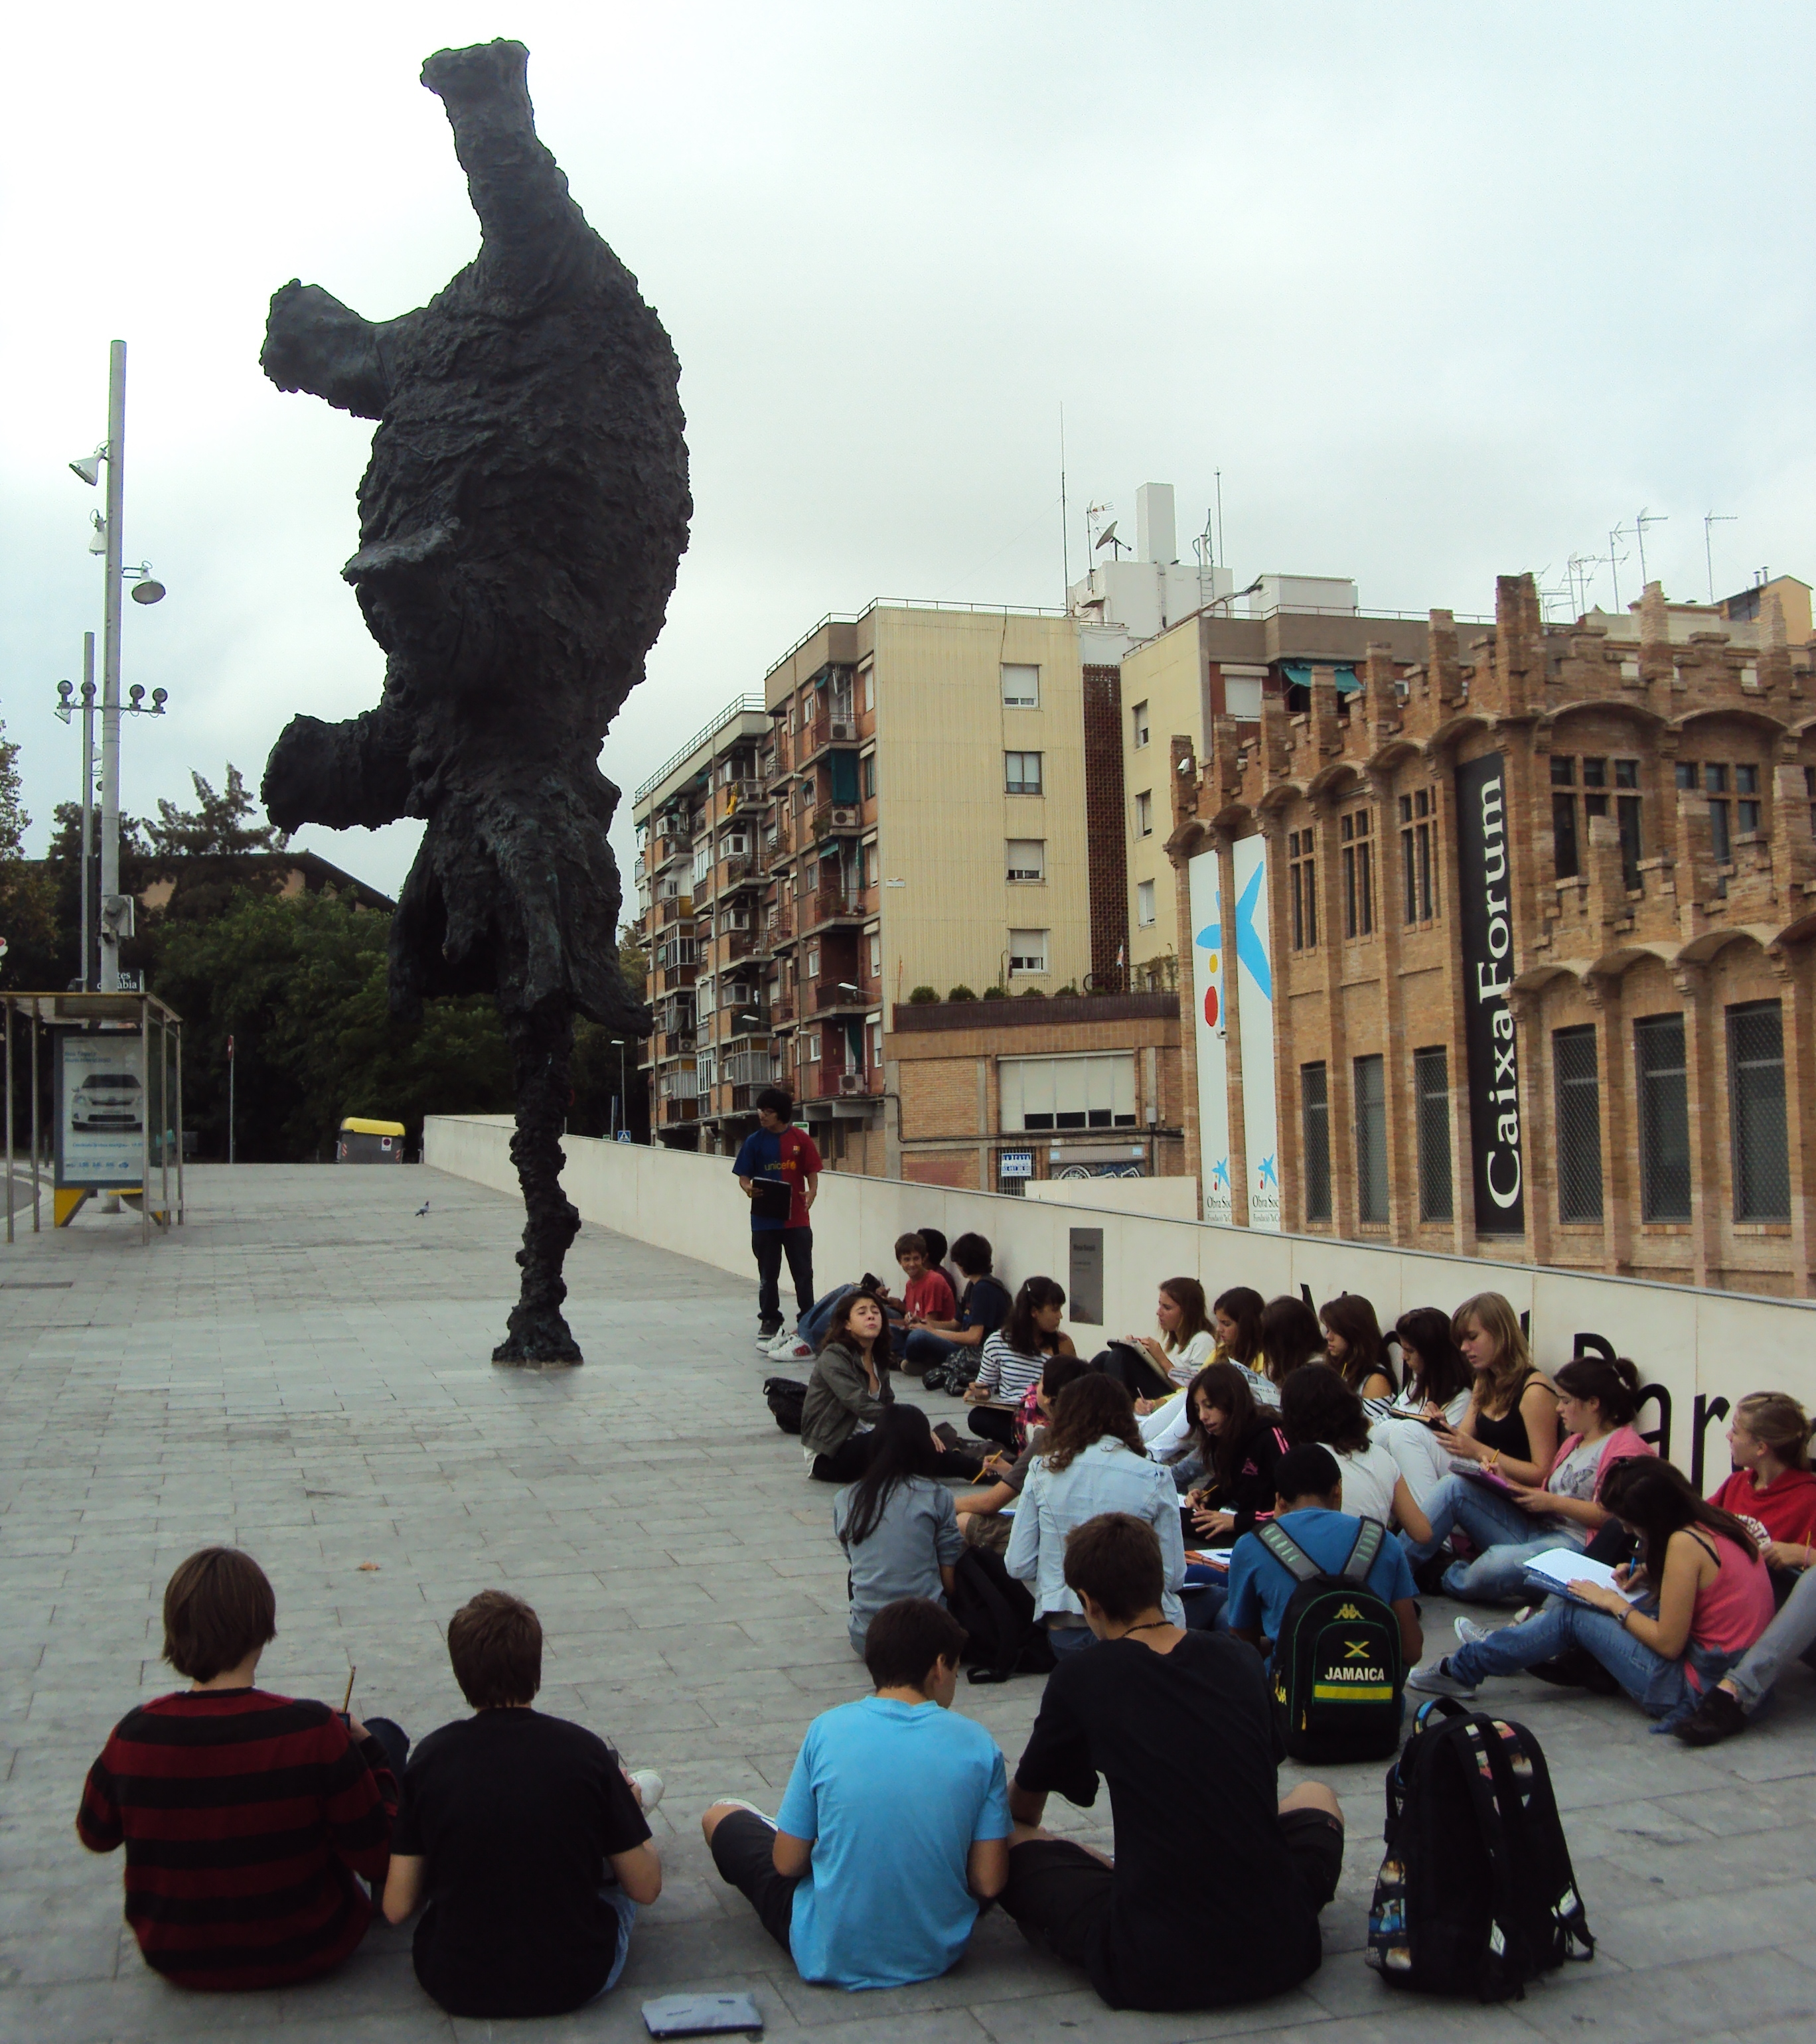
\includegraphics[width=7cm,keepaspectratio]{eso/img/barcelo_2.jpg}

Miquel Barceló.
Miquel Barceló és un pintor mallorquí caracteritzat, entre altres coses, per pintar quadres amb volum, com per exemple el quadre d'una paella, on hi enganxa arròs real. Va estudiar a París, Mali i Mallorca. No creu en Déu, ho demostra amb un quadre en el que canvia la imatge de Jesús crucificat, per un conill crucificat. L’artista també es caracteritza per fer escultures de bronze.

Exposició.
En el primer quadre hi surt ell envoltat de llibres i paisatges en procés d'excitació, cosa que ens vol donar a entendre que li encanten els llibres, els quadres, els paisatges naturals, i que té un gran potencial artístic.

La segona obra és un quadre on hi apareixen diferents animals entre els quals destaca una cabra. En aquesta obra es pot veure una característica de Barceló: dóna volum als seus quadres a l’atzar i, depenent de la forma que adoptin, hi pinta a sobre, improvisant.

Al tercer quadre hi apareix una paella amb arròs real enganxat. També hi apareixen altres aliments com musclos, tomàquets i altres tipus de marisc i d’hortalisses. 

Al quart quadre hi apareixen dues papaies. Aquesta obra es caracteritza perquè la va pintar davant de casa seva, al carrer. El paper del quadre està arrugat perquè la pintura s’escampi per les petites arrugues de la làmina.

L’ obra següent representa un retrat d’un amic seu de l’Àfrica. Es caracteritza perquè ha aprofitat el paper de les papaies per pintar-hi darrere.
 
La sisena obra és una vitrina amb diferents escultures petites fetes amb fang i de diferents formes.

El setè quadre representa la sorra del desert d’Àfrica, pintada d’un blanc trencat, ja que en aquell moment la llum del Sol l’enlluernava.

La vuitena obra és un “collage” de gossos, ja que els compara amb els humans.

A la novena obra hi apareixen diferents quadres de pobles pobres, indígenes, en una paret. Aquest quadre es caracteritza perquè Barceló va deixar el quadre sense pintar al seu estudi i,  quan va tornar, els tèrmits havien fet forats al quadre i ell, en comptes de llençar-lo, va trobar-lo encara més interessant i hi va pintar a sobre, aprofitant els forats.

La desena obra són quadres fets amb elements de la naturalesa (pintures sintètiques, sang d'animals, etc...).

L’onzena obra són diferents quadres en blanc, negre i marró en una sala fosca. Els va pintar a la nit. Amb la foscor vol representar el fons marí, perquè li agradava molt bussejar per les platges de Mallorca.

La darrera obra és una sala de fons vermell amb diferents quadres, uns amb volum i d’altres sense. Hi ha un retrat de la seva biògrafa; també un retrat del seu marxant, i un autoretrat seu. És l’ obra més gran i més destacada de l’ exposició, en la qual es representa a ell mateix com un goril·la, per la seva solitud: d’aquí ve el títol de l’exposició La Solitude Organisative.

\authorandplace{Eduard Ferrusola i Davínia Vilagrasa}{ESO}
\end{news}


%doc: Aprendre democracia/APRENDRE DEMOCRACIA.doc
\begin{news}
{2} %columnes
{Aprendre Democràcia}
{El grup de 4t d’ESO ha estat treballant, durant tot aquest primer trimestre, en els continguts del programa “Aprenem a votar”}
{ESO}
{518} %pagesof

%\noindent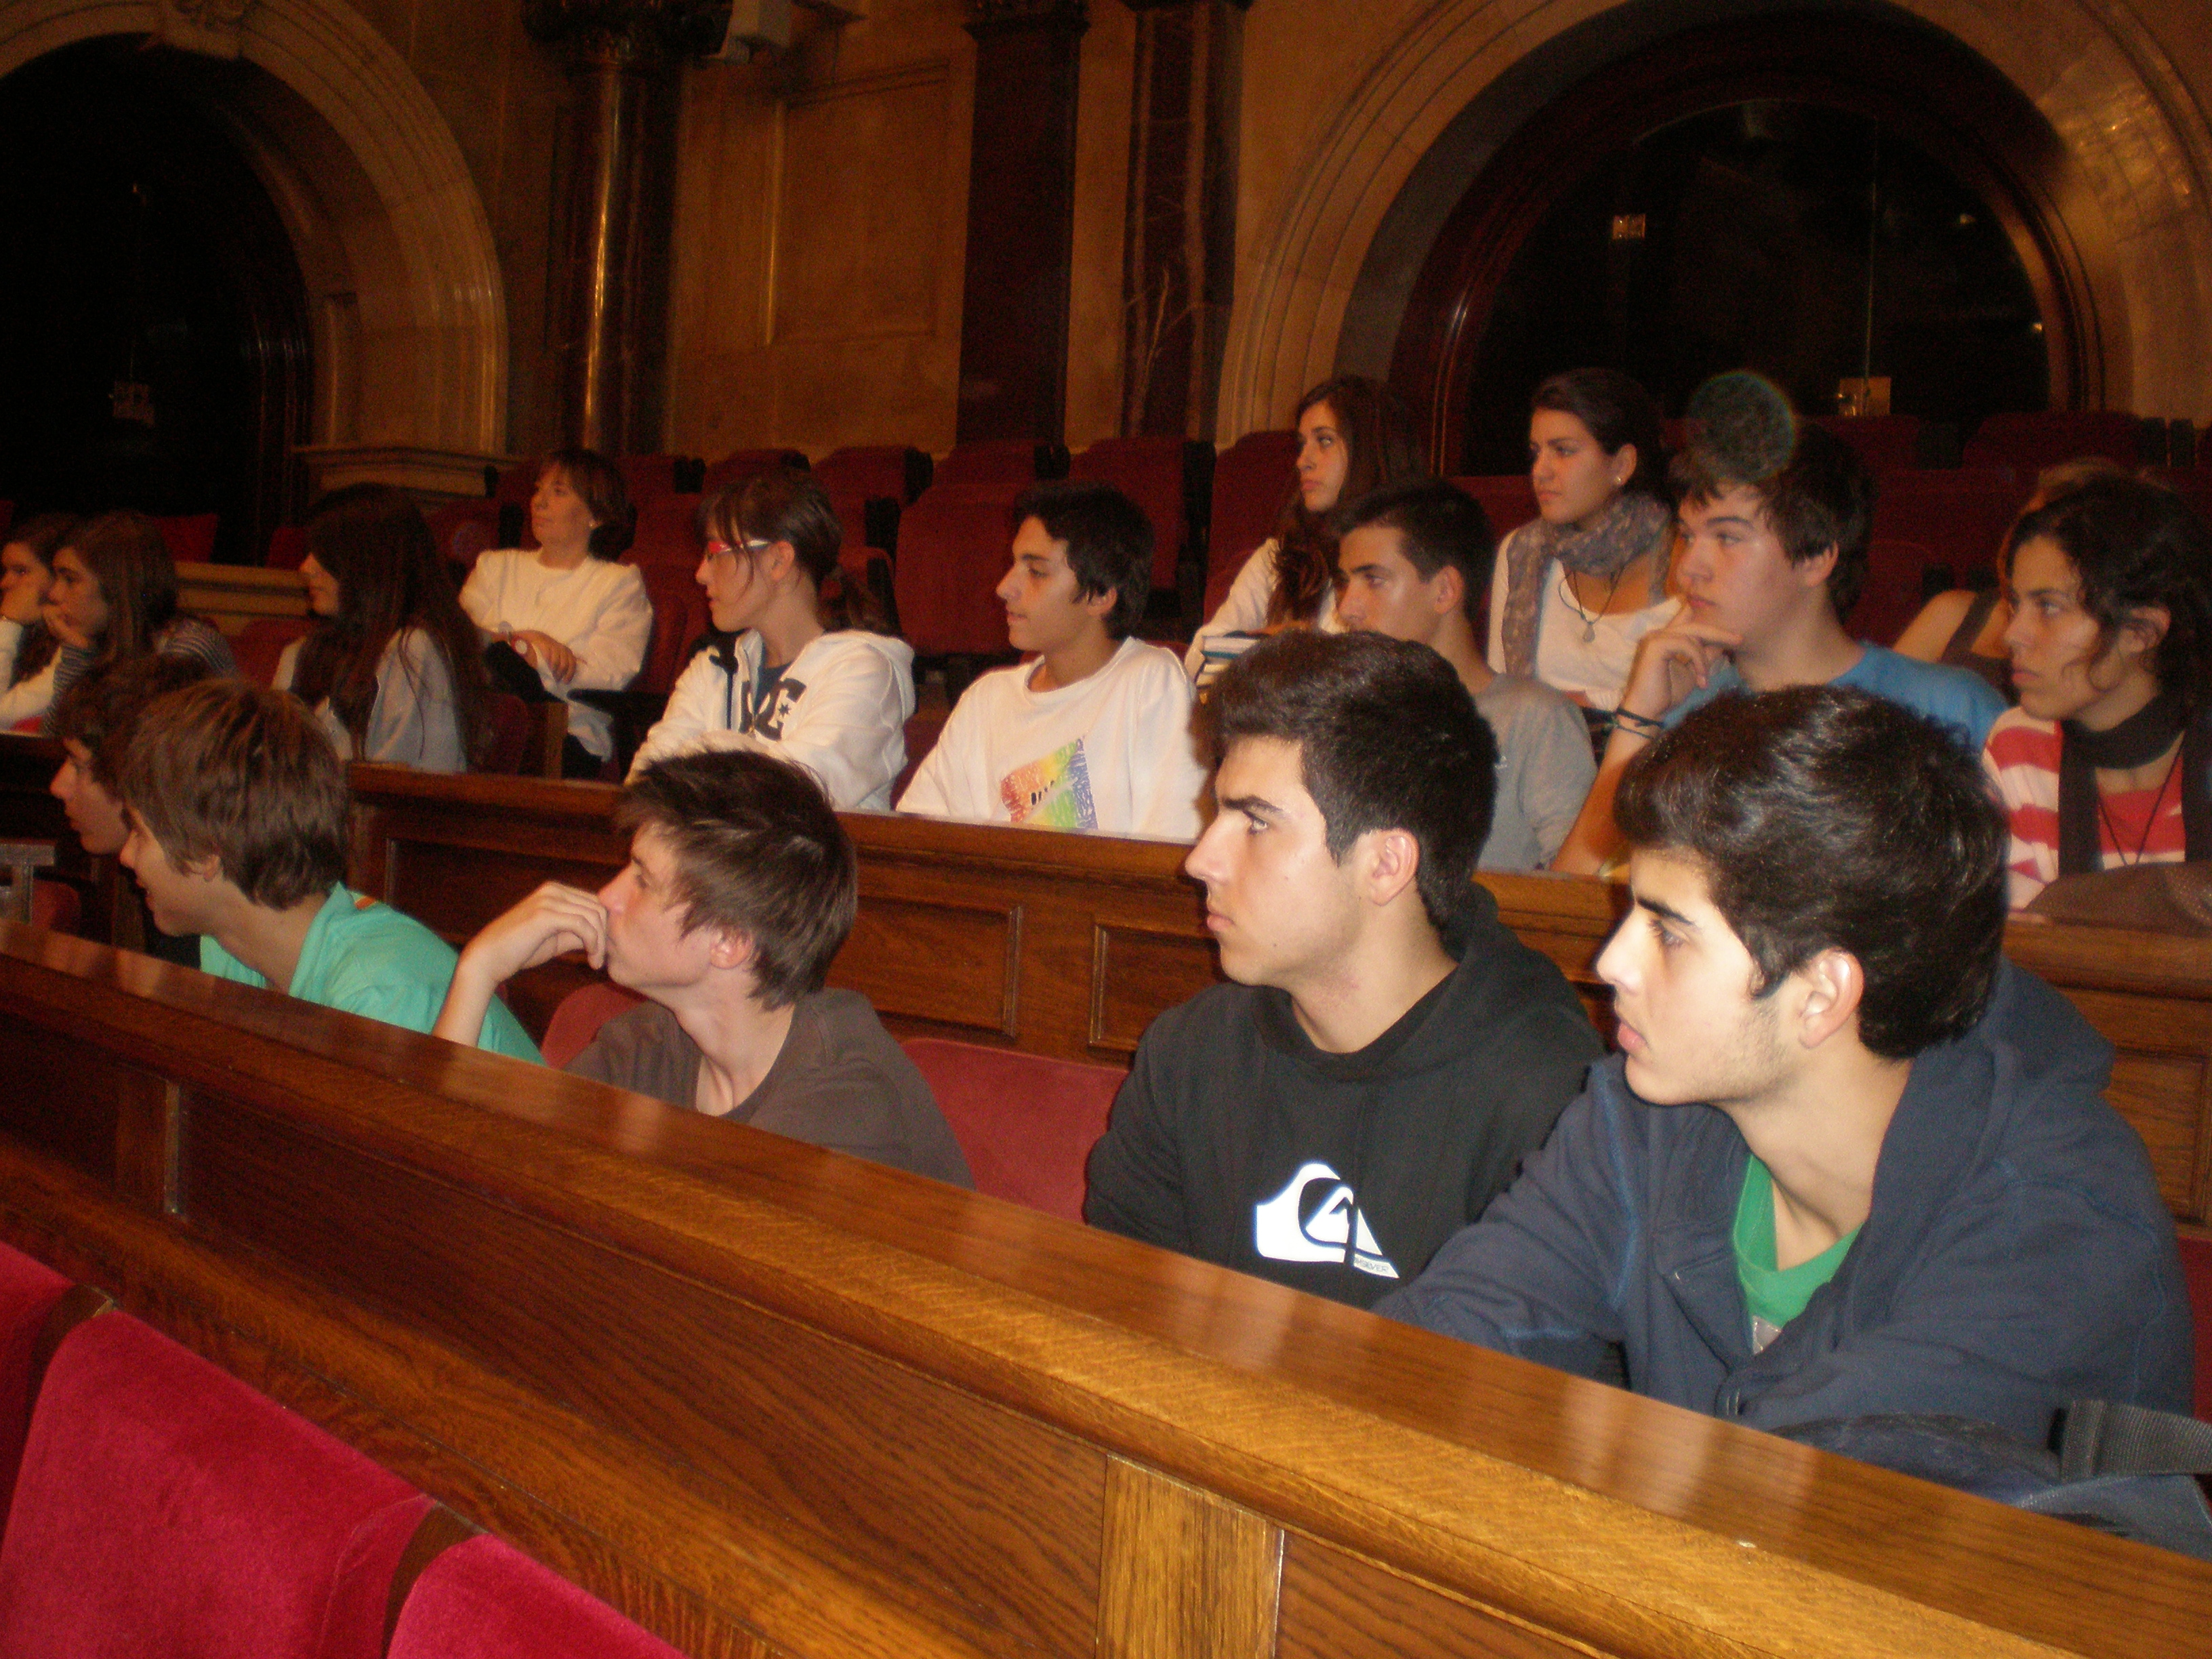
\includegraphics[width=7cm,keepaspectratio]{eso/img/PA220021.JPG}

El nois i noies han anat aprenent que el vot  és una de les diferents maneres d’implicació i de participació política en una democràcia i, tot i que encara no tinguin la majoria d’edat,  van ser convidats a fer una simulació que, de segur, tindrà un impacte important tant en els seus coneixements com en els coneixements que la societat té del que pensa i vol la gent jove.

El nostre centre escolar i el nostre grup de 4t d’ESO han estat escollits per dur a terme aquest procés d’aprenentatge. A través dels exercicis han pogut  conèixer en detall com funcionen les eleccions a Catalunya i com està establert el circuit de representació ciutadana. Els nois i noies, sens dubte,  han fet un exercici de participació molt important per a la vida del nostre país. 

En les fotografies podem veure diferents moments de la visita del grup de 4t de Secundària al Parlament, visita que s’inscrivia dins aquest programa “Aprenem a votar”.

\end{news}

%\noindent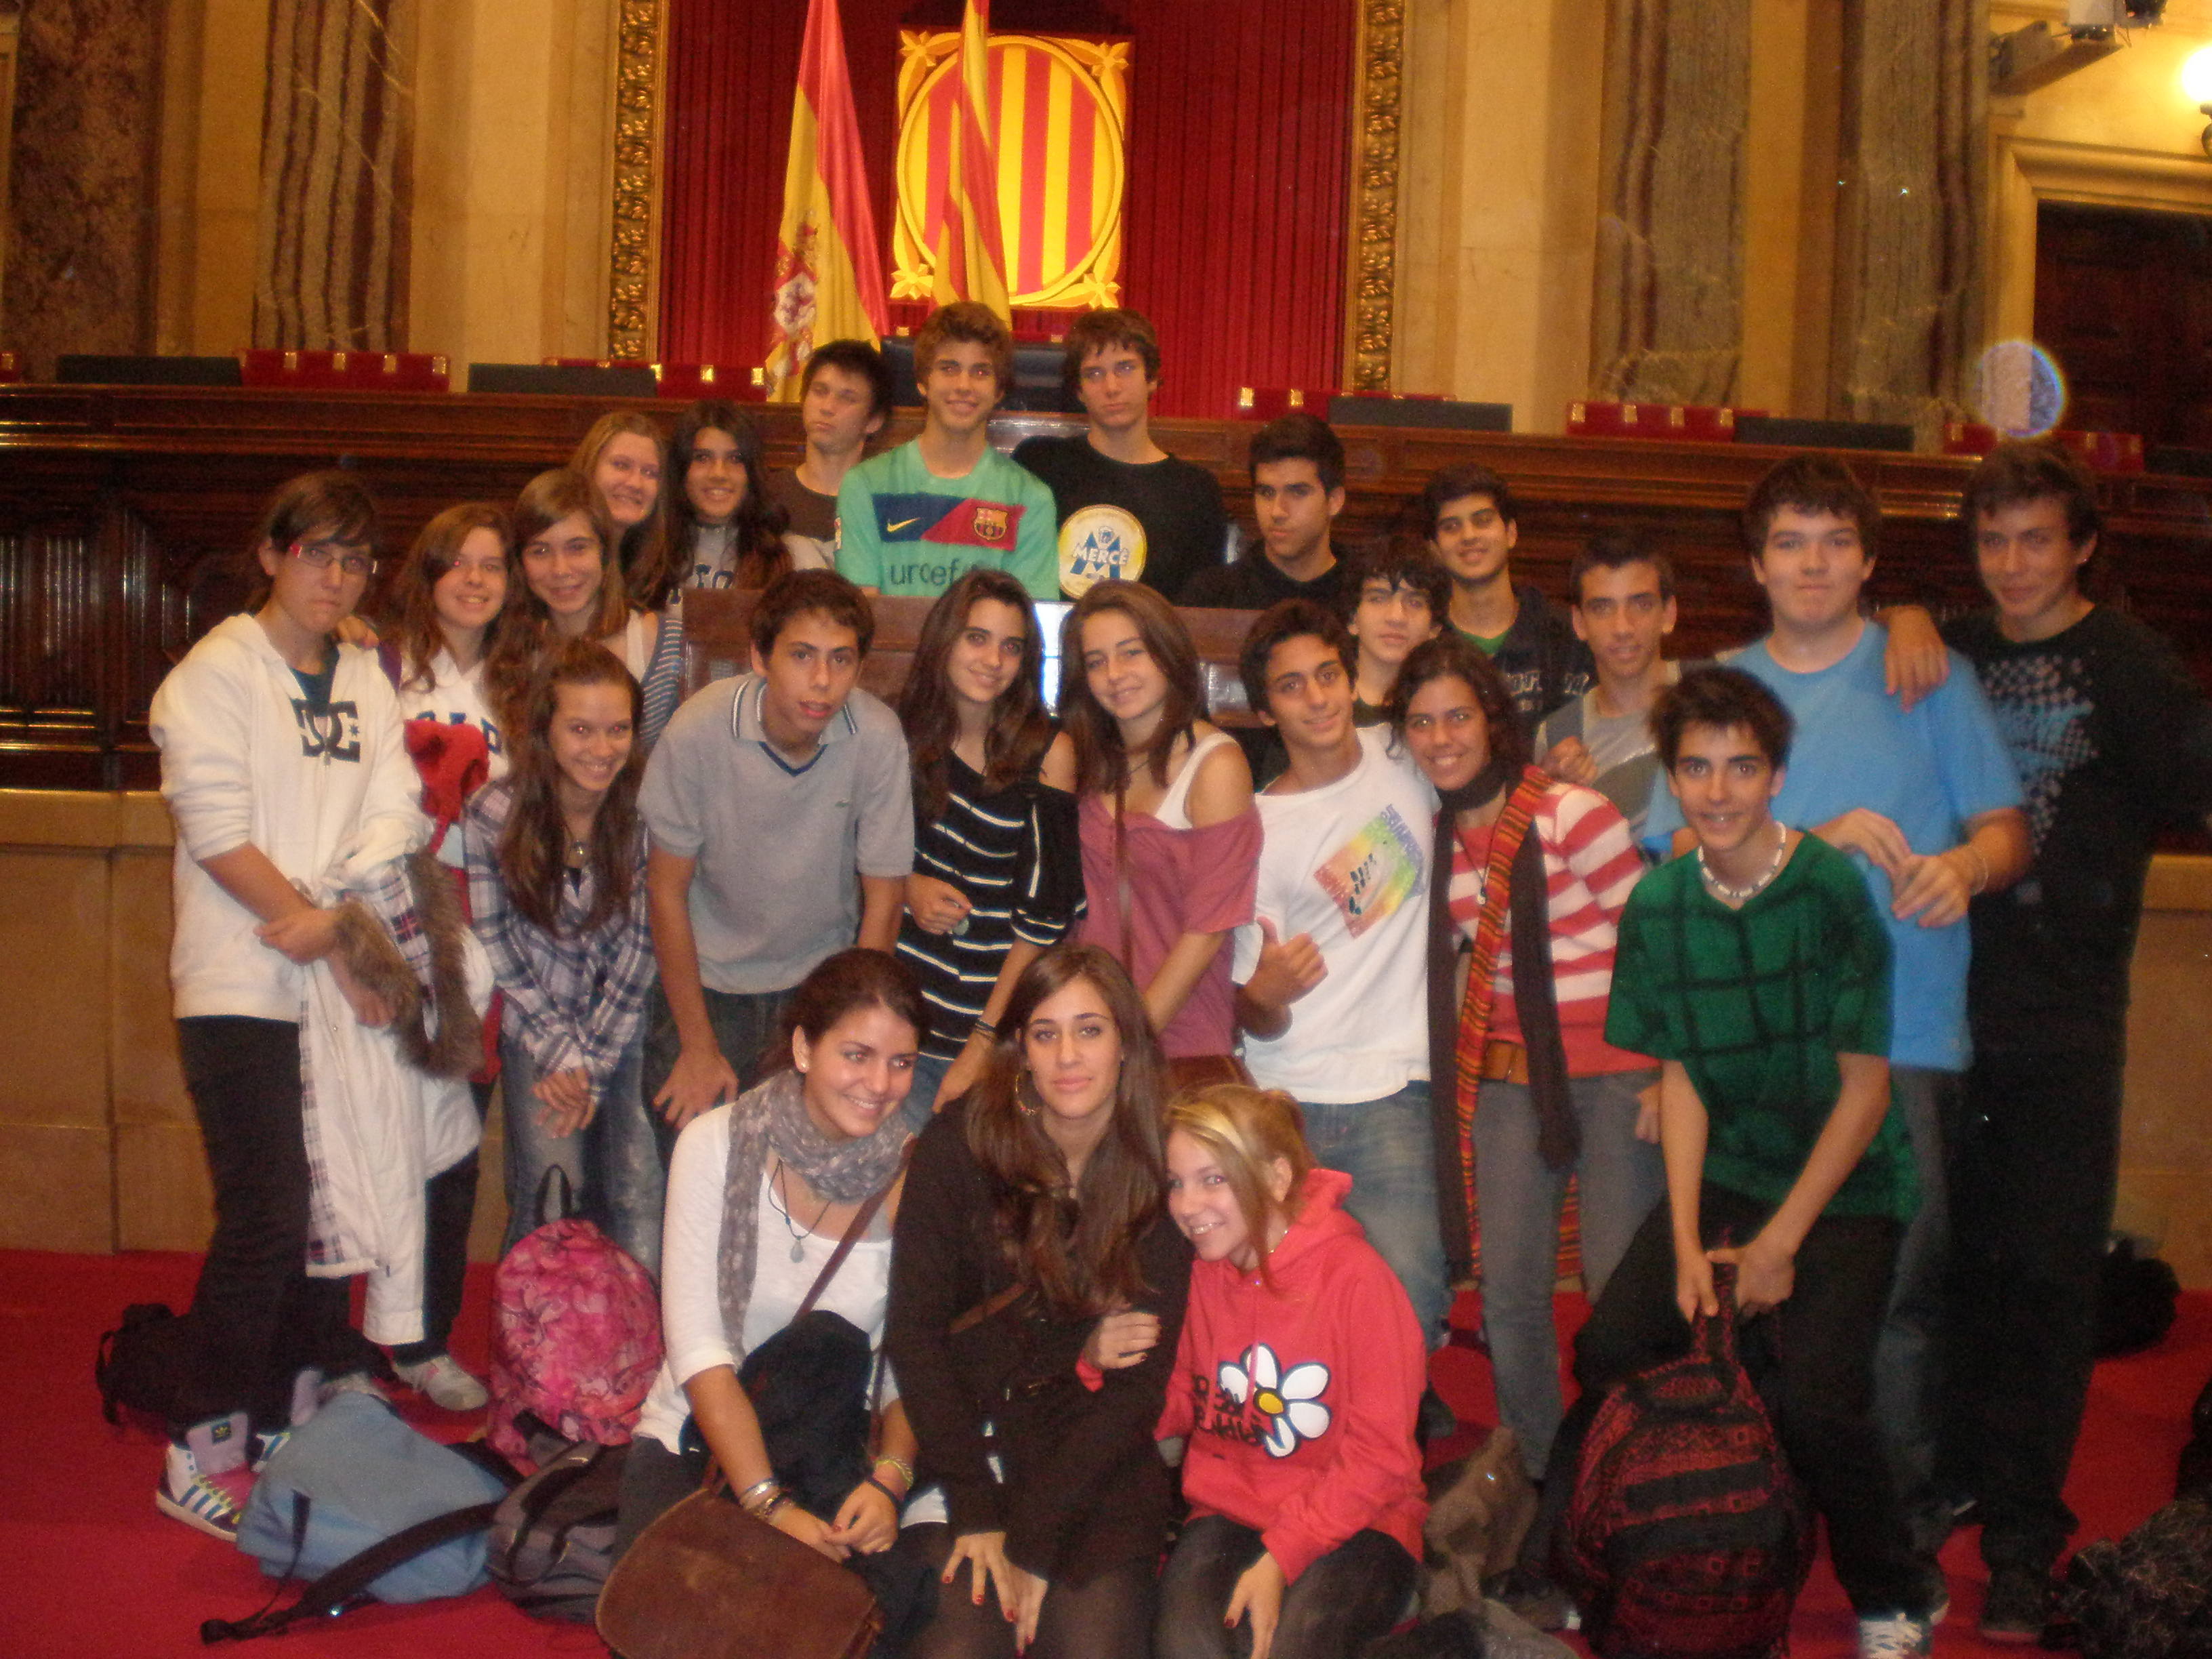
\includegraphics[width=18cm,keepaspectratio]{eso/img/PA220024.JPG}



\begin{news}
{2} %columnes
{Sortida Pipilotti Rist}
{\noindent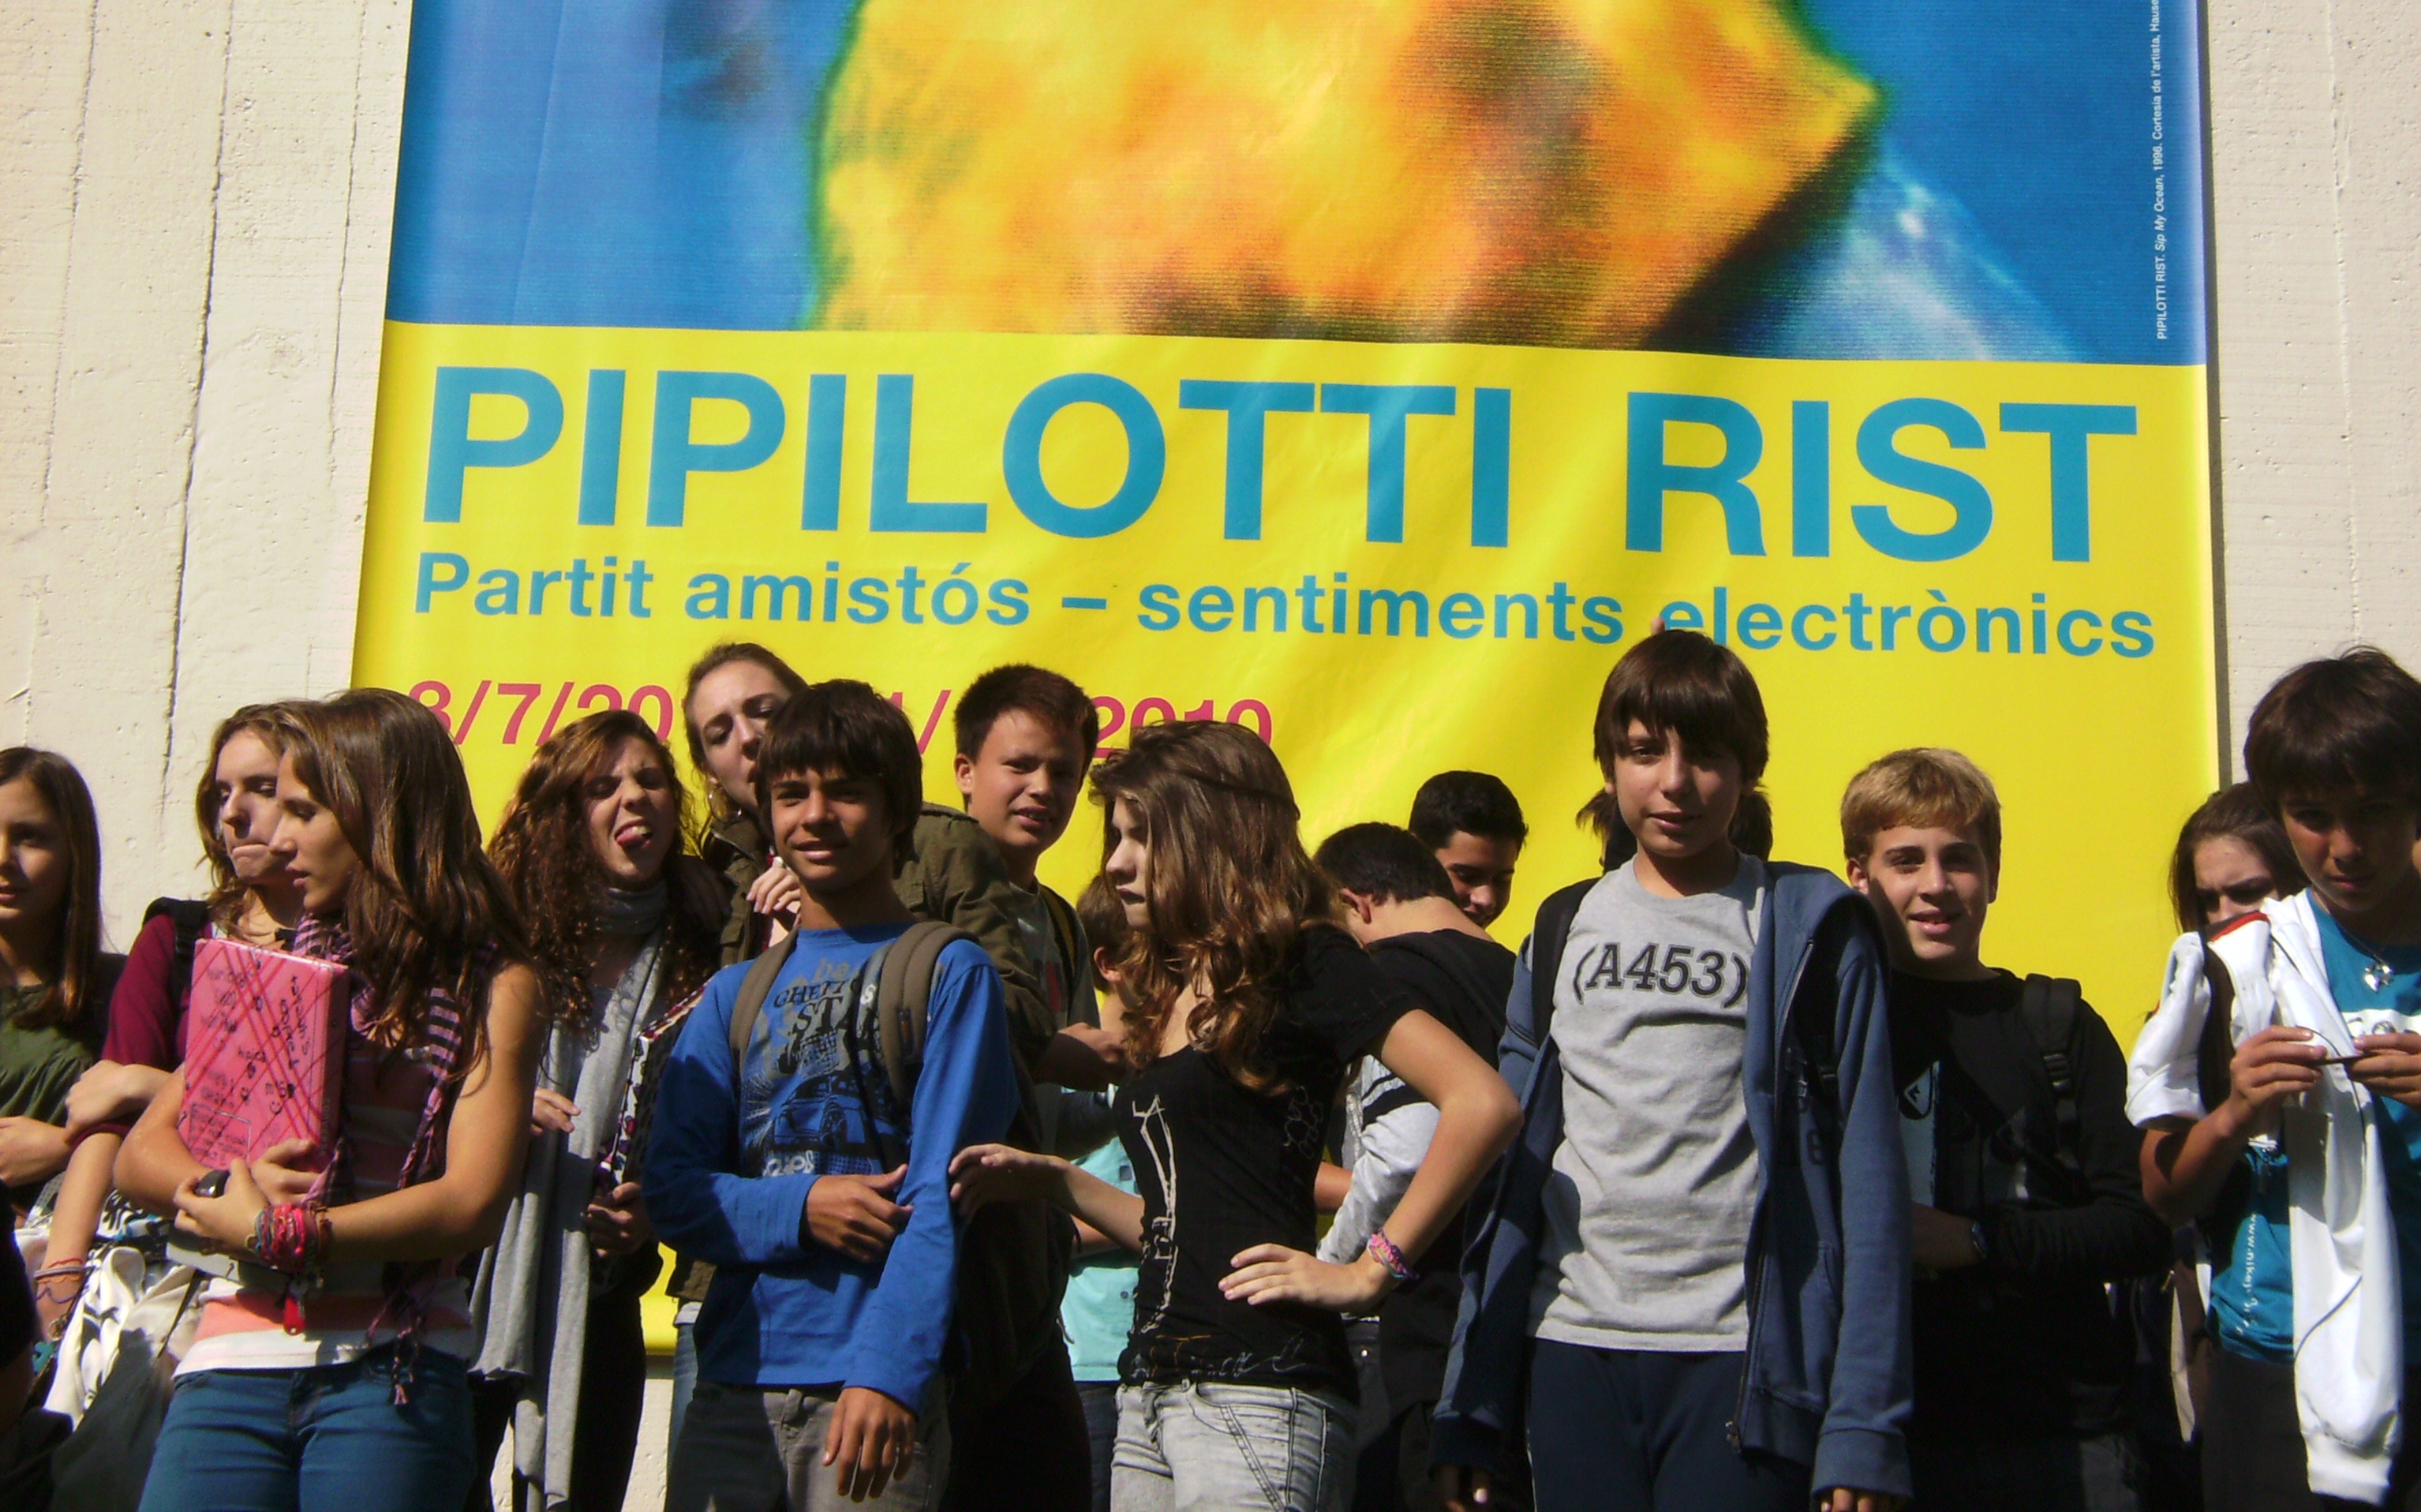
\includegraphics[width=16cm,keepaspectratio]{eso/img/pipilotib.JPG}}
{ESO}
{13} %pagesof

El divendres 22 d'octubre els alumnes de 2n d'ESO vam anar a la Fundació Miró a veure una exposició de la Pipilotti Rist.


%doc: 2a tramesa revista/SORTIDA PIPPILOTI RIST/Pipilotti Rist- Ccalvo i Mromero.doc

La Pipilotti Rist és una artista que treballa sobretot amb vídeo, d’aquesta manera ella vol intentar que entris en les seves obres art, cosa que no es pot fer amb els quadres. 


Vam entrar  a quatre sales. En la primera sala, que es diu “ Xarrupa el meu oceà” parla del desig profund d’entendre’ns els uns amb els altres. En aquesta sala l’artista juga amb dues pantalles fent cantonada i  les imatges que surten alhora, surten simètriques l’una i altra.  Aquest vídeo és una queixa personal per part de l’artista, que diu que està sola  ja que, a l’ haver-hi dues pantalles, ens vol dir que aquell univers està format per dues persones, però només hi és  ella.

La segona sala consta de dues obres. Una obra està formada  per una làpida, unes fulles i un  vídeo d’ella mateixa, d’aquesta manera ens vol fer veure que solament el nom de la persona a la làpida no diu res, que seria millor que hi hagués un vídeo de la vida de la persona morta. La segona obra està formada per un vídeo de dos nens petits jugant en una piscina buida, d’aquesta manera vol relacionar la fragilitat de l’estructura òssia dels nens petits amb la fragilitat del món actual, tant en la política com en l’economia...

La tercera sala està formada per una sala blanca amb una cuina amb armaris que arriben fins al sostre, fent de pantalla per la projecció d’un vídeo en el qual surt ella sota la pluja, i  la pluja representa el seu plor en sentir-se sola a la cuina treballant pels altres.

I la quarta sala està formada per tres pantalles, dues paral·leles perpendiculars a una altra de frontal. Aquesta obra s’anomena “L’òvul pulmonar” I tracta de la nostra autocensura diària. Això l’artista ho aconsegueix amb la seva imitació cap a la natura. És a dir,  en una pantalla es veu un porc senglar i a l’altra se la veu a ella imitant-lo.


Generalment les seves obres parlen d’ella mateixa i de la seva posició com a dona.

\authorandplace{Clàudia Calvo i Marina Romero}
{3r d’ESO}



%doc: 2a tramesa revista/SORTIDA PIPPILOTI RIST/pipilotti.doc

Quan vam arribar, vàrem deixar les motxilles en unes  taquilles i vam començar la visita.

Vam veure diferents vídeos. Primer vam entrar en una sala i ens vam estirar a terra. L'autora explicava els seus sentiments d'amor; es veia el fons del mar i se sentia una cançó d'amor  que cantava ella.

Després vam anar a una altra sala, en aquesta ens havíem d'estirar sobre uns coixins  perquè el vídeo es projectava al sostre.

Hi havia una altra obra que era una escultura, a dins d'una de les peces hi havia el projector. Representava un mòbil, en el qual hi havia una bola de metall a un costat i , a l'altre,  una peça de roba que era una gota.

Seguidament, vam veure un vídeo que estava projectat per tres càmeres on es veien imatges diferents, però que estaven relacionades entre elles.

Per acabar hi havia una sala que representava una cuina on es veia projectat un vídeo que explicava els sentiments d'una dona maltractada.

En acabar la visita, vàrem anar a dinar a fora. Després vam tornar a l'escola.

Aquesta sortida ens va agradar molt a tots, ja que era un tipus d'art més actual, que nosaltres tenim més present.

\authorandplace{Marta Ortega
Marina Jiménez}{ESO}


\end{news}






\end{document}
